%\documentclass[a4paper,12pt]{book}
\documentclass[oneside, a4paper]{book}
%\usepackage{amsmath,amsxtra,amssymb,latexsym, amscd,amsthm, array}
\oddsidemargin0mm
\textwidth154mm
\parskip2mm
\parindent0mm
\usepackage{array}
\usepackage{multirow}
\usepackage{tabularx}
\usepackage{microtype}
\usepackage{cite}
\usepackage{indentfirst}
\usepackage{enumitem}
\usepackage{float}
\usepackage{graphicx}
\usepackage{wrapfig}
\usepackage{tikz, pgf} 
\usetikzlibrary{patterns}
\usepackage{float}
\usepackage{listings}
\usepackage{xcolor}
\definecolor{codegreen}{rgb}{0,0.6,0}
\definecolor{codegray}{rgb}{0.5,0.5,0.5}
\definecolor{codepurple}{rgb}{0.58,0,0.82}
\definecolor{backcolour}{rgb}{0.95,0.95,0.92}
\lstdefinestyle{mystyle}{
	backgroundcolor=\color{backcolour},   
	commentstyle=\color{codegreen},
	keywordstyle=\color{magenta},
	numberstyle=\tiny\color{codegray},
	stringstyle=\color{codepurple},
	basicstyle=\ttfamily\footnotesize,
	breakatwhitespace=false,         
	breaklines=true,                 
	captionpos=b,                    
	keepspaces=true,                 
	numbers=left,                    
	numbersep=5pt,                  
	showspaces=false,                
	showstringspaces=false,
	showtabs=false,                  
	tabsize=2
}
\lstset{style=mystyle}
\usepackage{amsmath,amssymb,latexsym,amscd,amsxtra,graphicx,graphpap,amsthm}
\usepackage{mathtools}
\usepackage{pb-diagram}
\usepackage{indentfirst}
\usepackage{caption}
\usepackage{aligned-overset}
\usepackage{picinpar,floatflt}
\usepackage{longtable}
\usepackage{fancybox}
\usepackage[utf8]{vietnam}
\usepackage[utf8]{inputenc}
\usepackage[tight,vietnam]{minitoc}
\usepackage{anyfontsize}
% hyperref chỉ được nạp một lần và nên nạp gần cuối phần package
\usepackage[hidelinks]{hyperref}
\Urlmuskip=0mu plus 1mu
%\usepackage{commath}
%==================================
\usepackage{titletoc}
\titlecontents{chapter}
[0pt]
{\bfseries}
{\chaptername\ \thecontentslabel\enskip}
{}
{\hfill\contentspage}
%==================================

%==================================
\renewcommand{\thechapter}{\arabic{chapter}}
\renewcommand{\thesection}{\arabic{chapter}.\arabic{section}}
\newcommand{\eproof}{\hfill $\square$}
%\newcommand{\eproof}{\hfill}
\newcommand{\chm}{{\bfseries Chứng minh.}}
\newenvironment{cm}{\chm}{\eproof}
%===============================
\theoremstyle{plain}

\theoremstyle{plain}
\newtheorem*{theorem}{Định lý}
\newtheorem*{definition}{Định nghĩa}
\newtheorem{proposition}{Mệnh đề}
\newtheorem*{remark}{Nhận xét}
\theoremstyle{remark}
\newcommand{\wcon}{\rightharpoonup}
\newtheorem{example}{Ví dụ}
\newtheorem{lemma}{Bổ đề}

\theoremstyle{definition}
\newtheorem{dn}{Định nghĩa}[chapter]
\providecommand*{\dnautorefname}{Định nghĩa}
\newtheorem{bt}[dn]{Bài toán}
\providecommand*{\btautorefname}{Bài toán}
\newtheorem{vd}[dn]{\bfseries Ví dụ}
\providecommand*{\mdautorefname}{Mệnh đề}

\newtheorem{bd}[dn]{Bổ đề}
\providecommand*{\bdautorefname}{Bổ đề}
\newtheorem{md}[dn]{Mệnh đề}
\providecommand*{\mdautorefname}{Mệnh đề}
\newtheorem{hq}[dn]{Hệ quả}
\providecommand*{\hqautorefname}{Hệ quả}
\newtheorem{dl}[dn]{\bfseries Định lý}
\providecommand*{\dlautorefname}{Định lý}
\newtheorem{algorithm}{\bfseries Thuật toán}[chapter]
\providecommand*{\algorithmautorefname}{Thuật toán}
\newtheorem*{namedthm}{\namedthmname}
\newcounter{namedthm}
\makeatletter
\newenvironment{named}[1]
{\def\namedthmname{#1}%
	\refstepcounter{namedthm}%
	\namedthm\def\@currentlabel{#1}}
{\endnamedthm}
\makeatother

\theoremstyle{remark}
\newtheorem{kh}[dn]{ký hiệu}
\newtheorem{nx}[dn]{\bf Nhận xét}
\newtheorem{cy}[dn]{Chú ý}
\renewenvironment{proof}{{\bfseries \itshape Chứng minh }}

\renewcommand{\baselinestretch}{1.5}
\setlength{\oddsidemargin}{0.3cm}     %Lề trái tính từ điểm cách mép giấy 2.54cm
\setlength{\topmargin}{-1cm}          %Lề trên tính từ điểm cách mép giấy 2.54cm
\setlength{\headsep}{0.5cm}                %Khoang cach tu  Headerline tới Khối chữ
\textwidth=15.5cm
\textheight=24.5cm
\renewcommand{\bibname}{Tài liệu tham khảo}
\renewcommand{\large}{\fontsize{14pt}{14pt}\selectfont}
\renewcommand{\Large}{\fontsize{16pt}{16pt}\selectfont}
\renewcommand{\LARGE}{\fontsize{15pt}{15pt}\selectfont}
\renewcommand{\th}{\fontsize{18pt}{18pt}\selectfont}
\makeatletter

\makeatother


\newenvironment{mproof}{\paragraph{Chứng minh:}}{\hfill$\square$}
\newenvironment{myproof}[2] {\paragraph{Proof of {#1} {#2} :}}{\hfill$\square$}
\DeclarePairedDelimiter{\pro}{\langle}{\rangle}
\DeclarePairedDelimiter{\norm}{\lVert}{\rVert}
\DeclarePairedDelimiter{\abs}{\lvert}{\rvert}
\usepackage{xpatch}
\makeatletter
\AtBeginDocument{\xpatchcmd{\@thm}{\thm@headpunct{.}}{\thm@headpunct{}}{}{}}
\makeatother

\usepackage{fancyhdr}
\usepackage{xcolor} % cho số trang màu

\pagestyle{fancy}
\fancyhf{}

% Footer trái: tên sinh viên
\fancyfoot[L]{\textcolor{black}{Nguyễn Hữu Nhật Anh - 20237412}}

% Footer phải: số trang màu đỏ
\fancyfoot[R]{\textcolor{red}{\thepage}}

% Gạch ngang trên footer
\renewcommand{\footrulewidth}{0.4pt}
\renewcommand{\headrulewidth}{0pt}

\fancypagestyle{plain}{
	\fancyhf{}
	\fancyfoot[L]{\textcolor{black}{Nguyễn Hữu Nhật Anh - 20237412}}
	\fancyfoot[R]{\textcolor{black}{\thepage}}
	\renewcommand{\footrulewidth}{0.4pt}
	\renewcommand{\headrulewidth}{0pt}
}


\begin{document}
	
	
	\thispagestyle{empty}
	%\thispagestyle{headings}
	\setcounter{page}{1}%
	\pagenumbering{arabic}
	%\addcontentsline{toc}{chapter}{{Trang bìa phụ}}
	%\newgeometry{top=2.0cm,bottom=3.0cm,left=3.5cm,right=2.8cm}
	%\begin{titlepage}
	
	%\setlength{\fboxrule}{1pt}
	%\thisfancypage{\setlength{\fboxsep}{2pt}\setlength{\fboxrule}{2pt}\doublebox}{} 
	%\setlength{\fboxrule}{1pt}
	%\thisfancypage{\setlength{\fboxsep}{0pt}\setlength{\shadowsize}{0pt}\doublebox}{}
	\pagenumbering{arabic}
	%\newgeometry{left=2.8cm,right=1.8cm,top=2.5cm,bottom=2cm}
	\begin{tikzpicture}[remember picture,overlay,inner sep=0,outer sep=0]
		\draw[blue!70!black,line width=2.5pt] ([xshift=-1cm,yshift=-2cm]current page.north east) coordinate (A)--([xshift=2cm,yshift=-2cm]current page.north west) coordinate(B)--([xshift=2cm,yshift=2cm]current page.south west) coordinate (C)--([xshift=-1cm,yshift=2cm]current page.south east) coordinate(D)--cycle;
	\end{tikzpicture}
	\begin{center}
		\Large
		\vspace{-1cm}
		{\bfseries ĐẠI HỌC BÁCH KHOA HÀ NỘI}\\
		{\bfseries KHOA TOÁN-TIN}
		
	\end{center}
	\vspace{1cm}
	\begin{center}
		\fontsize{17pt}{15pt}\selectfont
		
\includegraphics[scale=0.5]{hust.jpg}
		\vspace{1cm}
		
		\fontsize{22pt}{15pt}\selectfont
		\bfseries PHÂN TÍCH DOANH SỐ VÀ XU HƯỚNG TIÊU DÙNG KHÁCH HÀNG TRONG LĨNH VỰC BÁN LẺ
		
		
	\end{center}
	
	\vspace{0.8cm}
	\begin{center}
		\fontsize{16pt}{16pt}\selectfont 	
		{\bfseries ĐỒ ÁN I}\\	
		\fontsize{14pt}{16pt}\selectfont
		{\bfseries Chuyên ngành: Hệ thống Thông tin Quản lý}\\
	\end{center}
	
	\vspace{1cm}
	\begin{center}
		\fontsize{13pt}{16pt}\selectfont
		\textbf{\begin{tabular}{l l}
				Giảng viên hướng dẫn:& TS. Đoàn Duy Trung\\
				Sinh viên thực hiện:& Nguyễn Hữu Nhật Anh\\
				Mã số sinh viên:& 20237412\\
		\end{tabular}}
		
	\end{center}
	\vspace{1cm}
	\begin{center}
		\LARGE HÀ NỘI -- 2026
	\end{center}
	
	%\restoregeometry
	\newpage
	
	\newpage
	%\newgeometry{left=2.2cm,right=2.8cm,top=2cm,bottom=2cm}
	\thisfancypage{
		\setlength{\fboxsep}{0.5cm}
		\fbox}{}
	\thispagestyle{empty}
	\fontsize{13pt}{16pt}\selectfont
	\bigbreak
	\begin{center}
		{\bfseries NHẬN XÉT CỦA GIẢNG VIÊN HƯỚNG DẪN}
	\end{center}
	\bigbreak
	
	\fontsize{12pt}{14pt}\selectfont
	\begin{enumerate}
		\item [{\bfseries 1.}]{\bfseries Mục tiêu và nội dung của đồ án}
		\begin{enumerate}
			\item Mục tiêu: Phân tích doanh số và xu hướng tiêu dùng khách hàng trong lĩnh vực bán lẻ dựa trên bộ dữ liệu Superstore Sales; từ đó trực quan hóa dữ liệu, xây dựng mô hình dự báo lợi nhuận và phân cụm khách hàng nhằm hỗ trợ đánh giá hiệu quả kinh doanh.
			\item Nội dung: Đồ án gồm các nội dung chính: cơ sở lý thuyết, tiền xử lý và phân tích dữ liệu, xây dựng dashboard Power BI, xây dựng các mô hình hồi quy và phân cụm, so sánh kết quả mô hình, rút ra nhận xét, hạn chế và hướng phát triển. 
		\end{enumerate}
		\item [{\bfseries 2.}] {\bfseries Kết quả đạt được} 
		\begin{enumerate}
			\item Đã thực hiện tiền xử lý, phân tích khám phá dữ liệu và xây dựng dashboard trực quan phục vụ phân tích doanh thu, lợi nhuận, khu vực, sản phẩm, khách hàng và chiết khấu.
			\item Đã xây dựng và đánh giá các mô hình dự báo lợi nhuận gồm hồi quy tuyến tính đa biến, Random Forest, Gradient Boosting và XGBoost; trong đó XGBoost cho kết quả tốt nhất trên tập kiểm tra.
			\item Đã ứng dụng K-Means để phân cụm khách hàng, đồng thời rút ra một số nhận xét thực tiễn hỗ trợ kiểm soát chiết khấu, đánh giá lợi nhuận và định hướng chăm sóc khách hàng.
		\end{enumerate}
		\item [{\bfseries 3.}]{\bfseries Ý thức làm việc của sinh viên:} Sinh viên có thái độ làm việc nghiêm túc, chủ động tìm hiểu tài liệu, thực hiện đầy đủ các nội dung của đồ án và có tinh thần tiếp thu góp ý để hoàn thiện báo cáo.
	\end{enumerate}
	\hspace{0.5\textwidth}
	\begin{minipage}{0.5\textwidth}
		\noindent\begin{center}
			\textit{Hà Nội, ngày     tháng  năm 2026} \\
			Giảng viên hướng dẫn\\ \vspace{2cm}
			\textbf{TS. Đoàn Duy Trung}
		\end{center}	
	\end{minipage}
	%\restoregeometry
	
	\newpage
	\fontsize{22pt}{16pt}\selectfont
	{\bfseries Lời cảm ơn}
	\fontsize{13pt}{16pt}\selectfont
	\bigskip
	\setlength{\parindent}{2em} % thiết lập độ thụt đầu dòng
	\setlength{\parskip}{0.5em} % khoảng cách giữa các đoạn
	
	Trước tiên, em xin gửi lời cảm ơn chân thành tới Thầy – TS. Đoàn Duy Trung – người đã tận tình hướng dẫn và đồng hành cùng em trong suốt quá trình thực hiện đồ án “Phân tích doanh số và xu hướng tiêu dùng khách hàng”. Sự hỗ trợ, những góp ý chuyên môn và định hướng thực tiễn từ Thầy là yếu tố quan trọng giúp em hoàn thành tốt đồ án này.
	
	Trong quá trình làm việc, em học hỏi được rất nhiều từ các lần góp ý của Thầy – từ cách tư duy logic, tổ chức mô hình dữ liệu cho đến việc trình bày rõ ràng, khoa học. Đây là những bài học quý giá giúp em trưởng thành hơn cả về chuyên môn lẫn tác phong làm việc chuyên nghiệp.
	
	Em cũng xin cảm ơn các Thầy, Cô trong Khoa Toán – Tin, Trường Đại học Bách Khoa Hà Nội đã truyền đạt kiến thức và tạo nền tảng vững chắc trong suốt quá trình học tập. Những môn học như Cơ sở dữ liệu, Hệ hỗ trợ quyết định,... đã giúp em triển khai đồ án một cách bài bản và thực tế.
	
	Dù đã nỗ lực hết sức, em hiểu rằng đồ án vẫn còn hạn chế và mong nhận được những góp ý quý báu để tiếp tục hoàn thiện trong tương lai.
	
	Em xin chân thành cảm ơn!
	
	
	
	\bigskip
	
	\begin{minipage}{0.5\textwidth}
	\end{minipage}
	\hspace{0.5\textwidth}
	\begin{minipage}{0.5\textwidth}
		\noindent\begin{center}
			\vspace{1cm}
			\textit{Hà Nội, tháng     năm 2026} \\
			Tác giả đồ án\\ \vspace{2cm}
			\textbf{Nguyễn Hữu Nhật Anh}
		\end{center}	
	\end{minipage}
	
	
	\bigskip
	
	\newpage
	\fontsize{22pt}{16pt}\selectfont
	{\bfseries Tóm tắt nội dung Đồ án}
	\fontsize{13pt}{16pt}\selectfont
	\bigskip
	
	Đồ án tập trung nghiên cứu và phân tích dữ liệu bán hàng dựa trên bộ dữ liệu \textbf{Superstore Sales}, nhằm khai thác các thông tin có giá trị về doanh thu, lợi nhuận, xu hướng tiêu dùng của khách hàng và các yếu tố ảnh hưởng đến hiệu quả kinh doanh. Thông qua quá trình tiền xử lý dữ liệu, phân tích khám phá dữ liệu, trực quan hóa và xây dựng các mô hình phân tích, đồ án hướng tới việc rút ra những nhận xét có cơ sở khoa học, từ đó hỗ trợ đánh giá tình hình kinh doanh một cách khách quan và trực quan hơn.
	
	Nội dung đồ án được triển khai qua bốn phần chính như sau:
	
	\begin{enumerate}
		\item \textbf{Tổng quan lý thuyết:} Trình bày cơ sở lý thuyết liên quan đến phân tích dữ liệu, trực quan hóa dữ liệu và vai trò của dữ liệu trong hỗ trợ ra quyết định. Bên cạnh đó, đồ án cũng giới thiệu các khái niệm nền tảng như thống kê mô tả, phân tích khám phá dữ liệu (Exploratory Data Analysis -- EDA), phân tích mối quan hệ giữa các biến và một số mô hình phân tích dữ liệu thường được ứng dụng trong lĩnh vực kinh doanh.
		
		\item \textbf{Tiền xử lý, phân tích khám phá và trực quan hóa dữ liệu:} Trên cơ sở bộ dữ liệu Superstore Sales, đồ án tiến hành thực hiện các bước tiền xử lý và phân tích khám phá dữ liệu bằng ngôn ngữ \textbf{Python}, sử dụng chủ yếu các thư viện \textbf{pandas} và \textbf{numpy} nhằm kiểm tra cấu trúc dữ liệu, xử lý dữ liệu thiếu, chuẩn hóa kiểu dữ liệu, xây dựng các biến cần thiết và phân tích thống kê ban đầu. Quá trình EDA giúp nhận diện đặc điểm phân bố của dữ liệu, mối quan hệ giữa các biến cũng như những yếu tố nổi bật cần quan tâm trong quá trình phân tích. Sau đó, dữ liệu được trực quan hóa thông qua dashboard xây dựng trên \textbf{Power BI}, tập trung thể hiện các nội dung như xu hướng doanh số theo thời gian, doanh thu và lợi nhuận theo khu vực, nhóm sản phẩm, phân khúc khách hàng, cũng như mối quan hệ giữa chiết khấu, số lượng bán và lợi nhuận. Từ các kết quả trực quan hóa, đồ án tiến hành phân tích và diễn giải các insight nhằm làm rõ những xu hướng và đặc điểm nổi bật của hoạt động kinh doanh.
		
		\item \textbf{Xây dựng mô hình phân tích dữ liệu:} Dựa trên kết quả thu được từ quá trình trực quan hóa và phân tích khám phá dữ liệu, đồ án tiếp tục xây dựng nhiều mô hình phân tích dữ liệu nhằm khai thác sâu hơn bản chất của tập dữ liệu. Các mô hình này được sử dụng để phân tích mối quan hệ giữa các biến, xác định mức độ ảnh hưởng của các yếu tố đến doanh thu và lợi nhuận, đồng thời hỗ trợ phân nhóm, so sánh và nhận diện các đặc điểm tiêu biểu trong dữ liệu. Việc kết hợp nhiều mô hình khác nhau không chỉ giúp nâng cao tính khách quan trong quá trình đánh giá mà còn góp phần củng cố các nhận định đã rút ra từ phần trực quan hóa dữ liệu. Kết quả phân tích mô hình tiếp tục được diễn giải thông qua các insight, làm cơ sở cho việc nhận xét và đánh giá tổng thể.
		
		\item \textbf{Nhận xét, đánh giá và kết luận:} Trên cơ sở tổng hợp kết quả từ phần phân tích khám phá dữ liệu, trực quan hóa và các mô hình phân tích, đồ án đưa ra những nhận xét về xu hướng bán hàng, hiệu quả kinh doanh theo từng nhóm đối tượng và các yếu tố có ảnh hưởng đáng kể đến kết quả kinh doanh. Từ đó, đồ án hình thành các kết luận chung về giá trị khai thác của bộ dữ liệu, đồng thời đề xuất một số định hướng phát triển tiếp theo nhằm nâng cao hiệu quả phân tích và khả năng ứng dụng trong thực tiễn.
	\end{enumerate}
	
	
	
	\begin{minipage}{0.5\textwidth}
	\end{minipage}
	\hspace{0.5\textwidth}
	\begin{minipage}{0.5\textwidth}
		\noindent\begin{center}
			\vspace{1cm}
			\textit{Hà Nội, tháng  năm 2026} \\
			Tác giả đồ án\\ \vspace{3cm}
			\textbf{Nguyễn Hữu Nhật Anh}
		\end{center}	
	\end{minipage}
	
	
	\tableofcontents % Là xuất hiện mục lục.
	
	
	\listoffigures % <-- Danh sách hình vẽ sẽ xuất hiện ở đây
	
	
	%\newpage
	
	%\listoftables
	%\thispagestyle{empty}
	
	%\newpage
	%\addcontentsline{toc}{chapter}{\bfseries Danh sách hình vẽ}
	%\listoffigures
	
	
	\chapter{Tổng quan về đề tài}
	\section{Bối cảnh và tính cấp thiết của đề tài}

Trong bối cảnh chuyển đổi số diễn ra mạnh mẽ, dữ liệu ngày càng trở thành nguồn lực quan trọng đối với hoạt động quản lý và ra quyết định trong doanh nghiệp. Đặc biệt trong lĩnh vực kinh doanh bán lẻ, dữ liệu phát sinh từ doanh số bán hàng, thông tin khách hàng, sản phẩm và khu vực phân phối ngày càng lớn, đòi hỏi phải có các phương pháp phân tích phù hợp để khai thác hiệu quả. Việc chỉ quan sát số liệu theo cách thủ công hoặc dựa trên kinh nghiệm cảm tính không còn đáp ứng tốt yêu cầu quản trị trong môi trường cạnh tranh hiện nay.

Bên cạnh đó, doanh nghiệp không chỉ quan tâm đến mức doanh thu đạt được mà còn cần hiểu rõ xu hướng tiêu dùng của khách hàng. Thông qua việc phân tích dữ liệu bán hàng, doanh nghiệp có thể nhận diện sự biến động doanh số theo thời gian, đánh giá hiệu quả của từng khu vực, nhóm sản phẩm và phân khúc khách hàng, đồng thời xác định các yếu tố có ảnh hưởng đến lợi nhuận và hiệu quả kinh doanh. Đây là cơ sở quan trọng để hỗ trợ nhà quản lý đưa ra các quyết định phù hợp hơn trong hoạt động bán hàng và phân bổ nguồn lực.

Xuất phát từ yêu cầu thực tiễn đó, đề tài ``Phân tích doanh số và xu hướng tiêu dùng khách hàng'' được em lựa chọn nhằm nghiên cứu dữ liệu bán hàng dưới góc độ phân tích dữ liệu hiện đại. Đề tài tập trung vào việc làm sạch dữ liệu, phân tích khám phá dữ liệu, trực quan hóa kết quả và áp dụng một số mô hình học máy để đánh giá tình hình kinh doanh cũng như nhận diện xu hướng tiêu dùng của khách hàng.

Tính cấp thiết của đề tài thể hiện ở chỗ việc khai thác dữ liệu bán hàng một cách có hệ thống không chỉ giúp nâng cao tính khách quan trong đánh giá hoạt động kinh doanh mà còn góp phần hỗ trợ doanh nghiệp đưa ra quyết định dựa trên dữ liệu. Đồng thời, đề tài cũng có ý nghĩa thực tiễn đối với quá trình học tập và nghiên cứu, vì cho phép vận dụng các kiến thức về phân tích dữ liệu, trực quan hóa dữ liệu và học máy vào một bài toán cụ thể trong lĩnh vực kinh doanh.

\section{Mục tiêu nghiên cứu}

\textbf{Mục tiêu tổng quát:}

Phân tích doanh số bán hàng và xu hướng tiêu dùng của khách hàng dựa trên bộ dữ liệu Superstore Sales nhằm đánh giá tình hình hoạt động kinh doanh, làm rõ các yếu tố ảnh hưởng đến doanh thu và lợi nhuận, đồng thời hỗ trợ rút ra các nhận xét có cơ sở dữ liệu phục vụ cho việc đánh giá hiệu quả bán hàng và hỗ trợ ra quyết định.

\textbf{Mục tiêu cụ thể:}

\begin{itemize}
    \item Hệ thống hóa cơ sở lý thuyết về phân tích dữ liệu trong kinh doanh, trực quan hóa dữ liệu, học máy và các chỉ số đánh giá mô hình nhằm làm nền tảng cho quá trình triển khai đề tài.
    
    \item Thực hiện quá trình đọc dữ liệu, kiểm tra dữ liệu, làm sạch, chuẩn hóa và xử lý các vấn đề như dữ liệu thiếu, dữ liệu trùng lặp, dữ liệu ngoại lai trên môi trường \textbf{Python}, qua đó bảo đảm bộ dữ liệu đạt yêu cầu cho các bước phân tích tiếp theo.
    
    \item Tiến hành phân tích tổng quan và phân tích chuyên sâu bộ dữ liệu theo các khía cạnh như thời gian, khu vực, danh mục sản phẩm, tiểu danh mục sản phẩm, phân khúc khách hàng, doanh thu, chiết khấu và lợi nhuận nhằm làm rõ đặc điểm hoạt động kinh doanh và xu hướng tiêu dùng của khách hàng.
    
    \item Thiết kế dashboard trực quan trên \textbf{Power BI} nhằm thể hiện các chỉ số và biểu đồ quan trọng, từ đó hỗ trợ quá trình theo dõi, so sánh và đánh giá tình hình kinh doanh dưới nhiều góc độ khác nhau.
    
    \item Xây dựng và đánh giá các mô hình gồm \textbf{Hồi quy tuyến tính đa biến (Multiple Linear Regression)}, \textbf{Random Forest Regressor}, \textbf{Gradient Boosting Regressor}, \textbf{XGBoost Regressor} và \textbf{K-Means Clustering} nhằm phục vụ cho bài toán dự báo, phân cụm khách hàng, so sánh hiệu quả giữa các phương pháp và rút ra các nhận xét tổng hợp về doanh số bán hàng cũng như xu hướng tiêu dùng của khách hàng.
\end{itemize}


\section{Đối tượng và phạm vi nghiên cứu}

\textbf{Đối tượng nghiên cứu:}

Đối tượng nghiên cứu của đề tài là dữ liệu bán hàng trong bộ dữ liệu \textbf{Superstore Sales}, bao gồm các thông tin liên quan đến đơn hàng, khách hàng, sản phẩm, khu vực bán hàng, doanh thu, số lượng bán, chiết khấu và lợi nhuận. Trên cơ sở đó, đề tài tập trung nghiên cứu mối quan hệ giữa các yếu tố trong dữ liệu nhằm làm rõ đặc điểm hoạt động kinh doanh và xu hướng tiêu dùng của khách hàng.

\textbf{Phạm vi nghiên cứu:}

\begin{itemize}
    \item Về nội dung, đề tài tập trung vào việc phân tích doanh số bán hàng, doanh thu, lợi nhuận và xu hướng tiêu dùng của khách hàng thông qua các khía cạnh như thời gian, khu vực, danh mục sản phẩm, tiểu danh mục sản phẩm và phân khúc khách hàng.
    
    \item Về dữ liệu, đề tài sử dụng bộ dữ liệu \textbf{Superstore Sales} làm nguồn dữ liệu nghiên cứu chính, đồng thời thực hiện các bước tiền xử lý, trực quan hóa và xây dựng mô hình trên bộ dữ liệu này.
    
    \item Về phương pháp, đề tài triển khai phân tích dữ liệu trên môi trường \textbf{Python}, xây dựng dashboard trực quan trên \textbf{Power BI} và áp dụng một số mô hình như \textbf{Hồi quy tuyến tính đa biến}, \textbf{Random Forest Regressor}, \textbf{Gradient Boosting Regressor}, \textbf{XGBoost Regressor} và \textbf{K-Means Clustering} để phục vụ cho quá trình phân tích, dự báo và so sánh.
    
    \item Về mục đích, đề tài giới hạn trong việc đánh giá tình hình kinh doanh, nhận diện xu hướng tiêu dùng và xem xét các yếu tố ảnh hưởng đến doanh thu, lợi nhuận; không đi sâu vào việc xây dựng hệ thống triển khai thực tế trong doanh nghiệp.
\end{itemize}


\section{Phương pháp nghiên cứu}

Để thực hiện đề tài \textit{``Phân tích doanh số và xu hướng tiêu dùng khách hàng''}, quá trình nghiên cứu được triển khai theo hướng kết hợp giữa phân tích dữ liệu, trực quan hóa dữ liệu và áp dụng các mô hình học máy. Trước hết, đề tài tiến hành thu thập và khai thác bộ dữ liệu \textbf{Superstore Sales} làm nguồn dữ liệu chính cho toàn bộ quá trình nghiên cứu. Trên cơ sở đó, dữ liệu được đưa vào môi trường \textbf{Python} để kiểm tra, làm sạch, chuẩn hóa và xử lý các vấn đề như dữ liệu thiếu, dữ liệu trùng lặp và giá trị ngoại lai nhằm bảo đảm chất lượng dữ liệu đầu vào.

Sau bước tiền xử lý, đề tài thực hiện phân tích dữ liệu theo hai mức độ. Thứ nhất là phân tích tổng quan nhằm nhận diện đặc điểm chung của bộ dữ liệu, bao gồm cấu trúc dữ liệu, các biến nghiên cứu và phân bố ban đầu của một số chỉ tiêu quan trọng. Thứ hai là phân tích chuyên sâu theo các khía cạnh như thời gian, khu vực, danh mục sản phẩm, tiểu danh mục sản phẩm và phân khúc khách hàng nhằm làm rõ tình hình doanh số, doanh thu, lợi nhuận cũng như xu hướng tiêu dùng của khách hàng.

Bên cạnh đó, đề tài kết hợp \textbf{Power BI} để xây dựng dashboard trực quan, thể hiện kết quả phân tích thông qua các biểu đồ, thẻ chỉ số và bộ lọc tương tác. Việc trực quan hóa dữ liệu giúp quá trình quan sát, so sánh và đánh giá kết quả trở nên rõ ràng hơn, đồng thời hỗ trợ tốt cho việc trình bày và rút ra nhận xét.

Trên cơ sở dữ liệu đã được xử lý và phân tích, đề tài tiếp tục triển khai một số mô hình trên môi trường \textbf{Python} gồm \textbf{Hồi quy tuyến tính đa biến (Multiple Linear Regression)}, \textbf{Random Forest Regressor}, \textbf{Gradient Boosting Regressor}, \textbf{XGBoost Regressor} và \textbf{K-Means Clustering}. Các mô hình này được sử dụng nhằm phục vụ cho việc dự báo, phân tích mối quan hệ giữa các biến và phân cụm khách hàng theo đặc điểm tiêu dùng. Kết quả của các mô hình được đánh giá thông qua các chỉ số phù hợp như \textbf{MAE}, \textbf{MSE}, \textbf{RMSE}, \textbf{\(R^2\)}, đồng thời được so sánh để xác định phương pháp phù hợp hơn đối với bộ dữ liệu nghiên cứu.

Cuối cùng, từ kết quả phân tích dữ liệu, dashboard trực quan và các mô hình đã xây dựng, đề tài tiến hành tổng hợp, đánh giá và rút ra các nhận xét về tình hình kinh doanh, xu hướng tiêu dùng của khách hàng và các yếu tố ảnh hưởng đến hiệu quả bán hàng. Đây là cơ sở để hình thành kết luận của đề tài và làm rõ giá trị ứng dụng của phân tích dữ liệu trong hỗ trợ ra quyết định kinh doanh.



\section{Ý nghĩa khoa học và thực tiễn của đề tài}

\textbf{Ý nghĩa khoa học:}

Đề tài góp phần hệ thống hóa và vận dụng các kiến thức về phân tích dữ liệu trong kinh doanh, trực quan hóa dữ liệu và học máy vào một bài toán cụ thể trong lĩnh vực bán hàng. Thông qua việc nghiên cứu bộ dữ liệu Superstore Sales, đề tài làm rõ quy trình xử lý dữ liệu, phân tích dữ liệu và đánh giá mô hình trong bối cảnh dữ liệu kinh doanh. Bên cạnh đó, việc kết hợp giữa phân tích khám phá dữ liệu, xây dựng dashboard trực quan và triển khai nhiều mô hình khác nhau cũng giúp làm rõ khả năng ứng dụng của các phương pháp phân tích dữ liệu hiện đại trong việc khai thác thông tin từ dữ liệu bán hàng.

Ngoài ra, đề tài còn có ý nghĩa về mặt phương pháp khi thực hiện so sánh giữa các mô hình như Hồi quy tuyến tính đa biến, Random Forest Regressor, Gradient Boosting Regressor, XGBoost Regressor và K-Means Clustering trên cùng một bộ dữ liệu nghiên cứu. Điều này giúp làm rõ đặc điểm, hiệu quả và mức độ phù hợp của từng phương pháp trong bài toán phân tích doanh số và xu hướng tiêu dùng khách hàng.

\textbf{Ý nghĩa thực tiễn:}

Về mặt thực tiễn, đề tài giúp đánh giá tình hình hoạt động kinh doanh thông qua các chỉ tiêu như doanh số, doanh thu, lợi nhuận, khu vực bán hàng, danh mục sản phẩm và phân khúc khách hàng. Kết quả phân tích cho phép nhận diện xu hướng tiêu dùng của khách hàng, xác định các nhóm sản phẩm hoặc khu vực hoạt động hiệu quả, đồng thời làm rõ ảnh hưởng của một số yếu tố như chiết khấu, số lượng bán hay phân khúc khách hàng đến kết quả kinh doanh.

Bên cạnh đó, dashboard trực quan được xây dựng trong đề tài có ý nghĩa hỗ trợ quan sát, theo dõi và so sánh dữ liệu một cách rõ ràng, trực quan hơn. Các mô hình phân tích dữ liệu được triển khai cũng góp phần nâng cao tính khách quan trong việc đánh giá và dự báo, từ đó hỗ trợ quá trình ra quyết định dựa trên dữ liệu. Mặc dù đề tài được thực hiện trên bộ dữ liệu nghiên cứu, quy trình phân tích và phương pháp triển khai vẫn có giá trị tham khảo cho các bài toán phân tích kinh doanh tương tự trong thực tế.
	
	\chapter{Cơ sở lý thuyết}
	\section{Khái quát về phân tích dữ liệu trong kinh doanh}

Phân tích dữ liệu trong kinh doanh là quá trình thu thập, làm sạch, xử lý và khai thác dữ liệu nhằm tạo ra thông tin phục vụ cho mục tiêu quản trị và ra quyết định \cite{islr,esl}. Quá trình này thường bao gồm các bước như tiền xử lý dữ liệu, thống kê mô tả, phân tích khám phá dữ liệu và trực quan hóa dữ liệu. Trong nhiều trường hợp, các kỹ thuật dự báo và học máy cũng được áp dụng nhằm nâng cao hiệu quả khai thác dữ liệu \cite{islr,esl}.

Trong thực tiễn, phân tích dữ liệu giúp doanh nghiệp trả lời nhiều câu hỏi quan trọng như: doanh số biến động như thế nào theo thời gian, khu vực nào hoạt động hiệu quả nhất, nhóm khách hàng nào mang lại giá trị cao, hay yếu tố nào ảnh hưởng đến doanh thu và lợi nhuận \cite{islr}. Nhờ đó, doanh nghiệp có thể chuyển từ cách ra quyết định dựa trên cảm tính sang cách tiếp cận dựa trên bằng chứng dữ liệu \cite{esl}.

Đối với đề tài này, phân tích dữ liệu trong kinh doanh là nền tảng quan trọng để nghiên cứu doanh số bán hàng và xu hướng tiêu dùng của khách hàng trên bộ dữ liệu Superstore Sales. Thông qua quá trình xử lý, phân tích và khai thác dữ liệu, đề tài hướng đến việc làm rõ đặc điểm hoạt động kinh doanh, đánh giá hiệu quả bán hàng và hỗ trợ rút ra các nhận xét có ý nghĩa thực tiễn.

\section{Các loại hình phân tích dữ liệu trong kinh doanh}

Trong lĩnh vực kinh doanh, phân tích dữ liệu thường được chia thành một số loại hình cơ bản như sau \cite{islr,esl}:

\begin{itemize}
    \item \textbf{Phân tích mô tả:} Đây là loại hình phân tích nhằm tóm tắt và phản ánh tình hình đã diễn ra thông qua các chỉ số, bảng biểu và biểu đồ. Loại phân tích này giúp doanh nghiệp trả lời câu hỏi ``điều gì đã xảy ra'' \cite{islr}.
    
    \item \textbf{Phân tích chẩn đoán:} Loại hình phân tích này tập trung làm rõ nguyên nhân của các hiện tượng kinh doanh, chẳng hạn như vì sao doanh số tăng hoặc giảm, vì sao một nhóm sản phẩm hoạt động kém hiệu quả, hoặc vì sao lợi nhuận giữa các khu vực có sự khác biệt. Phân tích chẩn đoán giúp trả lời câu hỏi ``vì sao điều đó xảy ra'' \cite{esl}.
    
    \item \textbf{Phân tích dự báo:} Đây là loại hình sử dụng dữ liệu lịch sử để dự đoán xu hướng hoặc kết quả trong tương lai. Trong kinh doanh, phân tích dự báo thường được áp dụng để ước lượng doanh số, nhu cầu tiêu dùng hoặc khả năng sinh lợi của doanh nghiệp trong các giai đoạn tiếp theo \cite{islr,esl}.
    
    \item \textbf{Phân tích đề xuất:} Đây là mức độ phân tích cao hơn, trong đó dữ liệu được sử dụng để hỗ trợ lựa chọn phương án hành động phù hợp. Loại hình này giúp doanh nghiệp đưa ra quyết định có cơ sở hơn trong hoạt động quản lý và điều hành \cite{esl}.
\end{itemize}

Việc kết hợp các loại hình phân tích này giúp doanh nghiệp có cái nhìn toàn diện hơn về hoạt động kinh doanh và nâng cao hiệu quả ra quyết định \cite{islr,esl}.

\section{Dữ liệu và tiền xử lý dữ liệu}

Dữ liệu là cơ sở đầu vào của quá trình phân tích, phản ánh các thông tin liên quan đến hoạt động kinh doanh như thời gian, khách hàng, sản phẩm, khu vực, doanh thu và lợi nhuận \cite{islr,geron}. Chất lượng dữ liệu ảnh hưởng trực tiếp đến độ tin cậy của kết quả phân tích và hiệu quả của các mô hình được xây dựng \cite{geron}.

Tiền xử lý dữ liệu là bước chuẩn bị dữ liệu trước khi tiến hành phân tích và xây dựng mô hình \cite{islr,geron}. Các công việc thường được thực hiện gồm kiểm tra dữ liệu thiếu, dữ liệu trùng lặp, chuẩn hóa kiểu dữ liệu, xử lý giá trị ngoại lai và lựa chọn biến phù hợp cho mục tiêu nghiên cứu \cite{geron}.

Đối với các mô hình phân tích dữ liệu, tiền xử lý còn bao gồm việc mã hóa các biến định tính, chuẩn bị các biến đầu vào và tách dữ liệu thành tập huấn luyện và tập kiểm tra. Đây là bước cần thiết nhằm bảo đảm dữ liệu có tính đầy đủ, nhất quán và phù hợp cho các giai đoạn phân tích tiếp theo \cite{geron}.

Tiền xử lý dữ liệu giữ vai trò quan trọng vì là cơ sở để thực hiện phân tích chuyên sâu, xây dựng dashboard trực quan và triển khai các mô hình nghiên cứu trên bộ dữ liệu \cite{islr,geron}.

\section{Trực quan hóa dữ liệu và Business Intelligence}

Trực quan hóa dữ liệu là quá trình biểu diễn dữ liệu dưới dạng hình ảnh như biểu đồ, đồ thị, bản đồ hoặc bảng tổng hợp nhằm giúp người dùng dễ quan sát, so sánh và nhận diện thông tin quan trọng \cite{few}. Thay vì chỉ trình bày dữ liệu dưới dạng bảng số liệu, trực quan hóa giúp làm rõ xu hướng, sự khác biệt, mối quan hệ giữa các biến và những điểm nổi bật trong dữ liệu \cite{few}.

Trong phân tích dữ liệu kinh doanh, trực quan hóa dữ liệu giữ vai trò quan trọng vì giúp chuyển các số liệu phức tạp thành thông tin trực quan, rõ ràng và dễ hiểu hơn \cite{few}. Thông qua biểu đồ và dashboard, doanh nghiệp có thể nhanh chóng theo dõi doanh số, doanh thu, lợi nhuận, hiệu quả theo khu vực, sản phẩm hoặc nhóm khách hàng, từ đó hỗ trợ quá trình đánh giá và ra quyết định \cite{powerbi}.

Business Intelligence (BI) là tập hợp các phương pháp, quy trình và công cụ hỗ trợ doanh nghiệp thu thập, xử lý, phân tích và trình bày dữ liệu nhằm phục vụ cho hoạt động quản trị \cite{powerbi}. BI không chỉ dừng ở việc hiển thị dữ liệu mà còn giúp tổng hợp thông tin, theo dõi các chỉ số quan trọng và hỗ trợ nhà quản lý nhìn nhận tình hình kinh doanh một cách hệ thống hơn \cite{powerbi}.

Trong đề tài này, trực quan hóa dữ liệu và Business Intelligence là cơ sở quan trọng để trình bày kết quả phân tích một cách rõ ràng và trực quan. Việc xây dựng dashboard trên Power BI giúp thể hiện các chỉ số và biểu đồ liên quan đến doanh số bán hàng, lợi nhuận, khu vực, sản phẩm và xu hướng tiêu dùng của khách hàng, qua đó hỗ trợ quá trình phân tích, đánh giá và rút ra nhận xét.

\section{Cơ sở lý thuyết của các mô hình nghiên cứu}

\refstepcounter{subsection}
\subsection*{\thesubsection\quad Hồi quy tuyến tính đa biến}

Hồi quy tuyến tính đa biến là mô hình được sử dụng để mô tả mối quan hệ giữa một biến phụ thuộc và nhiều biến độc lập \cite{sklearn_linear,islr}. Mô hình này giả định rằng biến phụ thuộc có thể được biểu diễn dưới dạng tổ hợp tuyến tính của các biến đầu vào \cite{sklearn_linear}. Trong bài toán kinh doanh, hồi quy tuyến tính đa biến thường được sử dụng để phân tích mức độ ảnh hưởng của các yếu tố như số lượng bán, chiết khấu, khu vực hay nhóm khách hàng đến doanh thu hoặc lợi nhuận \cite{islr}.

Dạng tổng quát của mô hình hồi quy tuyến tính đa biến được biểu diễn như sau \cite{sklearn_linear}:

\begin{equation}
Y = \beta_0 + \beta_1 X_1 + \beta_2 X_2 + \dots + \beta_n X_n + \varepsilon
\label{eq:mlr}
\end{equation}

Trong đó:
\begin{itemize}
    \item \(Y\) là biến phụ thuộc.
    \item \(X_1, X_2, \dots, X_n\) là các biến độc lập.
    \item \(\beta_0\) là hệ số chặn của mô hình.
    \item \(\beta_1, \beta_2, \dots, \beta_n\) là các hệ số hồi quy, phản ánh mức độ tác động của từng biến độc lập đến biến phụ thuộc.
    \item \(\varepsilon\) là sai số ngẫu nhiên.
\end{itemize}

Từ công thức \eqref{eq:mlr}, có thể thấy giá trị của biến phụ thuộc được xác định dựa trên ảnh hưởng tổng hợp của nhiều biến đầu vào. Ưu điểm của mô hình là dễ xây dựng, dễ diễn giải và cho phép đánh giá chiều hướng tác động của từng biến. Tuy nhiên, mô hình phù hợp hơn khi mối quan hệ giữa các biến có tính tuyến tính và có thể bị ảnh hưởng bởi dữ liệu ngoại lai hoặc hiện tượng đa cộng tuyến \cite{islr,esl}.

\refstepcounter{subsection}
\subsection*{\thesubsection\quad Random Forest Regressor}

Random Forest Regressor là mô hình học máy thuộc nhóm phương pháp tổ hợp, hoạt động dựa trên việc xây dựng nhiều cây quyết định và tổng hợp kết quả từ các cây đó để đưa ra dự đoán cuối cùng \cite{sklearn_rf,esl}. Khác với hồi quy tuyến tính đa biến, mô hình này có khả năng xử lý tốt các quan hệ phi tuyến và sự tương tác phức tạp giữa các biến \cite{sklearn_rf}.

Về nguyên tắc, giá trị dự đoán của Random Forest Regressor được xác định bằng trung bình kết quả dự đoán từ nhiều cây quyết định \cite{sklearn_rf}:

\begin{equation}
\hat{Y} = \frac{1}{B} \sum_{b=1}^{B} T_b(X)
\label{eq:rf}
\end{equation}

Trong đó:
\begin{itemize}
    \item \(\hat{Y}\) là giá trị dự đoán của mô hình.
    \item \(B\) là số lượng cây quyết định trong rừng.
    \item \(T_b(X)\) là giá trị dự đoán của cây thứ \(b\) đối với quan sát \(X\).
    \item \(X\) là vector đặc trưng đầu vào.
\end{itemize}

Công thức \eqref{eq:rf} cho thấy Random Forest Regressor không dựa vào một mô hình đơn lẻ mà kết hợp nhiều cây quyết định để giảm sai số và tăng độ ổn định. Trong nghiên cứu kinh doanh, mô hình này thường được sử dụng để dự đoán doanh thu hoặc lợi nhuận từ nhiều yếu tố đầu vào khác nhau. Ưu điểm của mô hình là độ chính xác dự báo khá cao, ít nhạy cảm hơn với nhiễu và có thể xác định mức độ quan trọng của các biến. Tuy nhiên, khả năng diễn giải của mô hình thường không trực quan bằng hồi quy tuyến tính đa biến \cite{sklearn_rf,esl}.

\refstepcounter{subsection}
\subsection*{\thesubsection\quad Gradient Boosting Regressor}

Gradient Boosting Regressor là mô hình thuộc nhóm boosting, được xây dựng theo cơ chế kết hợp nhiều mô hình yếu, thường là các cây quyết định nhỏ, theo cách tuần tự nhằm giảm dần sai số dự báo \cite{sklearn_gbr,esl}. Ý tưởng của mô hình là mỗi mô hình mới sẽ học trên phần sai số mà mô hình trước đó chưa giải thích tốt \cite{sklearn_gbr}.

Dạng tổng quát của mô hình có thể biểu diễn như sau \cite{sklearn_gbr,esl}:

\begin{equation}
F_M(X) = \sum_{m=1}^{M} \gamma_m h_m(X)
\label{eq:gbr1}
\end{equation}

Trong đó:
\begin{itemize}
    \item \(F_M(X)\) là giá trị dự đoán cuối cùng sau \(M\) bước lặp.
    \item \(h_m(X)\) là mô hình yếu thứ \(m\), thường là một cây quyết định nhỏ.
    \item \(\gamma_m\) là hệ số trọng số của mô hình yếu thứ \(m\).
    \item \(M\) là số lượng mô hình yếu được kết hợp.
\end{itemize}

Ở mỗi bước, mô hình sẽ cập nhật theo hướng làm giảm hàm mất mát. Nếu ký hiệu \(F_{m-1}(X)\) là mô hình tại bước trước, thì mô hình tại bước tiếp theo có thể được viết:

\begin{equation}
F_m(X) = F_{m-1}(X) + \gamma_m h_m(X)
\label{eq:gbr2}
\end{equation}

Điều này cho thấy Gradient Boosting Regressor cải thiện kết quả dự báo theo hướng tuần tự, từng bước giảm sai số. Mô hình có khả năng học tốt các quan hệ phức tạp trong dữ liệu và thường cho kết quả khá tốt đối với dữ liệu dạng bảng. Tuy nhiên, thời gian huấn luyện có thể lớn hơn và mô hình cần được điều chỉnh tham số phù hợp để tránh hiện tượng quá khớp \cite{sklearn_gbr,esl}.

\refstepcounter{subsection}
\subsection*{\thesubsection\quad XGBoost Regressor}

XGBoost Regressor là phiên bản nâng cao của phương pháp boosting, được phát triển nhằm tối ưu tốc độ tính toán và hiệu quả dự báo \cite{chen2016xgboost}. Mô hình này cũng xây dựng các cây quyết định theo cách tuần tự, nhưng bổ sung thêm các kỹ thuật điều chuẩn để kiểm soát độ phức tạp của mô hình và hạn chế hiện tượng quá khớp \cite{chen2016xgboost}.

Hàm mục tiêu của XGBoost có thể được biểu diễn dưới dạng sau \cite{chen2016xgboost}:

\begin{equation}
\mathcal{L}(\phi) = \sum_{i=1}^{n} l(\hat{y}_i, y_i) + \sum_{k=1}^{K} \Omega(f_k)
\label{eq:xgb1}
\end{equation}

Trong đó:
\begin{itemize}
    \item \(\mathcal{L}(\phi)\) là hàm mục tiêu cần tối thiểu hóa.
    \item \(l(\hat{y}_i, y_i)\) là hàm mất mát giữa giá trị dự đoán \(\hat{y}_i\) và giá trị thực tế \(y_i\).
    \item \(\Omega(f_k)\) là thành phần điều chuẩn của cây thứ \(k\).
    \item \(K\) là số cây được xây dựng trong mô hình.
\end{itemize}

Thành phần điều chuẩn thường được viết như sau \cite{chen2016xgboost}:

\begin{equation}
\Omega(f) = \gamma T + \frac{1}{2}\lambda \|w\|^2
\label{eq:xgb2}
\end{equation}

Trong đó:
\begin{itemize}
    \item \(T\) là số lá của cây.
    \item \(w\) là vector trọng số của các lá.
    \item \(\gamma\) và \(\lambda\) là các tham số điều chuẩn.
\end{itemize}

Các công thức \eqref{eq:xgb1} và \eqref{eq:xgb2} cho thấy XGBoost không chỉ tối ưu sai số dự đoán mà còn kiểm soát độ phức tạp của mô hình. Nhờ đó, XGBoost thường cho độ chính xác cao đối với dữ liệu có cấu trúc dạng bảng. Tuy nhiên, việc triển khai mô hình thường phức tạp hơn và cần điều chỉnh tham số cẩn thận \cite{chen2016xgboost}.

\refstepcounter{subsection}
\subsection*{\thesubsection\quad K-Means Clustering}

K-Means Clustering là thuật toán học không giám sát được sử dụng để phân chia dữ liệu thành các nhóm dựa trên mức độ tương đồng giữa các quan sát \cite{sklearn_kmeans}. Mục tiêu của thuật toán là làm cho các đối tượng trong cùng một cụm có mức độ gần nhau cao hơn so với các đối tượng ở cụm khác \cite{sklearn_kmeans}.

Về mặt toán học, K-Means tìm cách tối thiểu hóa tổng bình phương khoảng cách từ mỗi điểm dữ liệu đến tâm cụm gần nhất \cite{sklearn_kmeans}:

\begin{equation}
J = \sum_{j=1}^{K} \sum_{x_i \in C_j} \|x_i - \mu_j\|^2
\label{eq:kmeans1}
\end{equation}

Trong đó:
\begin{itemize}
    \item \(J\) là hàm mục tiêu của thuật toán.
    \item \(K\) là số cụm cần phân chia.
    \item \(C_j\) là cụm thứ \(j\).
    \item \(x_i\) là điểm dữ liệu thứ \(i\) thuộc cụm \(C_j\).
    \item \(\mu_j\) là tâm của cụm thứ \(j\).
\end{itemize}

Tâm cụm được xác định bằng trung bình của các điểm dữ liệu trong cụm \cite{sklearn_kmeans}:

\begin{equation}
\mu_j = \frac{1}{|C_j|} \sum_{x_i \in C_j} x_i
\label{eq:kmeans2}
\end{equation}

Trong đó \(|C_j|\) là số phần tử thuộc cụm \(C_j\).

Từ các công thức \eqref{eq:kmeans1} và \eqref{eq:kmeans2}, có thể thấy K-Means Clustering hướng đến việc tạo ra các cụm có tính đồng nhất cao. Trong nghiên cứu kinh doanh, thuật toán này thường được sử dụng để phân nhóm khách hàng theo đặc điểm tiêu dùng, giá trị mua hàng hoặc mức độ đóng góp vào doanh thu. Kết quả phân cụm giúp doanh nghiệp nhận diện các nhóm khách hàng khác nhau và hỗ trợ xây dựng chiến lược phù hợp cho từng nhóm. Tuy nhiên, hiệu quả của thuật toán phụ thuộc vào việc lựa chọn số cụm phù hợp và đặc điểm của dữ liệu đầu vào \cite{sklearn_kmeans}.

\section{Các chỉ số đánh giá mô hình}

Để đánh giá chất lượng của các mô hình dự báo trong đề tài, một số chỉ số thường được sử dụng gồm \textbf{MAE}, \textbf{MSE}, \textbf{RMSE} và \textbf{$R^2$} \cite{sklearn_userguide}. Các chỉ số này giúp đo lường mức độ sai lệch giữa giá trị dự đoán và giá trị thực tế, đồng thời phản ánh khả năng giải thích của mô hình đối với biến mục tiêu. Đối với mô hình phân cụm K-Means, đề tài sử dụng thêm \textbf{Elbow Method} và \textbf{Silhouette Score} để hỗ trợ lựa chọn số cụm phù hợp và đánh giá chất lượng phân cụm \cite{sklearn_kmeans,sklearn_silhouette}.

\refstepcounter{subsection}
\subsection*{\thesubsection\quad Sai số tuyệt đối trung bình (MAE)}

Sai số tuyệt đối trung bình, ký hiệu là MAE (\textit{Mean Absolute Error}), được xác định như sau \cite{sklearn_userguide}:

\begin{equation}
MAE = \frac{1}{n} \sum_{i=1}^{n} \left| y_i - \hat{y}_i \right|
\label{eq:mae}
\end{equation}

Trong đó:
\begin{itemize}
    \item \(n\) là số lượng quan sát.
    \item \(y_i\) là giá trị thực tế của quan sát thứ \(i\).
    \item \(\hat{y}_i\) là giá trị dự đoán của quan sát thứ \(i\).
\end{itemize}

Chỉ số MAE cho biết mức sai lệch trung bình giữa dự đoán và thực tế. Giá trị MAE càng nhỏ thì mô hình càng tốt \cite{sklearn_userguide}.

\refstepcounter{subsection}
\subsection*{\thesubsection\quad Sai số bình phương trung bình (MSE)}

Sai số bình phương trung bình, ký hiệu là MSE (\textit{Mean Squared Error}), được xác định như sau \cite{sklearn_userguide}:

\begin{equation}
MSE = \frac{1}{n} \sum_{i=1}^{n} \left( y_i - \hat{y}_i \right)^2
\label{eq:mse}
\end{equation}

Trong đó:
\begin{itemize}
    \item \(n\) là số lượng quan sát.
    \item \(y_i\) là giá trị thực tế của quan sát thứ \(i\).
    \item \(\hat{y}_i\) là giá trị dự đoán của quan sát thứ \(i\).
\end{itemize}

MSE nhấn mạnh hơn vào các sai số lớn do sai số được bình phương. Giá trị MSE càng nhỏ thì mô hình càng phù hợp \cite{sklearn_userguide}.

\refstepcounter{subsection}
\subsection*{\thesubsection\quad Căn bậc hai của sai số bình phương trung bình (RMSE)}

RMSE (\textit{Root Mean Squared Error}) là căn bậc hai của MSE, được tính như sau \cite{sklearn_userguide}:

\begin{equation}
RMSE = \sqrt{\frac{1}{n} \sum_{i=1}^{n} \left( y_i - \hat{y}_i \right)^2}
\label{eq:rmse}
\end{equation}

Trong đó:
\begin{itemize}
    \item \(n\) là số lượng quan sát.
    \item \(y_i\) là giá trị thực tế của quan sát thứ \(i\).
    \item \(\hat{y}_i\) là giá trị dự đoán của quan sát thứ \(i\).
\end{itemize}

RMSE có cùng đơn vị với biến mục tiêu nên dễ diễn giải hơn trong thực tế. Giá trị RMSE càng nhỏ thì độ chính xác dự báo càng cao \cite{sklearn_userguide}.

\refstepcounter{subsection}
\subsection*{\thesubsection\quad Hệ số xác định (\(R^2\))}

Hệ số xác định \(R^2\) được sử dụng để đo mức độ giải thích của mô hình đối với sự biến thiên của biến phụ thuộc \cite{sklearn_userguide}. Công thức được xác định như sau:

\begin{equation}
R^2 = 1 - \frac{\sum_{i=1}^{n} \left( y_i - \hat{y}_i \right)^2}{\sum_{i=1}^{n} \left( y_i - \bar{y} \right)^2}
\label{eq:r2}
\end{equation}

Trong đó:
\begin{itemize}
    \item \(y_i\) là giá trị thực tế của quan sát thứ \(i\).
    \item \(\hat{y}_i\) là giá trị dự đoán của quan sát thứ \(i\).
    \item \(\bar{y}\) là giá trị trung bình của biến thực tế.
    \item \(n\) là số lượng quan sát.
\end{itemize}

Giá trị \(R^2\) càng gần 1 thì mô hình càng có khả năng giải thích tốt biến phụ thuộc \cite{sklearn_userguide}.

\refstepcounter{subsection}
\subsection*{\thesubsection\quad Phương pháp khuỷu tay (Elbow Method)}

Đối với mô hình K-Means Clustering, một trong những vấn đề quan trọng là lựa chọn số cụm \(K\) phù hợp. Elbow Method là phương pháp thường được sử dụng để hỗ trợ lựa chọn số cụm bằng cách quan sát mức giảm của tổng sai số trong cụm khi số cụm tăng lên \cite{sklearn_kmeans}.

Chỉ số thường được sử dụng trong phương pháp này là tổng bình phương khoảng cách trong cụm (\textit{Within-Cluster Sum of Squares} - WCSS) \cite{sklearn_kmeans}:

\begin{equation}
WCSS = \sum_{j=1}^{K} \sum_{x_i \in C_j} \|x_i - \mu_j\|^2
\label{eq:wcss}
\end{equation}

Trong đó:
\begin{itemize}
    \item \(K\) là số cụm.
    \item \(C_j\) là cụm thứ \(j\).
    \item \(x_i\) là điểm dữ liệu thuộc cụm \(C_j\).
    \item \(\mu_j\) là tâm cụm thứ \(j\).
\end{itemize}

Khi biểu diễn WCSS theo số cụm \(K\), điểm mà tốc độ giảm bắt đầu chậm lại tạo thành hình dạng giống ``khuỷu tay'' thường được xem là số cụm phù hợp \cite{sklearn_kmeans}.

\refstepcounter{subsection}
\subsection*{\thesubsection\quad Chỉ số Silhouette (Silhouette Score)}

Silhouette Score là chỉ số được sử dụng để đánh giá chất lượng phân cụm bằng cách đo mức độ tương đồng của một điểm dữ liệu với các điểm trong cùng cụm so với các cụm khác \cite{sklearn_silhouette}. Hệ số silhouette của một điểm dữ liệu được xác định như sau:

\begin{equation}
s(i) = \frac{b(i) - a(i)}{\max \{a(i), b(i)\}}
\label{eq:silhouette}
\end{equation}

Trong đó:
\begin{itemize}
    \item \(a(i)\) là khoảng cách trung bình từ điểm \(i\) đến các điểm khác trong cùng cụm.
    \item \(b(i)\) là khoảng cách trung bình nhỏ nhất từ điểm \(i\) đến các điểm trong cụm gần nhất khác.
\end{itemize}

Giá trị của \(s(i)\) nằm trong khoảng từ \(-1\) đến \(1\). Giá trị càng gần \(1\) cho thấy điểm dữ liệu được phân cụm càng tốt; giá trị gần \(0\) cho thấy điểm dữ liệu nằm ở ranh giới giữa các cụm; giá trị âm cho thấy điểm dữ liệu có thể đã được gán sai cụm \cite{sklearn_silhouette}.

\refstepcounter{subsection}
\subsection*{\thesubsection\quad Ý nghĩa của việc sử dụng các chỉ số đánh giá}

Việc kết hợp các chỉ số MAE, MSE, RMSE và \(R^2\) giúp đánh giá các mô hình dự báo một cách toàn diện hơn. Trong đó, MAE phản ánh sai số trung bình theo giá trị tuyệt đối, MSE và RMSE phản ánh mức độ sai lệch với sự nhấn mạnh vào các sai số lớn, còn \(R^2\) cho biết khả năng giải thích của mô hình đối với dữ liệu \cite{sklearn_userguide}.

Đối với mô hình K-Means Clustering, Elbow Method hỗ trợ lựa chọn số cụm phù hợp, còn Silhouette Score giúp đánh giá mức độ tách biệt và tính hợp lý của các cụm. Nhờ đó, đề tài có thể đánh giá và so sánh hiệu quả giữa các mô hình nghiên cứu một cách khách quan hơn \cite{sklearn_kmeans,sklearn_silhouette}.


	
	\chapter{Phân tích, khám phá dữ liệu và trực quan hóa}
	\section{Tổng quan bộ dữ liệu và phân tích khám phá dữ liệu}

\refstepcounter{subsection}
\subsection*{\thesubsection\quad Giới thiệu bộ dữ liệu Superstore Sales}

Bộ dữ liệu được sử dụng là Superstore Sales, phản ánh hoạt động bán hàng trong lĩnh vực bán lẻ. Dữ liệu bao gồm các thông tin liên quan đến đơn hàng, khách hàng, sản phẩm, khu vực bán hàng, doanh thu, số lượng bán, chiết khấu và lợi nhuận. Đây là những biến quan trọng để phân tích tình hình kinh doanh, đánh giá hiệu quả bán hàng và nhận diện xu hướng tiêu dùng của khách hàng. Việc lựa chọn bộ dữ liệu này phù hợp với mục tiêu nghiên cứu của đồ án, đó là phân tích doanh số bán hàng và xu hướng tiêu dùng của khách hàng trong lĩnh vực bán lẻ dựa trên dữ liệu thực tế.

Sau khi làm sạch, bộ dữ liệu gồm 10.194 dòng và 26 cột. Khoảng thời gian ghi nhận đơn hàng kéo dài từ ngày 03/01/2023 đến ngày 30/12/2026. Các nhóm biến chính trong bộ dữ liệu được trình bày trong Bảng \ref{tab:nhom-bien}.

\begin{table}[H]
\centering
\caption{Các nhóm biến chính trong bộ dữ liệu Superstore Sales}
\label{tab:nhom-bien}
\begin{tabular}{p{4cm} p{9cm}}
\hline
\textbf{Nhóm biến} & \textbf{Các trường dữ liệu tiêu biểu} \\
\hline
Thông tin đơn hàng & Order ID, Order Date, Ship Date, Ship Mode, Shipping Days \\
\hline
Thông tin khách hàng & Customer ID, Customer Name, Segment \\
\hline
Thông tin địa lý & Country/Region, City, State/Province, Postal Code, Region \\
\hline
Thông tin sản phẩm & Product ID, Category, Sub-Category, Product Name \\
\hline
Thông tin kinh doanh & Sales, Quantity, Discount, Profit \\
\hline
Thông tin thời gian mở rộng & Year, Month, Month Name, Quarter \\
\hline
\end{tabular}
\end{table}

\refstepcounter{subsection}
\subsection*{\thesubsection\quad Kiểm tra cấu trúc và chất lượng dữ liệu}

Theo lý thuyết về tiền xử lý dữ liệu, trước khi tiến hành phân tích và xây dựng mô hình, dữ liệu cần được kiểm tra về cấu trúc, kiểu dữ liệu, giá trị thiếu, dữ liệu trùng lặp và mức độ phù hợp của các biến [1, 3]. Đối với bộ dữ liệu Superstore Sales, các trường ngày tháng như \textit{Order Date} và \textit{Ship Date} được chuẩn hóa về kiểu dữ liệu thời gian; các biến định lượng như \textit{Sales}, \textit{Quantity}, \textit{Discount} và \textit{Profit} được sử dụng cho phân tích thống kê và trực quan hóa.

Kết quả kiểm tra cho thấy bộ dữ liệu sau làm sạch không còn giá trị thiếu và không có dòng dữ liệu trùng lặp. Điều này giúp bảo đảm dữ liệu đầu vào có tính đầy đủ và nhất quán cho các bước phân tích tiếp theo. Tóm tắt chất lượng dữ liệu được trình bày trong Bảng \ref{tab:chat-luong-du-lieu}.

\begin{table}[H]
\centering
\caption{Tổng quan chất lượng dữ liệu sau làm sạch}
\label{tab:chat-luong-du-lieu}
\begin{tabular}{|l|r|}
\hline
\textbf{Chỉ tiêu} & \textbf{Giá trị} \\
\hline
Số dòng dữ liệu & 10.194 \\
\hline
Số cột dữ liệu & 26 \\
\hline
Số giá trị thiếu & 0 \\
\hline
Số dòng trùng lặp & 0 \\
\hline
Số đơn hàng khác nhau & 5.111 \\
\hline
Số khách hàng khác nhau & 804 \\
\hline
Số sản phẩm khác nhau & 1.862 \\
\hline
\end{tabular}
\end{table}

\begin{figure}[H]
\centering
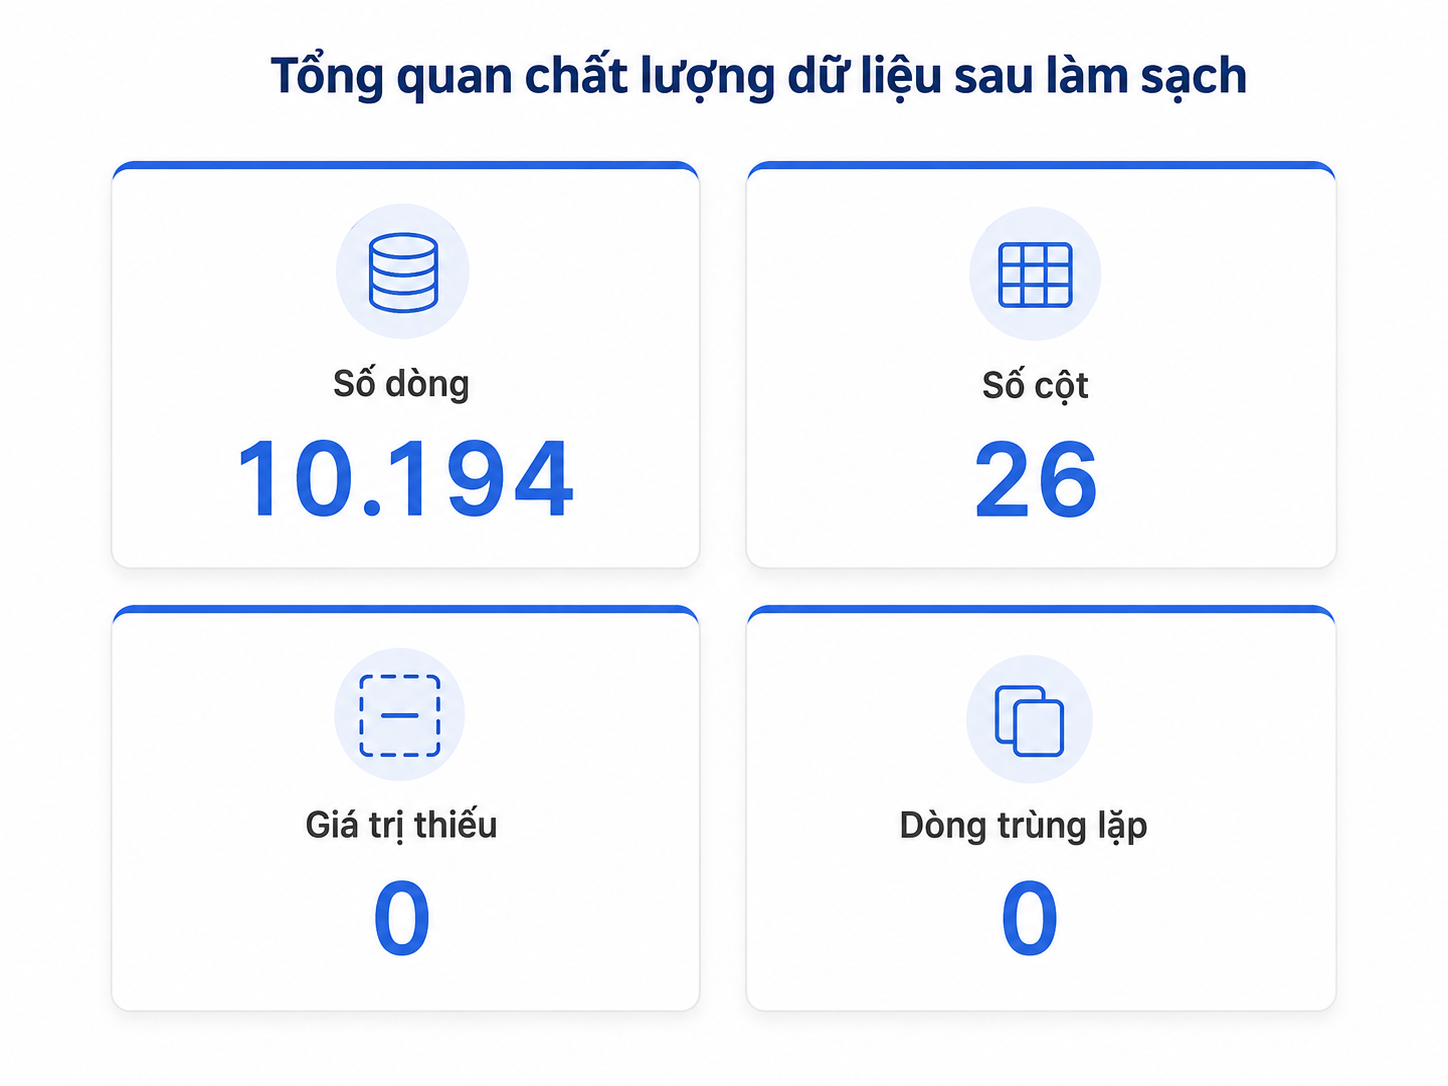
\includegraphics[width=0.85\textwidth]{images/anh_chuong3/hinh_3_8_tong_quan_chat_luong_du_lieu.png}
\caption{Tổng quan chất lượng dữ liệu sau làm sạch}
\label{fig:chat-luong-du-lieu}
\end{figure}

\refstepcounter{subsection}
\subsection*{\thesubsection\quad Thống kê mô tả các biến định lượng}

Thống kê mô tả là bước quan trọng trong phân tích khám phá dữ liệu, giúp tóm tắt đặc điểm phân bố của các biến và nhận diện những điểm đáng chú ý trong dữ liệu [1, 2]. Trong đồ án này, các biến định lượng chính gồm doanh thu, số lượng bán, chiết khấu và lợi nhuận. Bảng \ref{tab:thong-ke-mo-ta} trình bày thống kê mô tả của các biến này.

\begin{table}[H]
\centering
\caption{Thống kê mô tả các biến định lượng chính}
\label{tab:thong-ke-mo-ta}
\begin{tabular}{|l|r|r|r|r|}
\hline
\textbf{Biến} & \textbf{Trung bình} & \textbf{Trung vị} & \textbf{Nhỏ nhất} & \textbf{Lớn nhất} \\
\hline
Sales & 228,23 & 53,91 & 0,44 & 22.638,48 \\
\hline
Quantity & 3,79 & 3,00 & 1,00 & 14,00 \\
\hline
Discount & 0,16 & 0,20 & 0,00 & 0,80 \\
\hline
Profit & 28,67 & 8,69 & -6.599,98 & 8.399,98 \\
\hline
\end{tabular}
\end{table}

Kết quả thống kê cho thấy doanh thu trung bình của một dòng giao dịch là 228,23, trong khi trung vị chỉ đạt 53,91. Sự chênh lệch này cho thấy phân bố doanh thu có xu hướng lệch phải, tức là phần lớn giao dịch có giá trị nhỏ hoặc trung bình, trong khi một số giao dịch có giá trị rất lớn làm tăng giá trị trung bình. Lợi nhuận cũng có biên độ dao động lớn, từ -6.599,98 đến 8.399,98, phản ánh sự khác biệt đáng kể về hiệu quả kinh doanh giữa các giao dịch.

\refstepcounter{subsection}
\subsection*{\thesubsection\quad Phân tích tổng quan doanh thu, lợi nhuận và số lượng bán}

Tổng doanh thu của bộ dữ liệu đạt 2.326.534,35; tổng lợi nhuận đạt 292.296,81; tổng số lượng sản phẩm bán ra là 38.654. Ngoài ra, dữ liệu ghi nhận 1.901 dòng giao dịch có lợi nhuận âm với tổng mức lỗ là -157.038,93. Điều này cho thấy mặc dù hoạt động kinh doanh tổng thể có lãi, vẫn tồn tại một nhóm giao dịch gây lỗ cần được phân tích sâu hơn, đặc biệt khi xem xét theo danh mục sản phẩm, khu vực và mức chiết khấu.

\begin{table}[H]
\centering
\caption{Một số chỉ tiêu tổng quan về hoạt động kinh doanh}
\label{tab:kpi-tong-quan}
\begin{tabular}{|l|r|}
\hline
\textbf{Chỉ tiêu} & \textbf{Giá trị} \\
\hline
Tổng doanh thu & 2.326.534,35 \\
\hline
Tổng lợi nhuận & 292.296,81 \\
\hline
Tổng số lượng bán & 38.654 \\
\hline
Số đơn hàng & 5.111 \\
\hline
Số khách hàng & 804 \\
\hline
Số dòng có lợi nhuận âm & 1.901 \\
\hline
Tổng lỗ từ các dòng lợi nhuận âm & -157.038,93 \\
\hline
\end{tabular}
\end{table}

\refstepcounter{subsection}
\subsection*{\thesubsection\quad Phân tích doanh thu và lợi nhuận theo thời gian}

Phân tích theo thời gian giúp nhận diện xu hướng biến động của doanh số và lợi nhuận trong từng giai đoạn. Đây là nội dung trực tiếp trả lời câu hỏi nghiên cứu: doanh số bán hàng thay đổi như thế nào theo thời gian. Kết quả tổng hợp theo năm được trình bày trong Bảng \ref{tab:theo-nam}.

\begin{table}[H]
\centering
\caption{Doanh thu, lợi nhuận và số lượng bán theo năm}
\label{tab:theo-nam}
\begin{tabular}{|r|r|r|r|r|}
\hline
\textbf{Năm} & \textbf{Doanh thu} & \textbf{Lợi nhuận} & \textbf{Số lượng bán} & \textbf{Số đơn hàng} \\
\hline
2023 & 494.040,21 & 51.684,30 & 7.813 & 995 \\
\hline
2024 & 472.993,03 & 62.020,97 & 8.086 & 1.053 \\
\hline
2025 & 613.933,58 & 82.665,20 & 10.018 & 1.340 \\
\hline
2026 & 745.567,53 & 95.926,35 & 12.737 & 1.723 \\
\hline
\end{tabular}
\end{table}

Từ Bảng \ref{tab:theo-nam}, có thể thấy doanh thu và lợi nhuận nhìn chung có xu hướng tăng qua các năm. Năm 2026 là năm có doanh thu cao nhất với 745.567,53 và lợi nhuận cao nhất với 95.926,35. Số đơn hàng và số lượng bán cũng tăng mạnh trong năm 2026, cho thấy quy mô hoạt động kinh doanh được mở rộng so với các năm trước.

\begin{figure}[H]
\centering
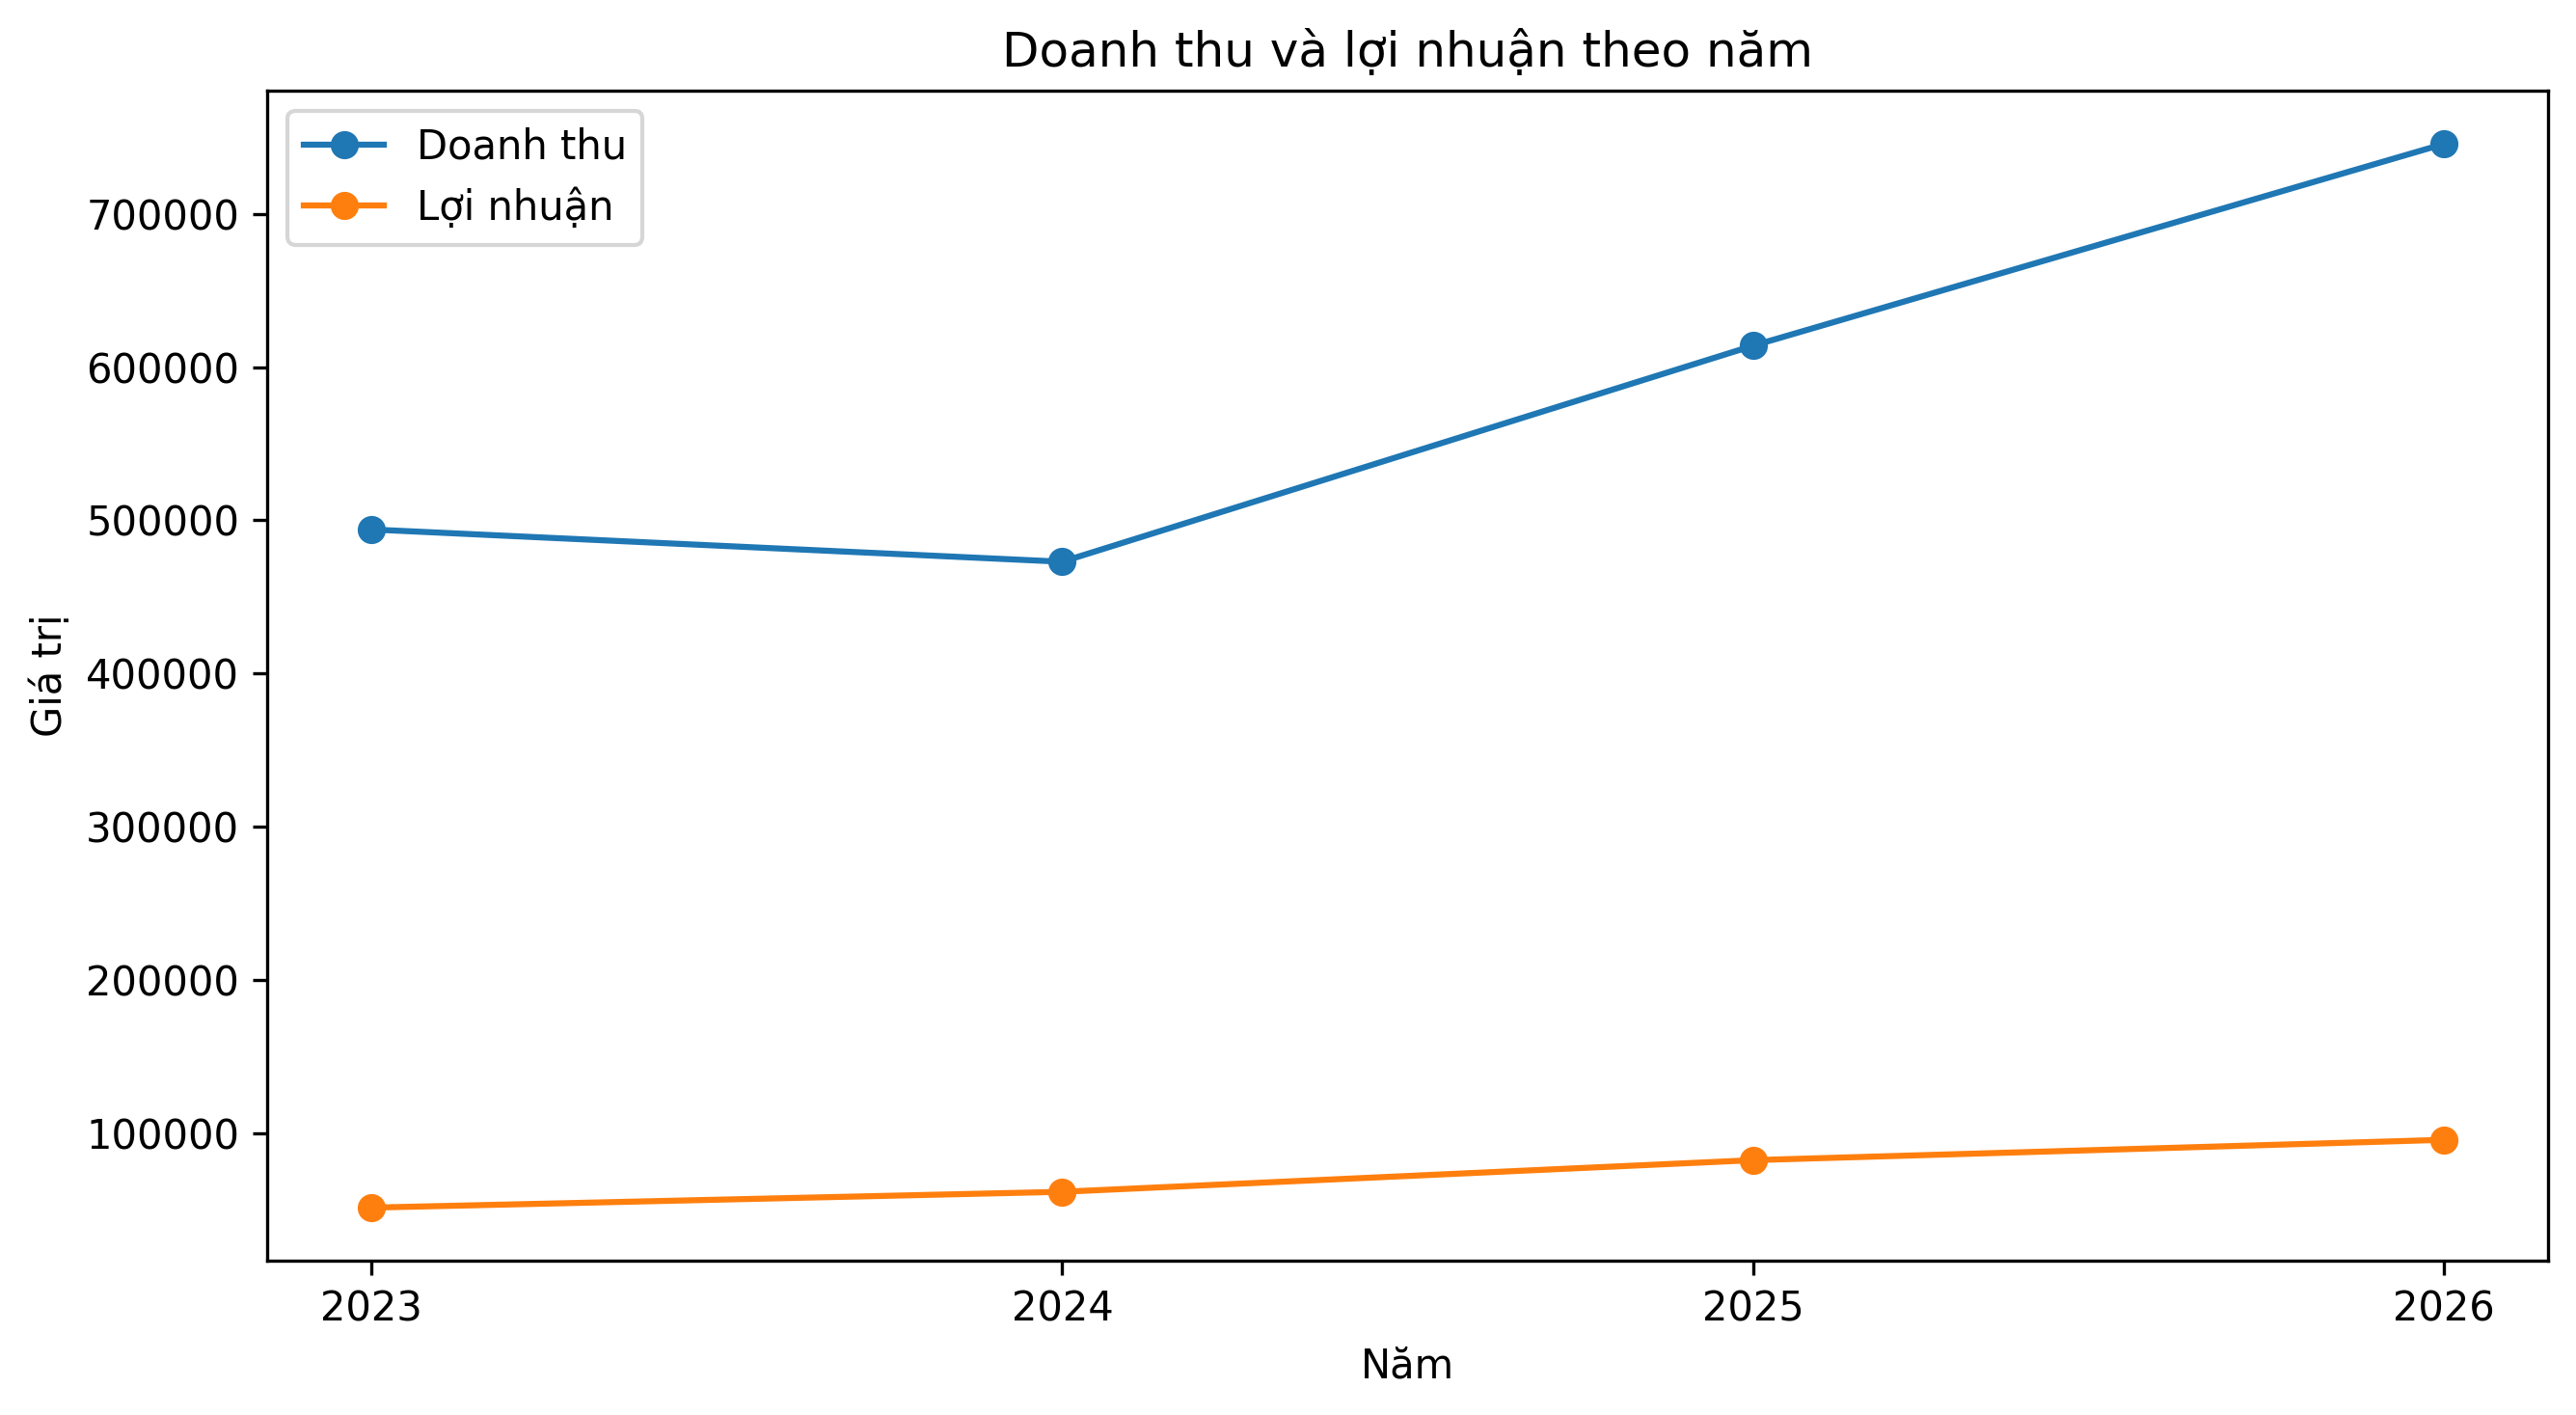
\includegraphics[width=0.9\textwidth]{images/anh_chuong3/hinh_3_1_doanh_thu_loi_nhuan_theo_nam.png}
\caption{Doanh thu và lợi nhuận theo năm}
\label{fig:doanh-thu-loi-nhuan-nam}
\end{figure}

Bên cạnh xu hướng theo năm, việc quan sát doanh thu theo tháng giúp nhận diện rõ hơn mức độ dao động trong từng giai đoạn. Hình \ref{fig:xu-huong-thang} thể hiện xu hướng doanh thu theo tháng trong toàn bộ giai đoạn nghiên cứu.

\begin{figure}[H]
\centering
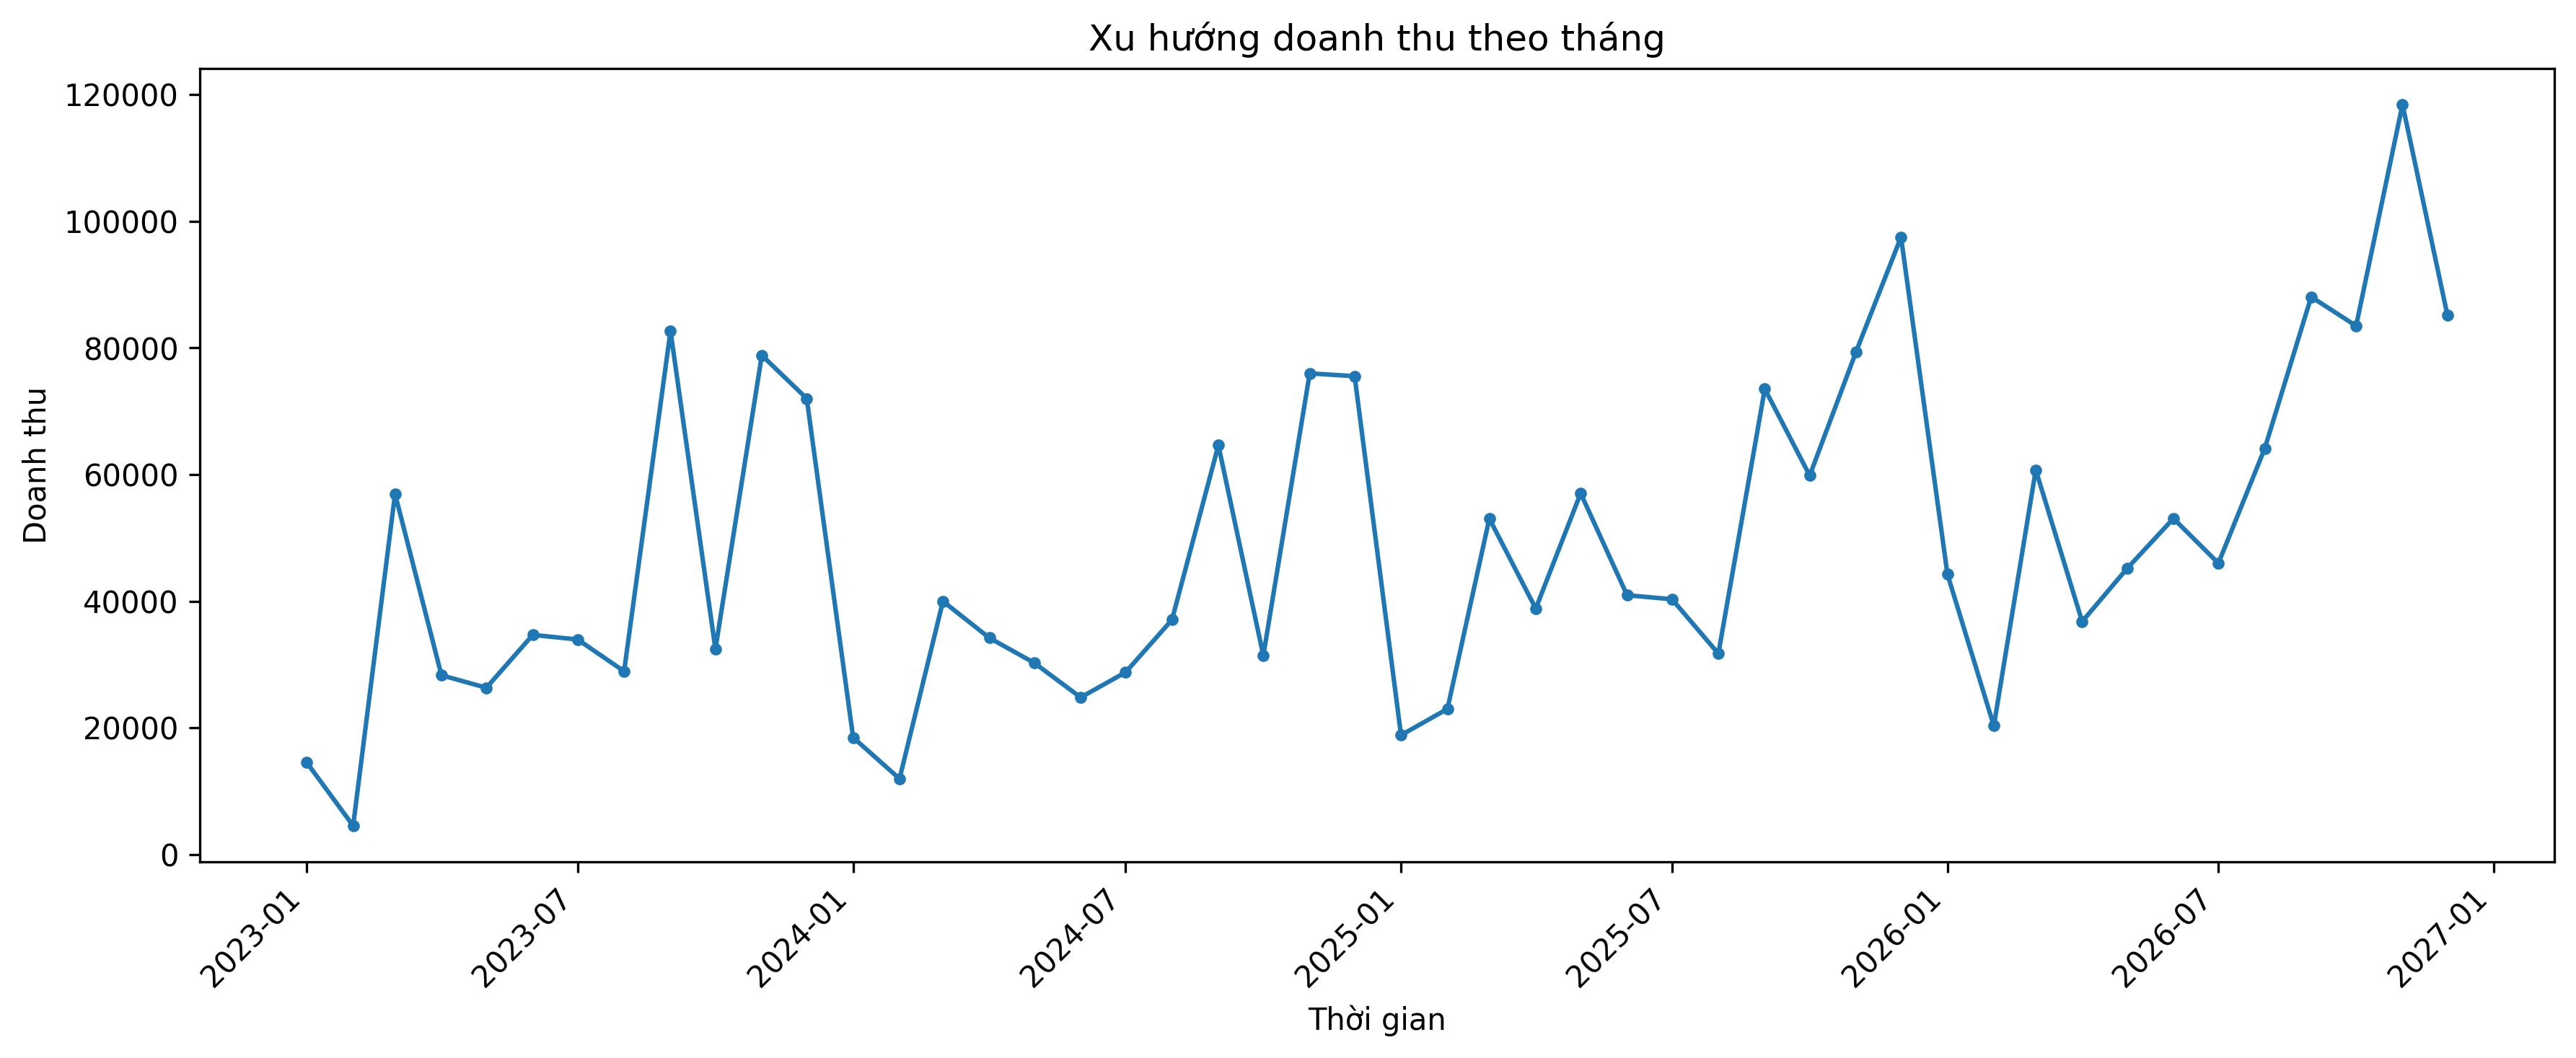
\includegraphics[width=0.95\textwidth]{images/anh_chuong3/hinh_3_7_xu_huong_doanh_thu_theo_thang.png}
\caption{Xu hướng doanh thu theo tháng}
\label{fig:xu-huong-thang}
\end{figure}

\refstepcounter{subsection}
\subsection*{\thesubsection\quad Phân tích theo khu vực bán hàng}

Phân tích theo khu vực giúp đánh giá mức độ đóng góp của từng vùng vào kết quả kinh doanh. Kết quả cho thấy khu vực West đạt doanh thu và lợi nhuận cao nhất, tiếp theo là East. Trong khi đó, South có doanh thu thấp nhất nhưng lợi nhuận vẫn cao hơn Central. Điều này cho thấy hiệu quả kinh doanh không chỉ phụ thuộc vào quy mô doanh thu mà còn chịu ảnh hưởng bởi cơ cấu sản phẩm, chiết khấu và khả năng sinh lợi của từng khu vực.

\begin{table}[H]
\centering
\caption{Doanh thu và lợi nhuận theo khu vực}
\label{tab:khu-vuc}
\begin{tabular}{|l|r|r|r|}
\hline
\textbf{Khu vực} & \textbf{Doanh thu} & \textbf{Lợi nhuận} & \textbf{Số đơn hàng} \\
\hline
West & 739.813,61 & 110.798,82 & 1.635 \\
\hline
East & 691.828,17 & 94.883,26 & 1.475 \\
\hline
Central & 503.170,67 & 39.865,31 & 1.179 \\
\hline
South & 391.721,91 & 46.749,43 & 822 \\
\hline
\end{tabular}
\end{table}

\begin{figure}[H]
\centering
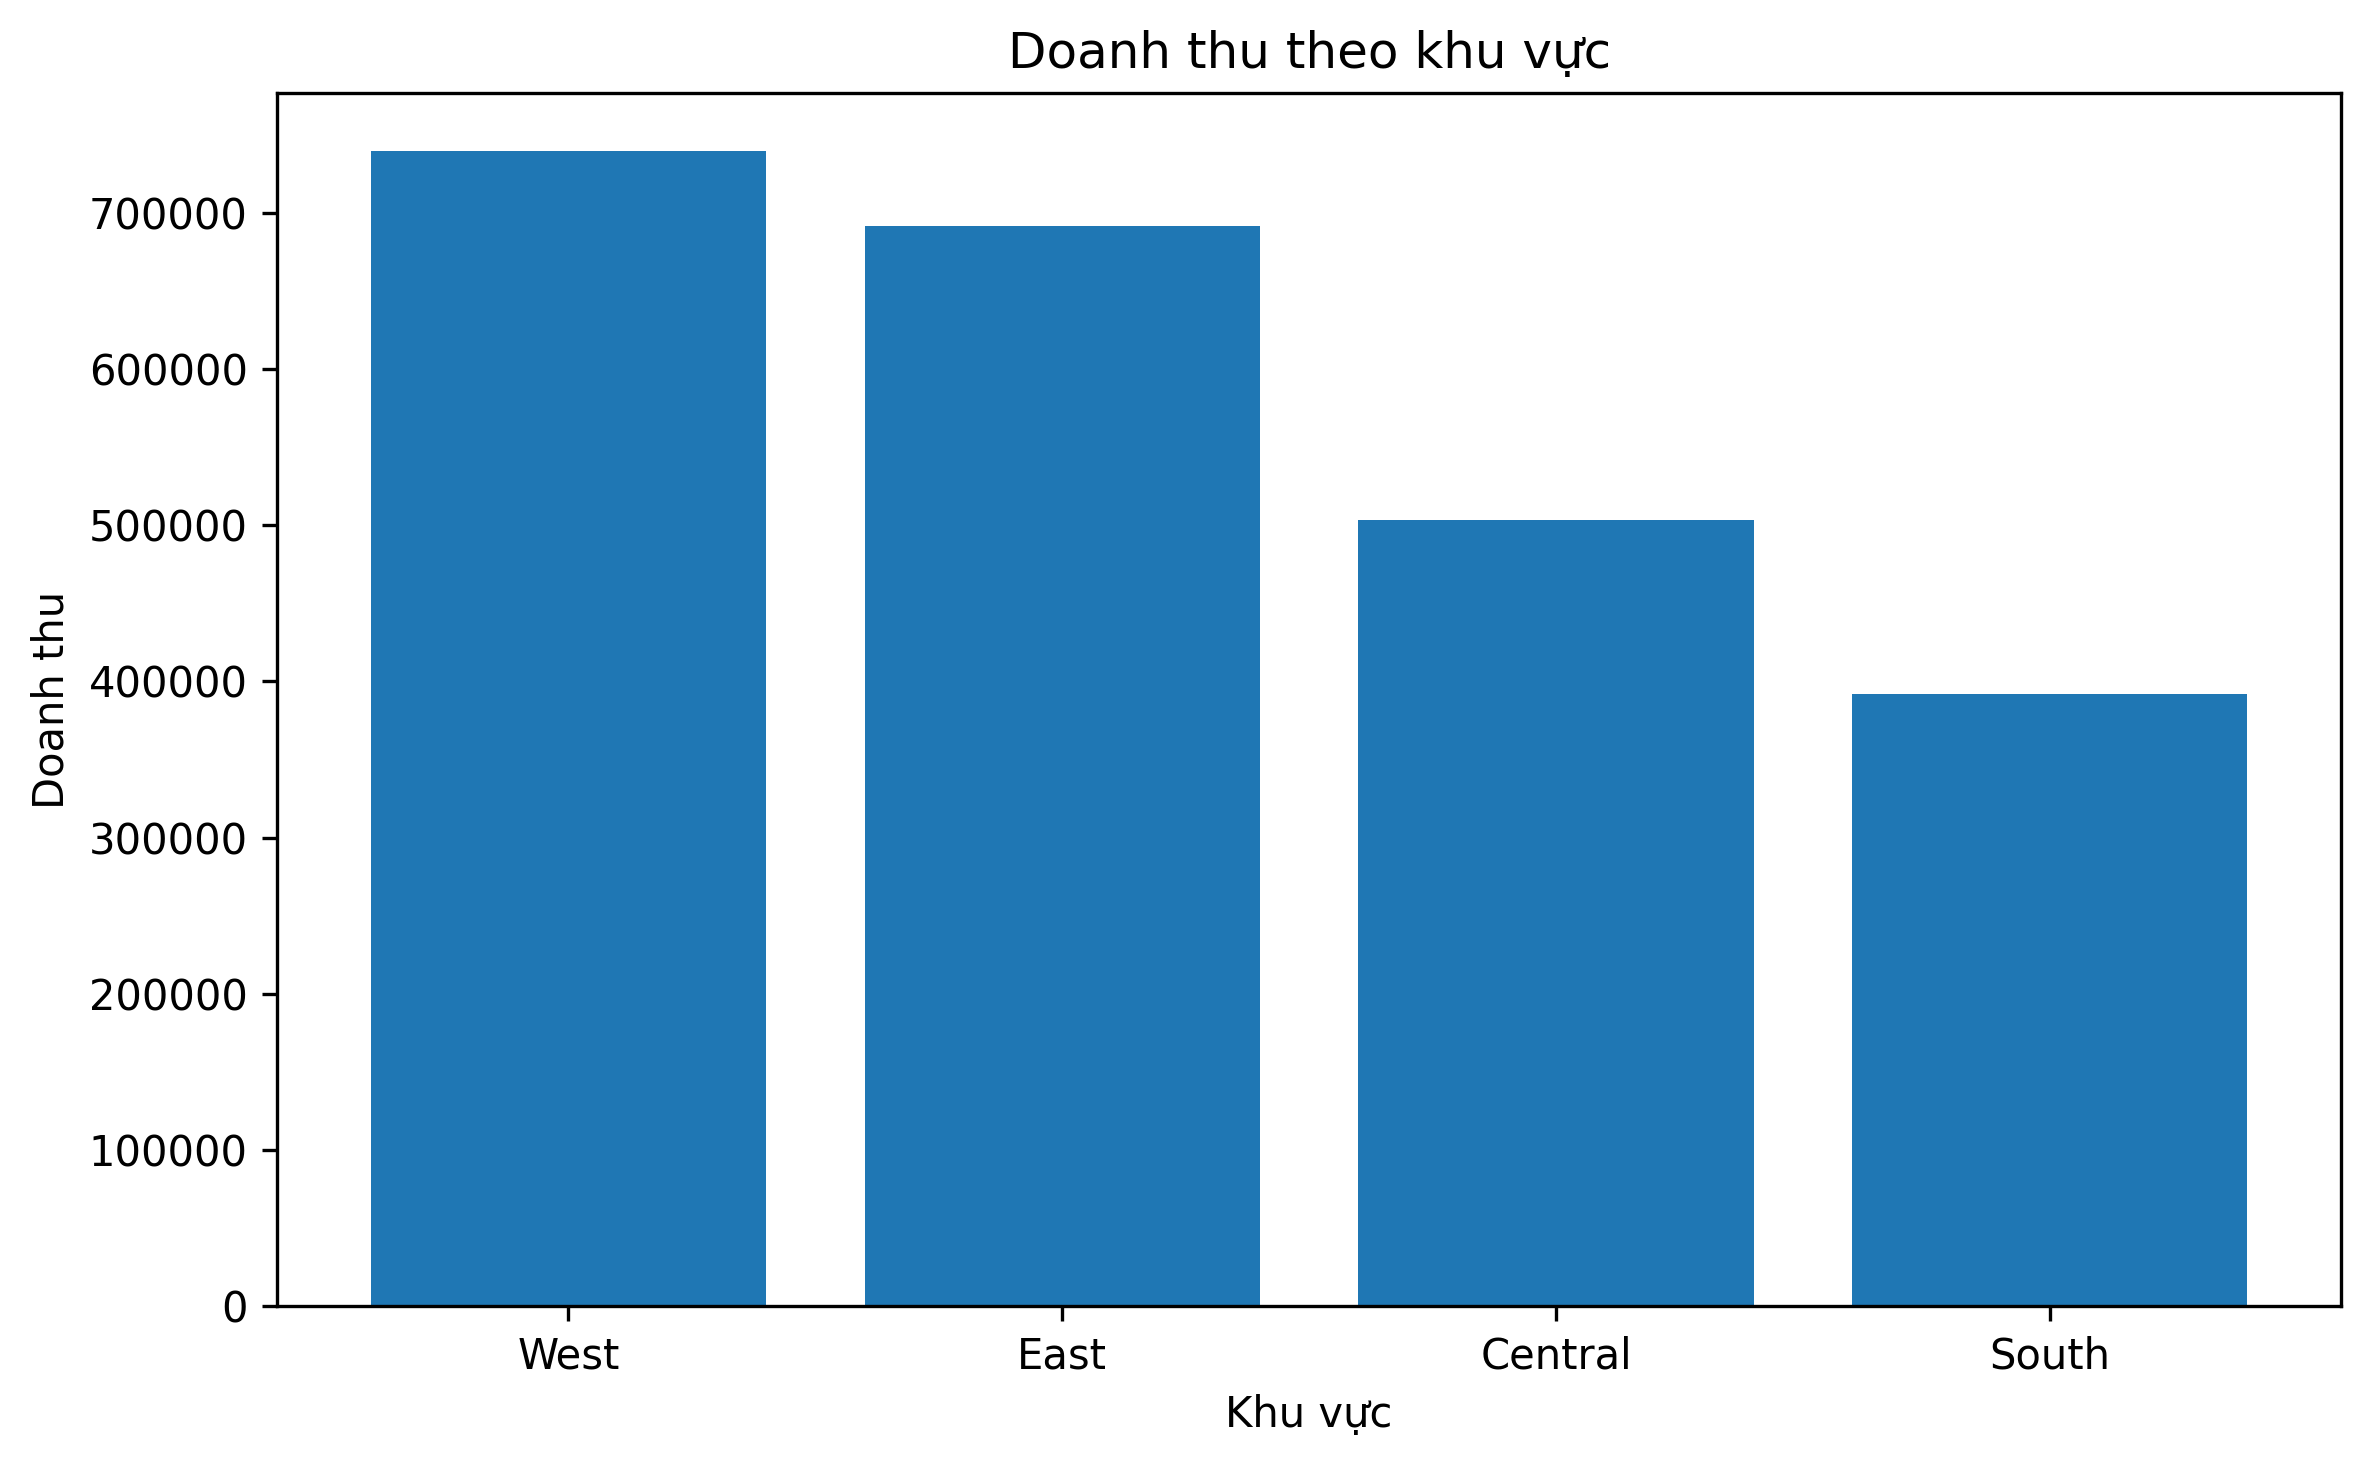
\includegraphics[width=0.85\textwidth]{images/anh_chuong3/hinh_3_2_doanh_thu_theo_khu_vuc.png}
\caption{Doanh thu theo khu vực}
\label{fig:doanh-thu-khu-vuc}
\end{figure}

\refstepcounter{subsection}
\subsection*{\thesubsection\quad Phân tích theo danh mục và tiểu danh mục sản phẩm}

Phân tích theo danh mục sản phẩm giúp xác định nhóm sản phẩm đóng góp chính vào doanh thu và lợi nhuận. Kết quả cho thấy Technology là danh mục có doanh thu và lợi nhuận cao nhất, với lợi nhuận đạt 146.543,38. Office Supplies có lợi nhuận cao thứ hai, trong khi Furniture tuy có doanh thu lớn nhưng lợi nhuận chỉ đạt 19.730,00. Điều này cho thấy Furniture có hiệu quả sinh lời thấp hơn so với hai danh mục còn lại.

\begin{table}[H]
\centering
\caption{Doanh thu, lợi nhuận và số lượng bán theo danh mục sản phẩm}
\label{tab:danh-muc}
\begin{tabular}{|l|r|r|r|}
\hline
\textbf{Danh mục} & \textbf{Doanh thu} & \textbf{Lợi nhuận} & \textbf{Số lượng bán} \\
\hline
Technology & 839.893,28 & 146.543,38 & 7.017 \\
\hline
Furniture & 754.747,76 & 19.730,00 & 8.369 \\
\hline
Office Supplies & 731.893,31 & 126.023,44 & 23.268 \\
\hline
\end{tabular}
\end{table}

\begin{figure}[H]
\centering
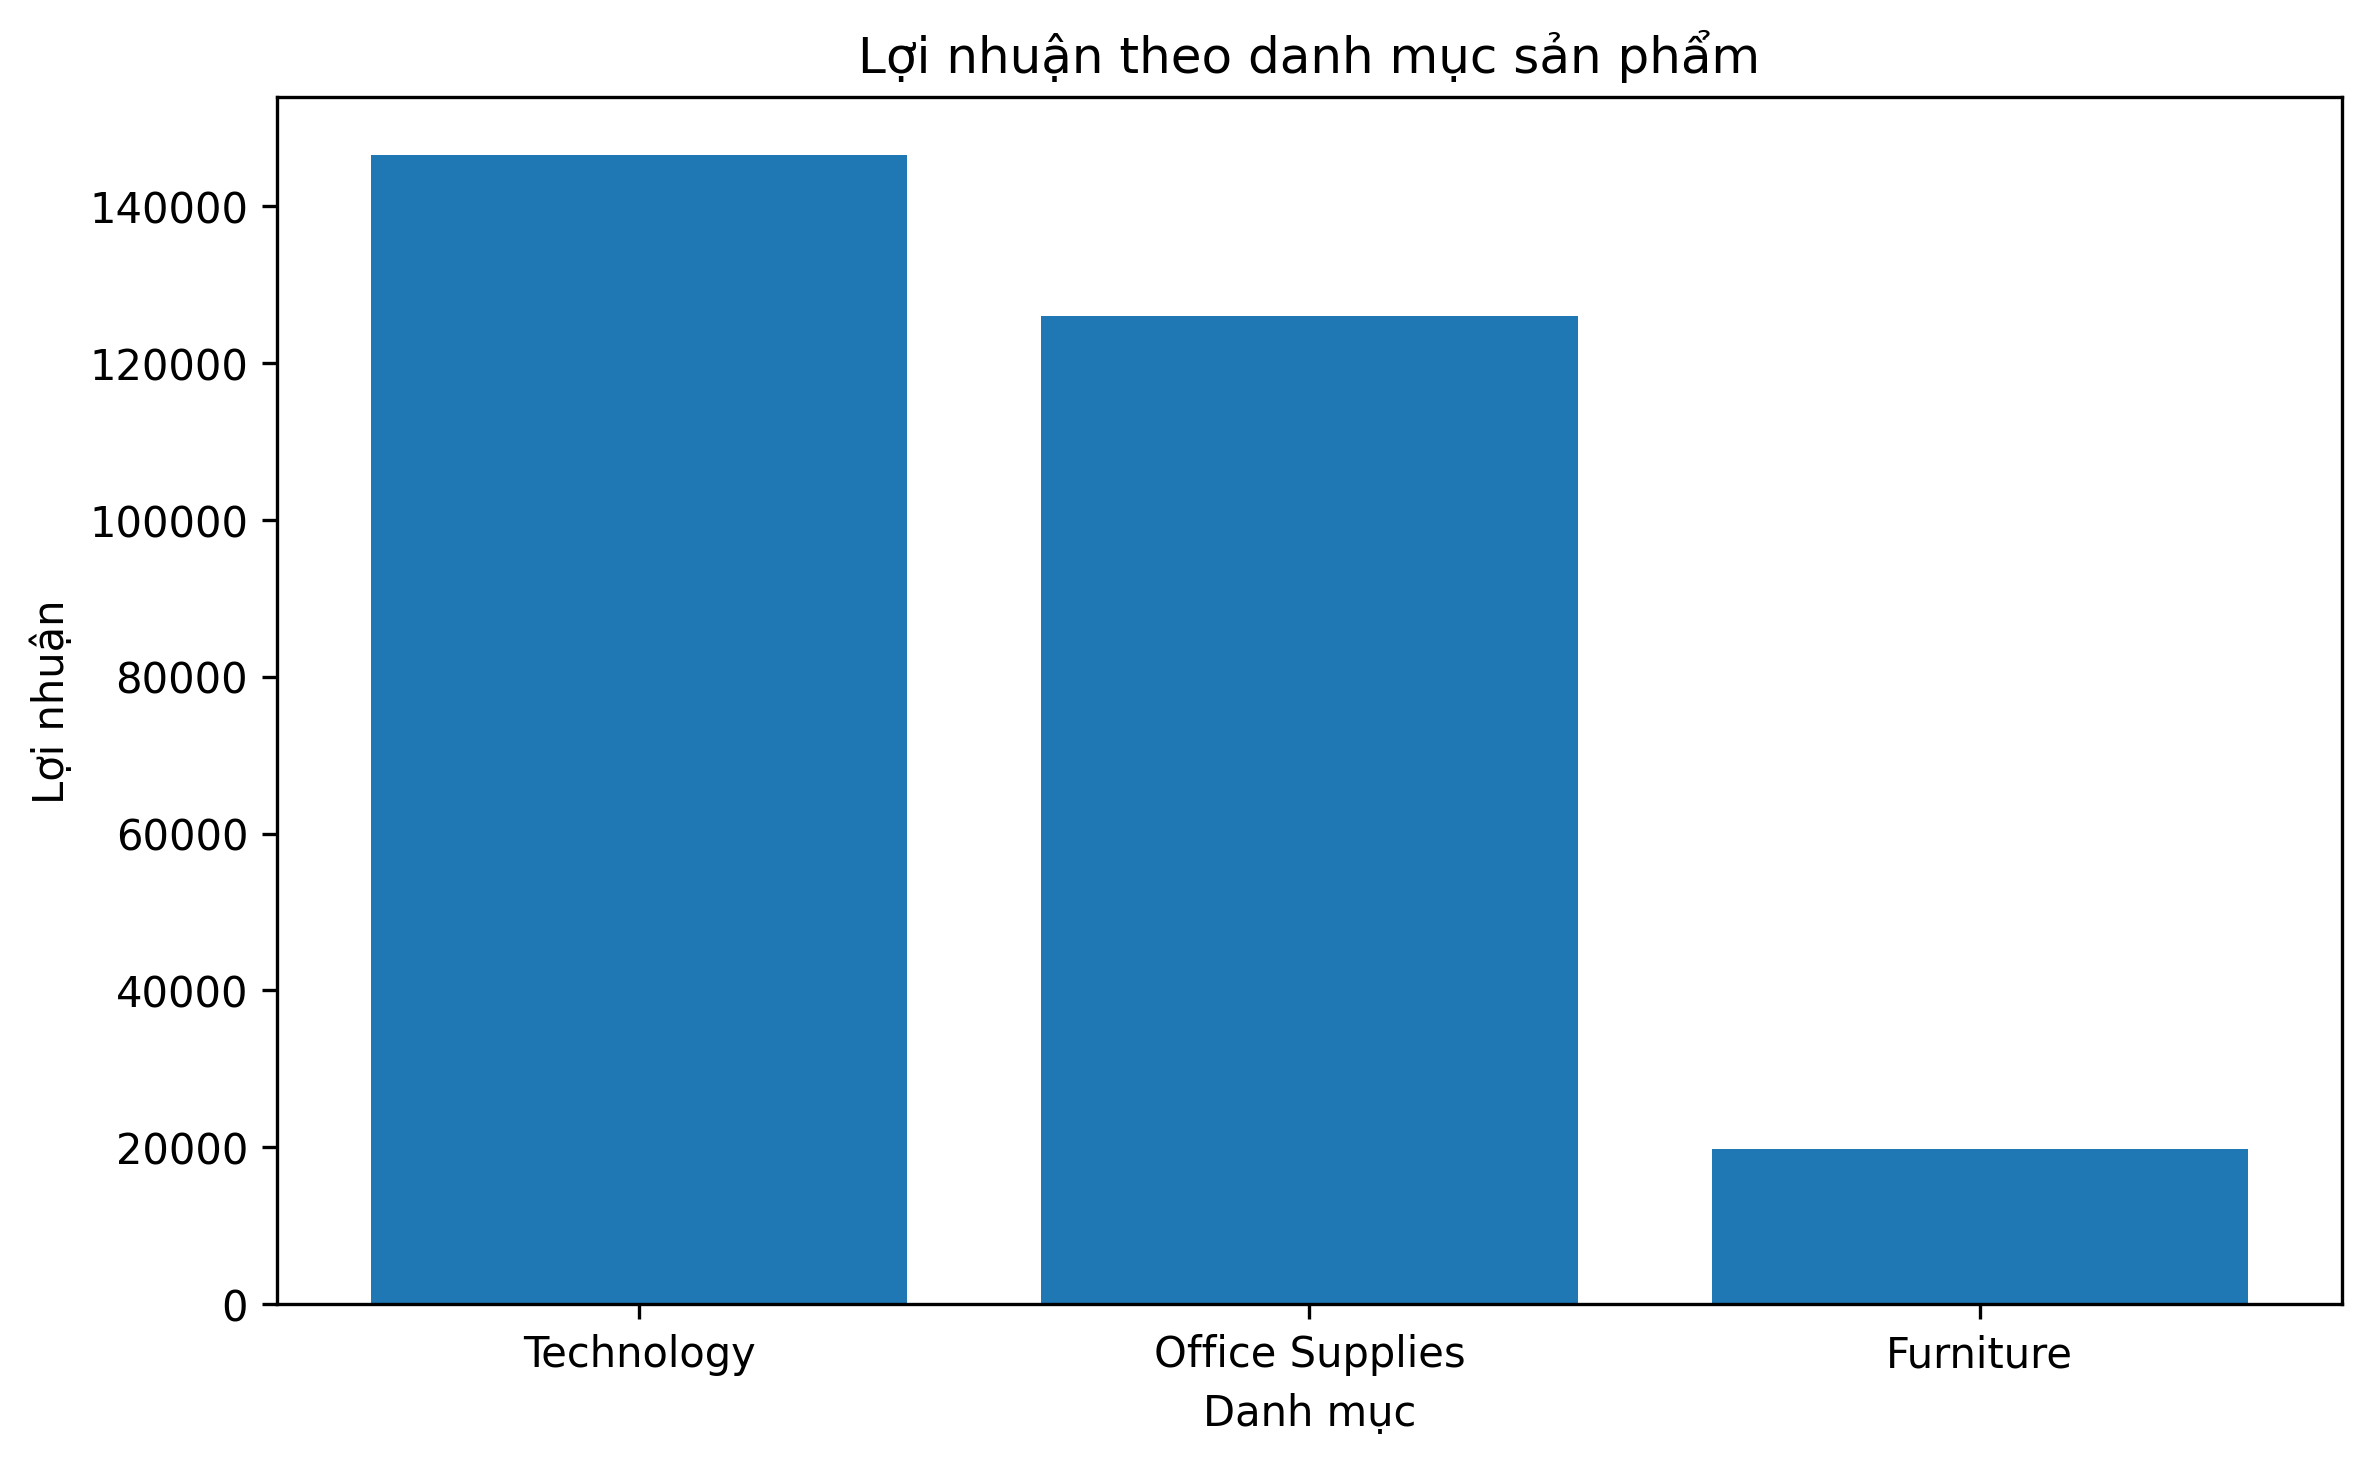
\includegraphics[width=0.85\textwidth]{images/anh_chuong3/hinh_3_3_loi_nhuan_theo_danh_muc.png}
\caption{Lợi nhuận theo danh mục sản phẩm}
\label{fig:loi-nhuan-danh-muc}
\end{figure}

Ở cấp tiểu danh mục, Copiers, Phones, Accessories và Paper là những nhóm có lợi nhuận cao. Ngược lại, Tables, Bookcases và Supplies là các tiểu danh mục có lợi nhuận âm. Đây là thông tin quan trọng để đánh giá hiệu quả kinh doanh theo từng nhóm sản phẩm cụ thể.

\begin{table}[H]
\centering
\caption{Top 5 tiểu danh mục có lợi nhuận cao nhất}
\label{tab:top-subcategory}
\begin{tabular}{|l|r|r|}
\hline
\textbf{Tiểu danh mục} & \textbf{Doanh thu} & \textbf{Lợi nhuận} \\
\hline
Copiers & 150.745,29 & 56.093,94 \\
\hline
Phones & 331.842,64 & 45.050,83 \\
\hline
Accessories & 167.380,32 & 41.936,64 \\
\hline
Paper & 79.540,54 & 34.511,51 \\
\hline
Binders & 207.354,88 & 31.426,10 \\
\hline
\end{tabular}
\end{table}

\begin{figure}[H]
\centering
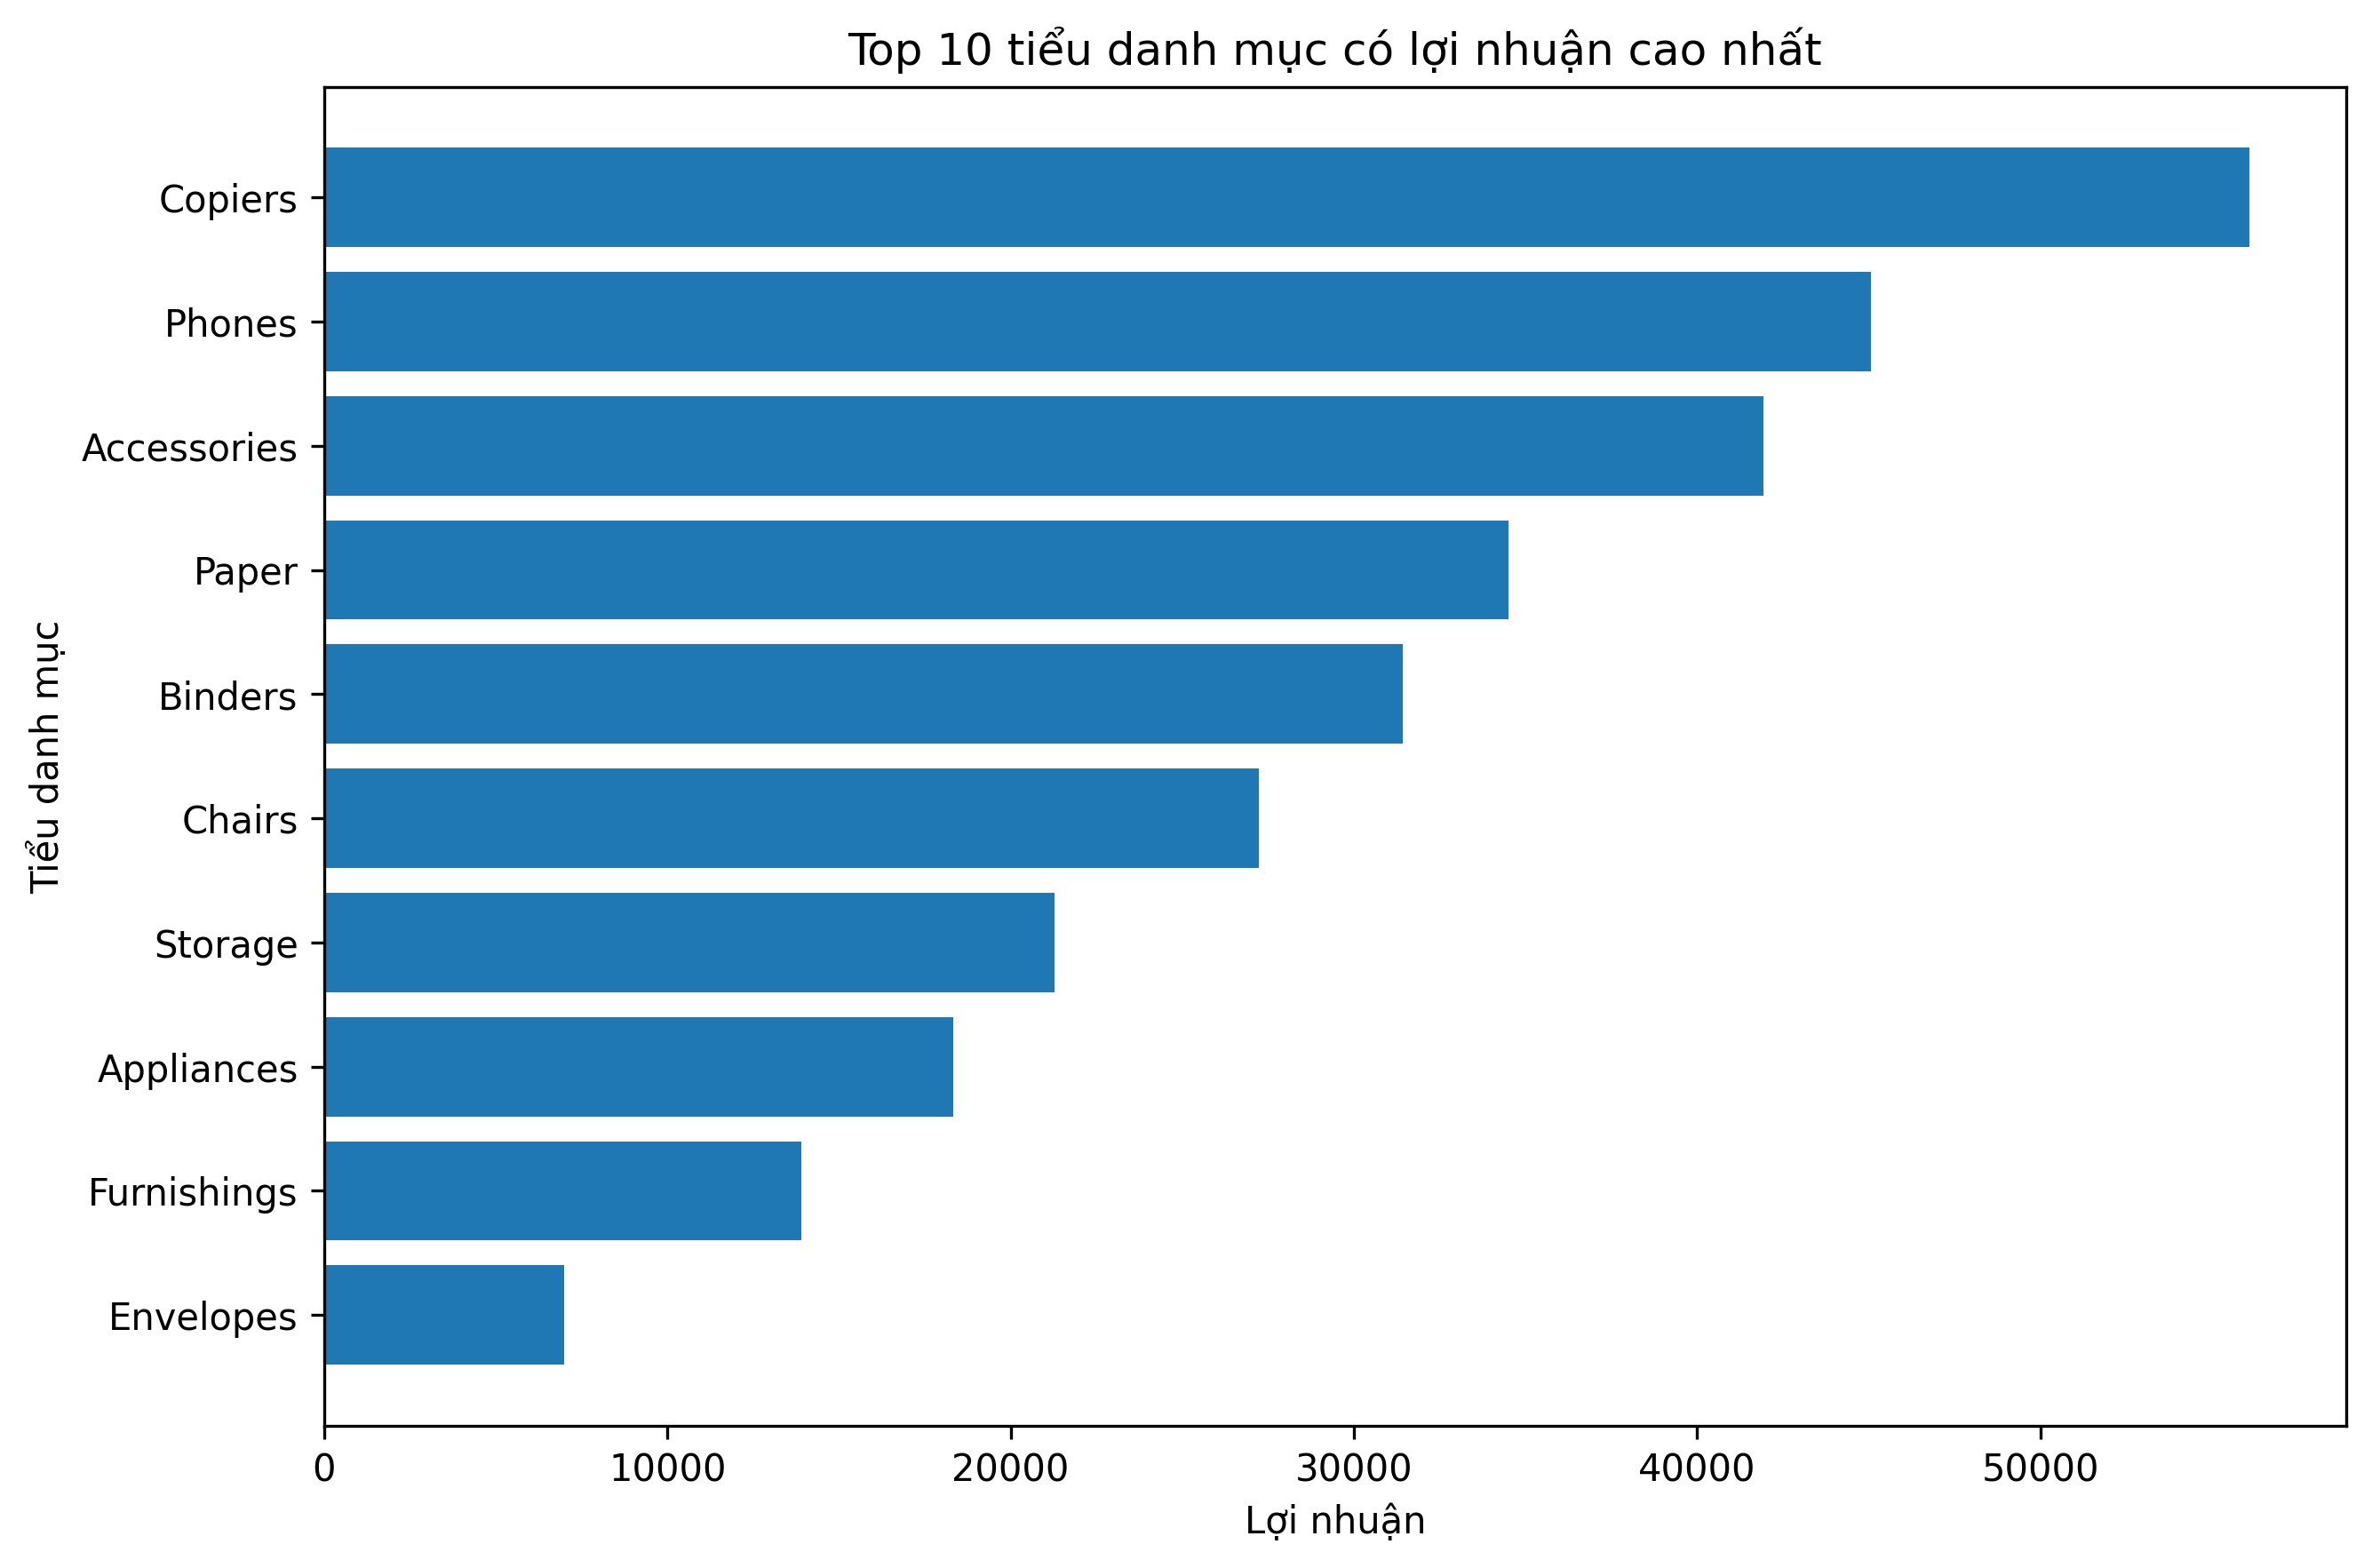
\includegraphics[width=0.9\textwidth]{images/anh_chuong3/hinh_3_4_top_10_tieu_danh_muc_loi_nhuan.png}
\caption{Top 10 tiểu danh mục có lợi nhuận cao nhất}
\label{fig:top-subcategory}
\end{figure}

\refstepcounter{subsection}
\subsection*{\thesubsection\quad Phân tích theo phân khúc khách hàng}

Phân khúc khách hàng là biến quan trọng để nhận diện xu hướng tiêu dùng của từng nhóm đối tượng. Kết quả tổng hợp cho thấy nhóm Consumer đóng góp doanh thu cao nhất với 1.170.660,25 và lợi nhuận cao nhất với 136.371,45. Nhóm Corporate đứng thứ hai, trong khi Home Office có quy mô doanh thu nhỏ hơn nhưng vẫn tạo ra lợi nhuận đáng kể.

\begin{table}[H]
\centering
\caption{Doanh thu và lợi nhuận theo phân khúc khách hàng}
\label{tab:phan-khuc}
\begin{tabular}{|l|r|r|r|r|}
\hline
\textbf{Phân khúc} & \textbf{Doanh thu} & \textbf{Lợi nhuận} & \textbf{Số đơn hàng} & \textbf{Số khách hàng} \\
\hline
Consumer & 1.170.660,25 & 136.371,45 & 2.628 & 416 \\
\hline
Corporate & 715.806,12 & 94.249,64 & 1.552 & 239 \\
\hline
Home Office & 440.067,98 & 61.675,73 & 931 & 149 \\
\hline
\end{tabular}
\end{table}

\begin{figure}[H]
\centering
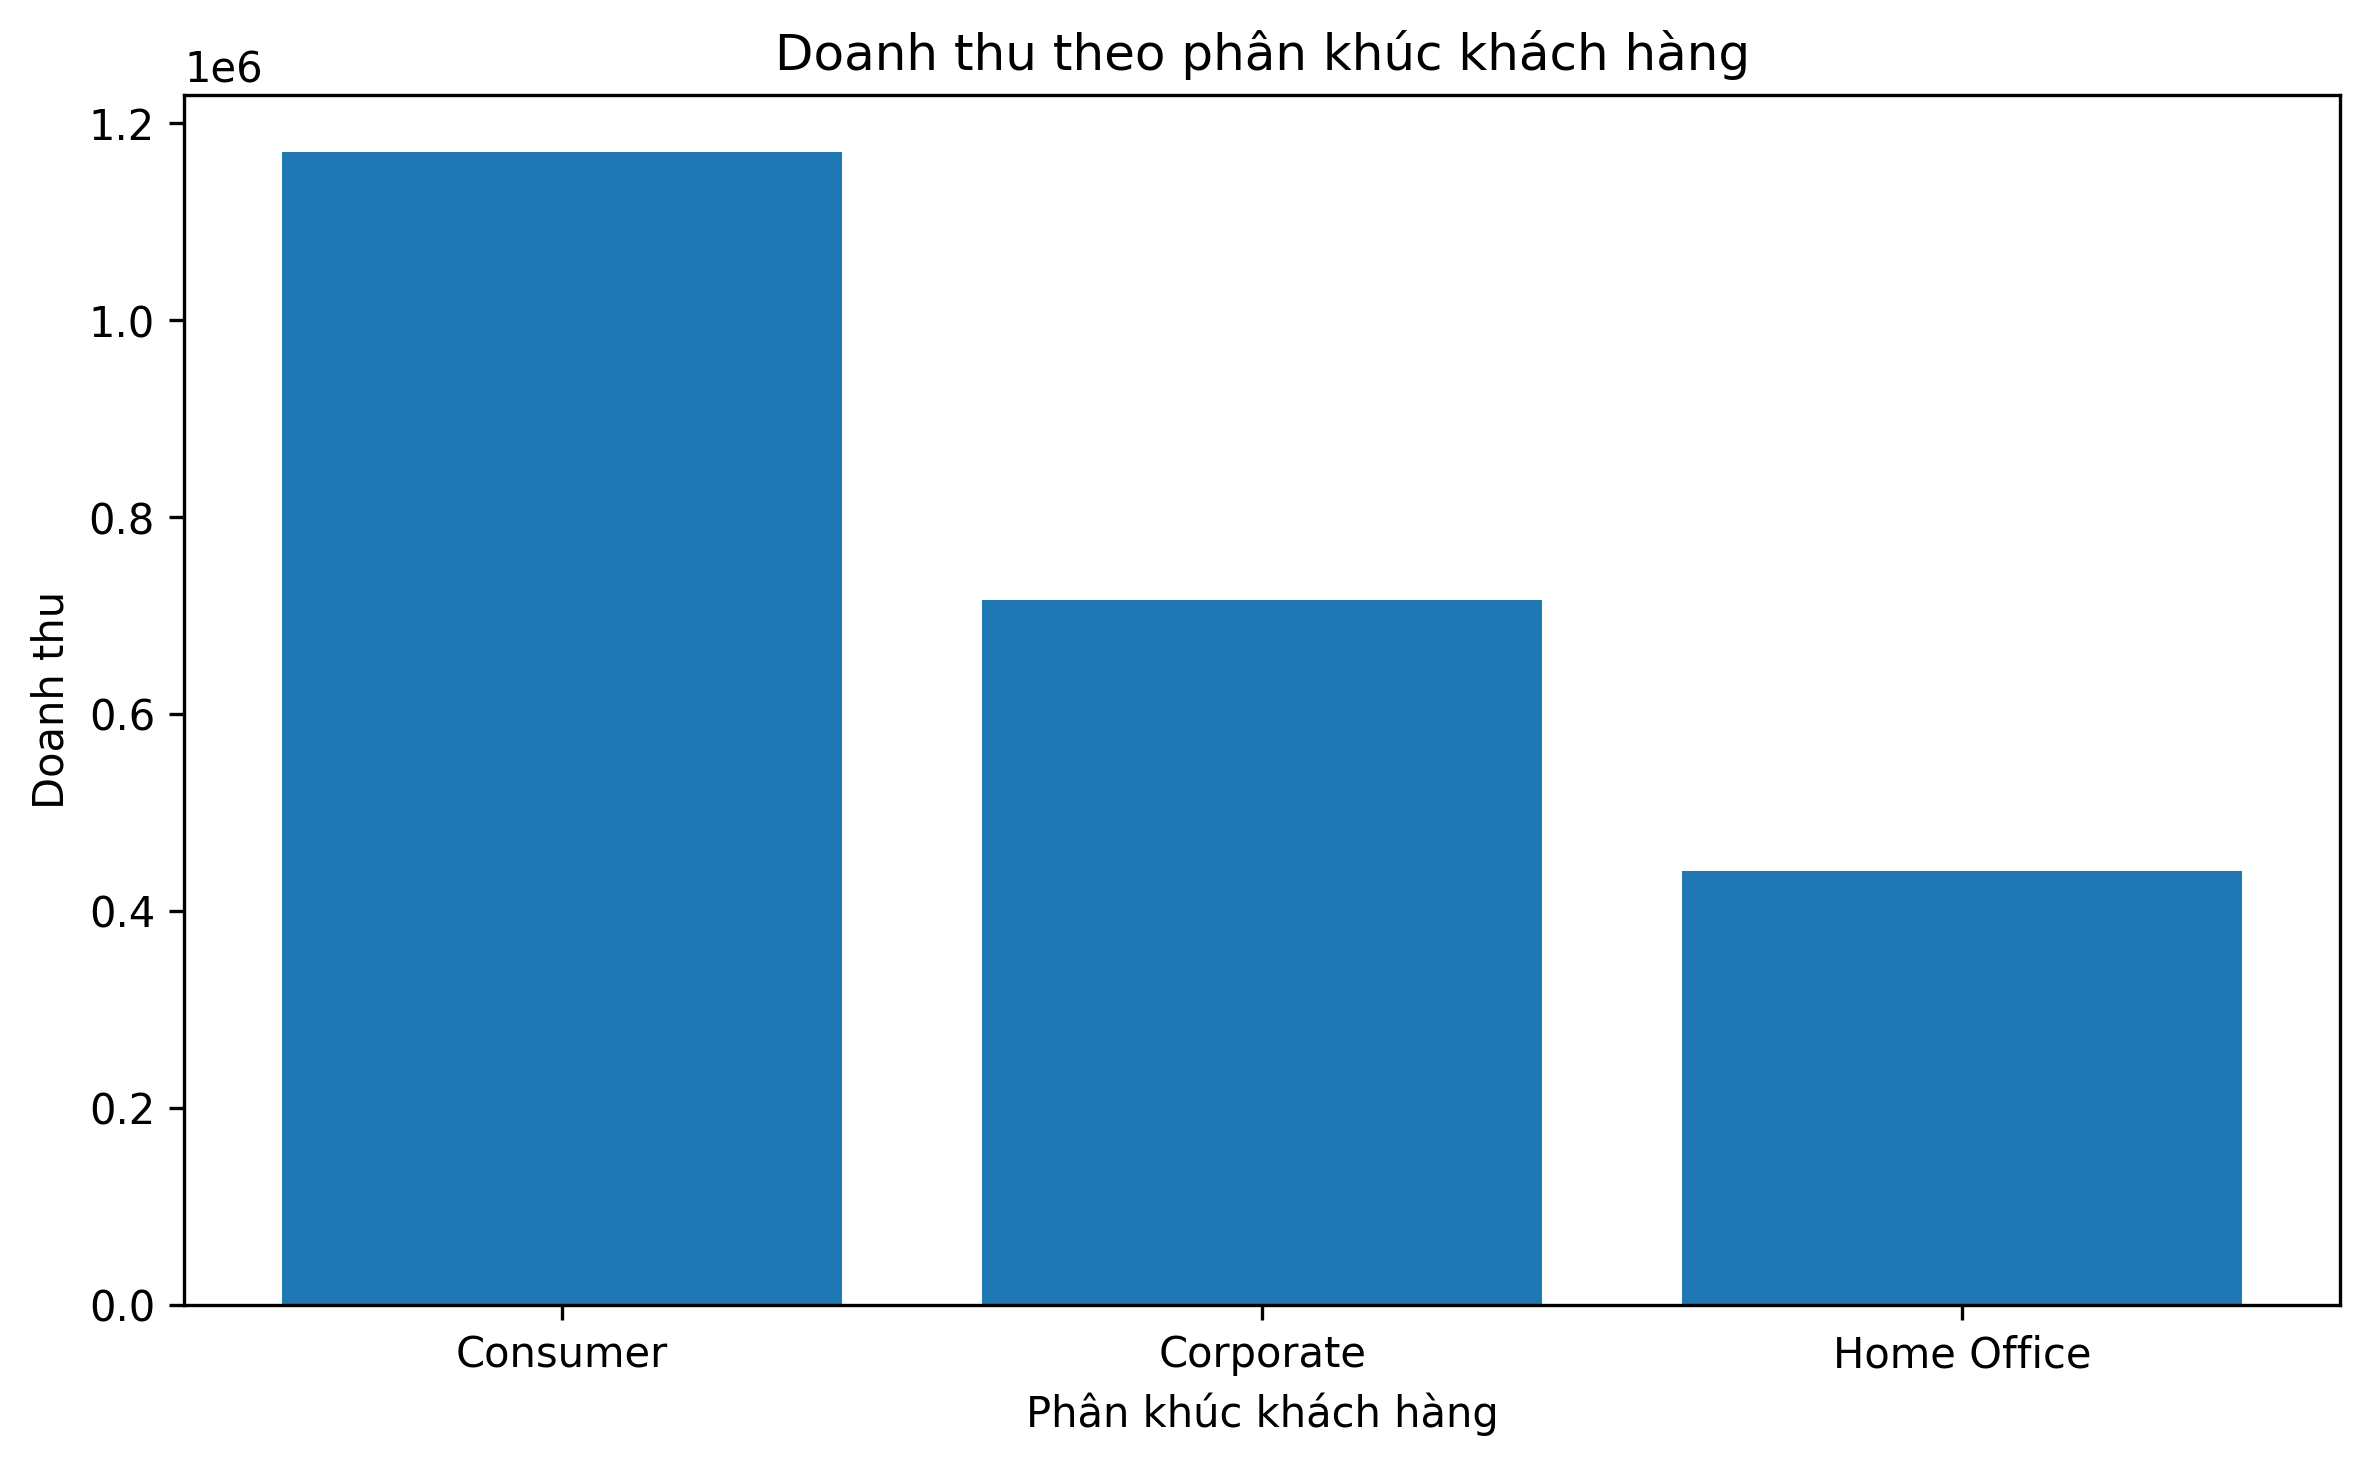
\includegraphics[width=0.85\textwidth]{images/anh_chuong3/hinh_3_5_doanh_thu_theo_phan_khuc.png}
\caption{Doanh thu theo phân khúc khách hàng}
\label{fig:doanh-thu-phan-khuc}
\end{figure}

Kết quả này cho thấy nhóm Consumer là nhóm khách hàng có xu hướng tiêu dùng cao nhất xét theo tổng doanh thu. Tuy nhiên, để đánh giá sâu hơn giá trị của từng nhóm khách hàng, cần kết hợp thêm các chỉ tiêu như lợi nhuận, số đơn hàng, giá trị trung bình mỗi đơn hàng và tần suất mua hàng.

\refstepcounter{subsection}
\subsection*{\thesubsection\quad Phân tích ảnh hưởng của chiết khấu đến lợi nhuận}

Chiết khấu là một yếu tố quan trọng trong hoạt động bán hàng vì có thể kích thích tiêu dùng nhưng đồng thời cũng làm giảm biên lợi nhuận. Vì vậy, việc phân tích mối quan hệ giữa chiết khấu và lợi nhuận giúp đánh giá hiệu quả của chính sách giảm giá. Theo kết quả tổng hợp, các nhóm chiết khấu thấp từ 0--20\% vẫn tạo ra lợi nhuận dương, trong khi các nhóm chiết khấu từ 20\% trở lên bắt đầu ghi nhận lợi nhuận âm ở nhiều mức khác nhau.

\begin{table}[H]
\centering
\caption{Lợi nhuận theo nhóm chiết khấu}
\label{tab:chiet-khau}
\begin{tabular}{|l|r|r|r|}
\hline
\textbf{Nhóm chiết khấu} & \textbf{Doanh thu} & \textbf{Lợi nhuận} & \textbf{Số dòng} \\
\hline
0--10\% & 1.160.275,60 & 335.818,56 & 5.021 \\
\hline
10--20\% & 801.497,85 & 92.498,94 & 3.758 \\
\hline
20--30\% & 104.474,07 & -10.513,45 & 230 \\
\hline
30--40\% & 130.991,18 & -25.477,51 & 234 \\
\hline
40--50\% & 64.403,51 & -22.999,54 & 77 \\
\hline
50--60\% & 7.105,94 & -6.164,35 & 149 \\
\hline
60--70\% & 40.805,27 & -40.300,57 & 424 \\
\hline
70--80\% & 16.980,15 & -30.565,27 & 301 \\
\hline
\end{tabular}
\end{table}

\begin{figure}[H]
\centering
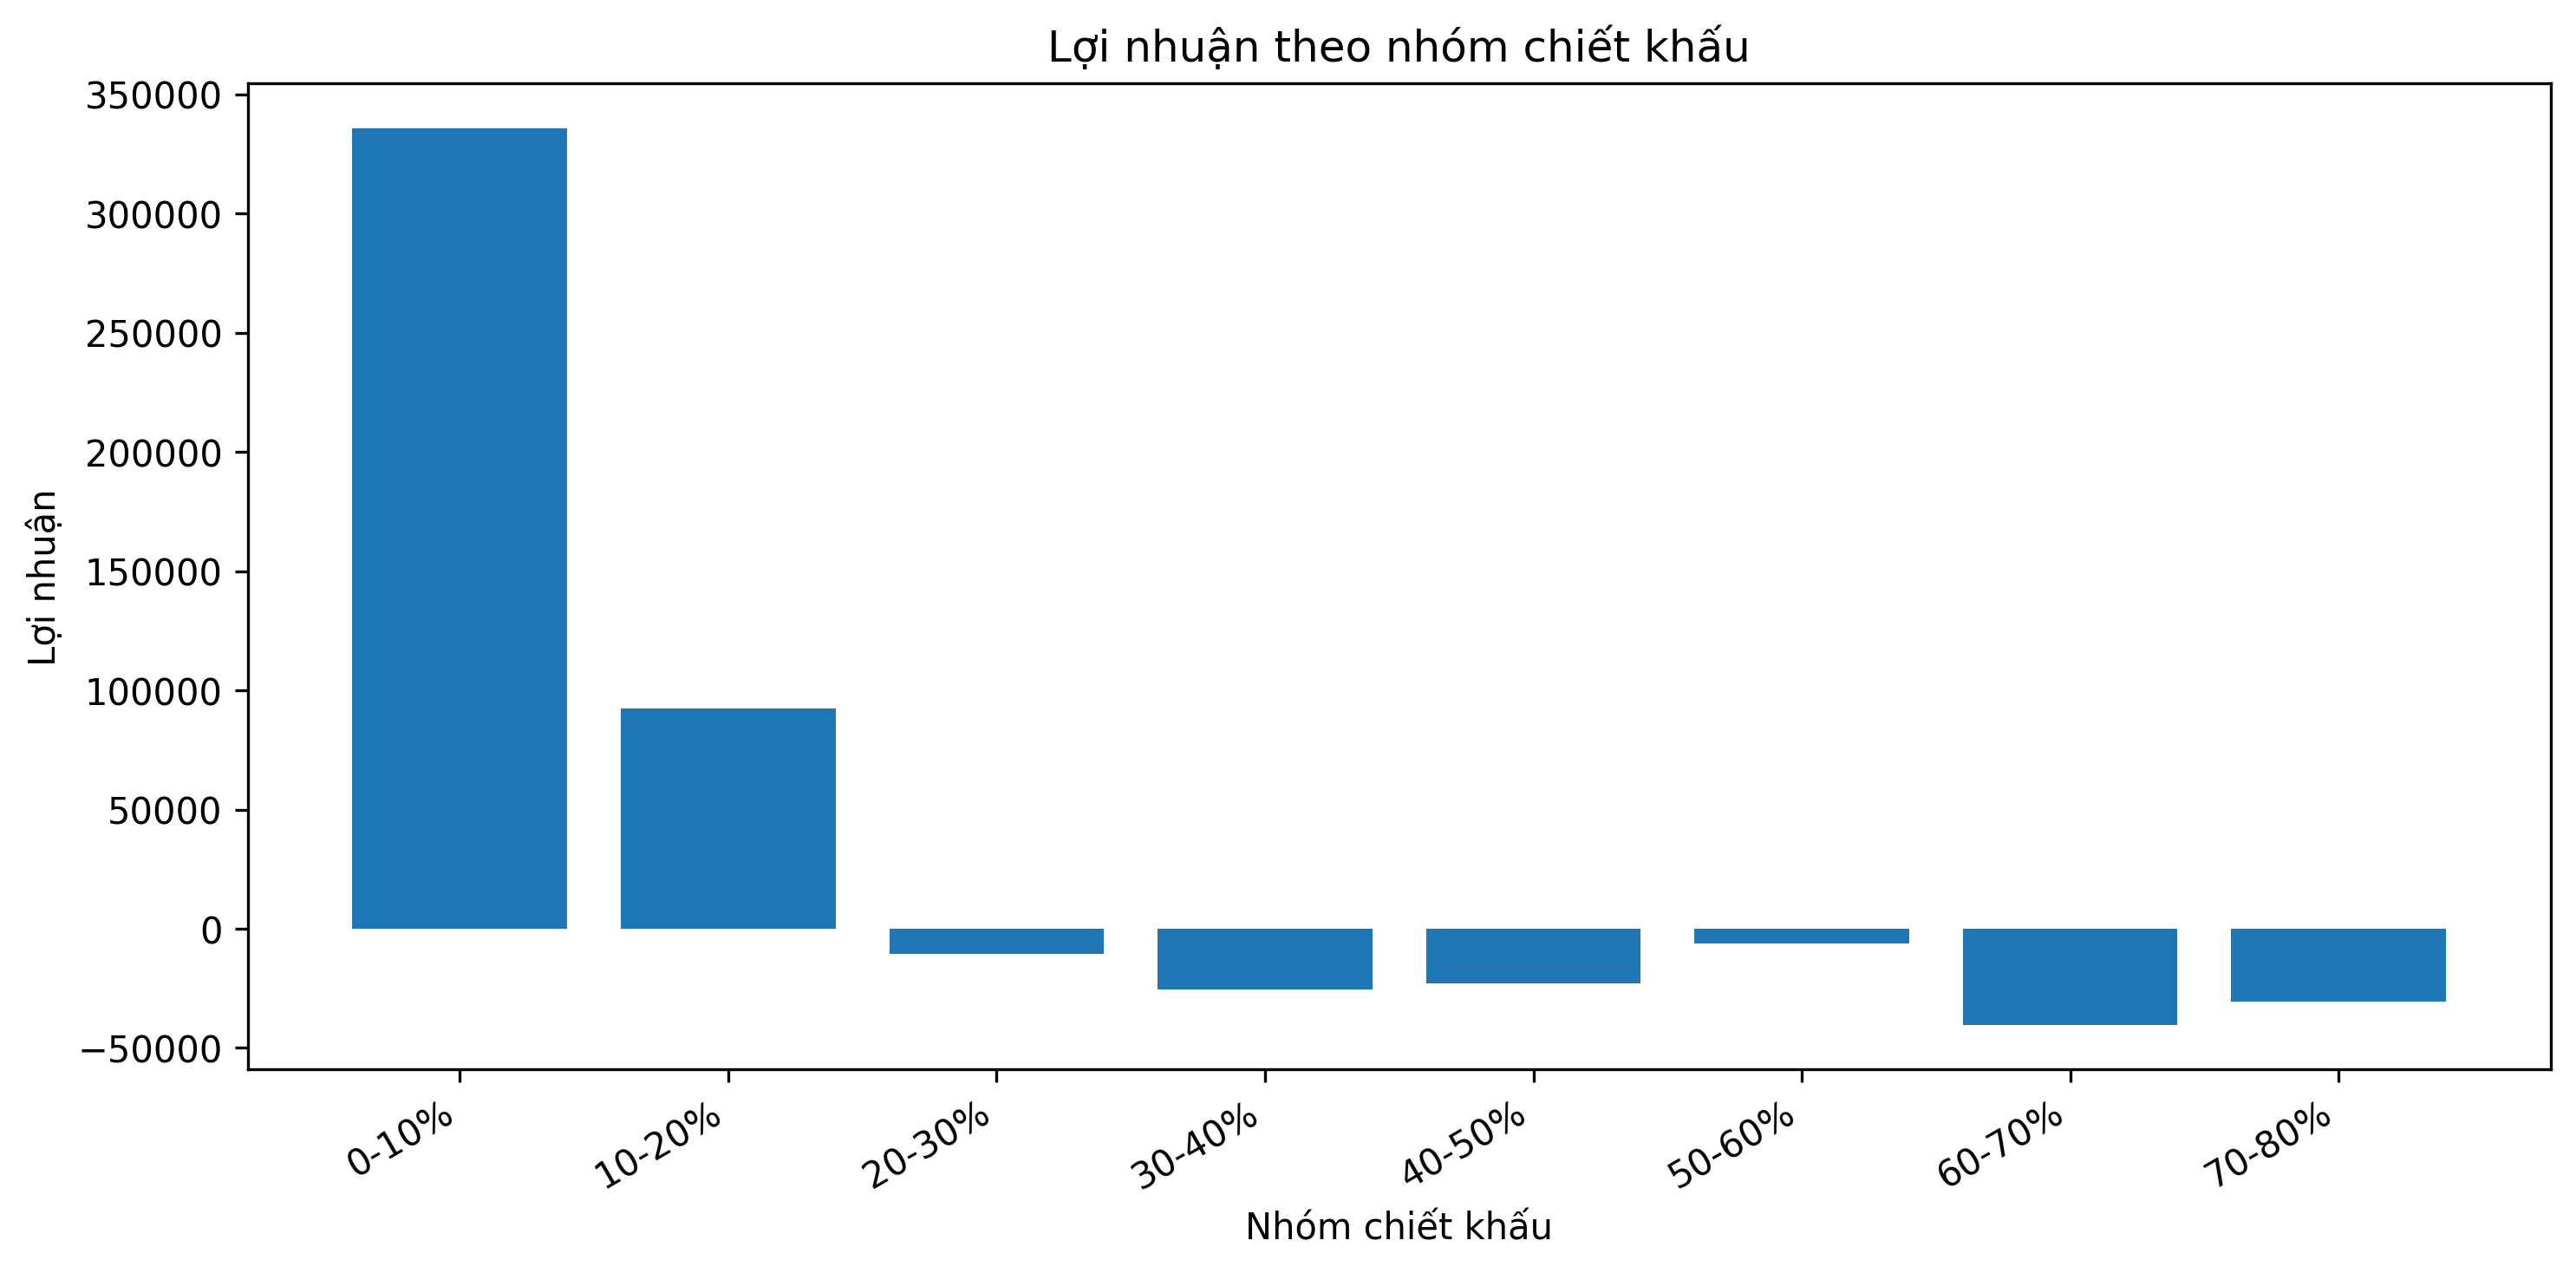
\includegraphics[width=0.9\textwidth]{images/anh_chuong3/hinh_3_6_loi_nhuan_theo_nhom_chiet_khau.png}
\caption{Lợi nhuận theo nhóm chiết khấu}
\label{fig:loi-nhuan-chiet-khau}
\end{figure}

Kết quả trên cho thấy chiết khấu cao có xu hướng làm giảm lợi nhuận, đặc biệt ở các nhóm từ 60--80\%. Đây là một insight quan trọng vì doanh nghiệp không chỉ cần quan tâm đến việc tăng doanh thu thông qua giảm giá mà còn phải kiểm soát tác động của chiết khấu đến hiệu quả sinh lời.

\section{Thiết kế và xây dựng dashboard trong Power BI}

\refstepcounter{subsection}
\subsection*{\thesubsection\quad Mục tiêu thiết kế dashboard}

Dashboard được xây dựng nhằm trực quan hóa các kết quả phân tích chính của bộ dữ liệu Superstore Sales, giúp tổng hợp các chỉ số quan trọng, biểu diễn dữ liệu dưới dạng biểu đồ và hỗ trợ người dùng theo dõi tình hình kinh doanh một cách trực quan. Trong đồ án này, dashboard được thiết kế với mục tiêu hỗ trợ trả lời các câu hỏi nghiên cứu liên quan đến xu hướng doanh số, hiệu quả theo khu vực, theo danh mục sản phẩm, hành vi tiêu dùng của phân khúc khách hàng và ảnh hưởng của chiết khấu đến lợi nhuận.

Các chỉ tiêu chính được sử dụng trên dashboard gồm tổng doanh thu, tổng lợi nhuận, số lượng bán, số đơn hàng, số khách hàng, doanh thu theo thời gian, doanh thu và lợi nhuận theo khu vực, lợi nhuận theo danh mục sản phẩm, doanh thu theo phân khúc khách hàng và lợi nhuận theo mức chiết khấu.

\refstepcounter{subsection}
\subsection*{\thesubsection\quad Cấu trúc dashboard}

Dashboard Power BI được tổ chức thành ba trang chính nhằm bảo đảm nội dung phân tích có tính hệ thống và dễ theo dõi:

\begin{itemize}
    \item \textbf{Trang 1: Tổng quan kinh doanh.} Trang này tập trung vào các chỉ số tổng quan như tổng doanh thu, tổng lợi nhuận, số lượng bán, số đơn hàng và xu hướng doanh thu theo thời gian.
    \item \textbf{Trang 2: Khu vực và sản phẩm.} Trang này phân tích doanh thu, lợi nhuận theo khu vực, danh mục và tiểu danh mục sản phẩm, từ đó hỗ trợ nhận diện khu vực và nhóm sản phẩm hoạt động hiệu quả.
    \item \textbf{Trang 3: Khách hàng và chiết khấu.} Trang này tập trung phân tích doanh thu theo phân khúc khách hàng và ảnh hưởng của chiết khấu đến lợi nhuận.
\end{itemize}

\begin{figure}[H]
\centering
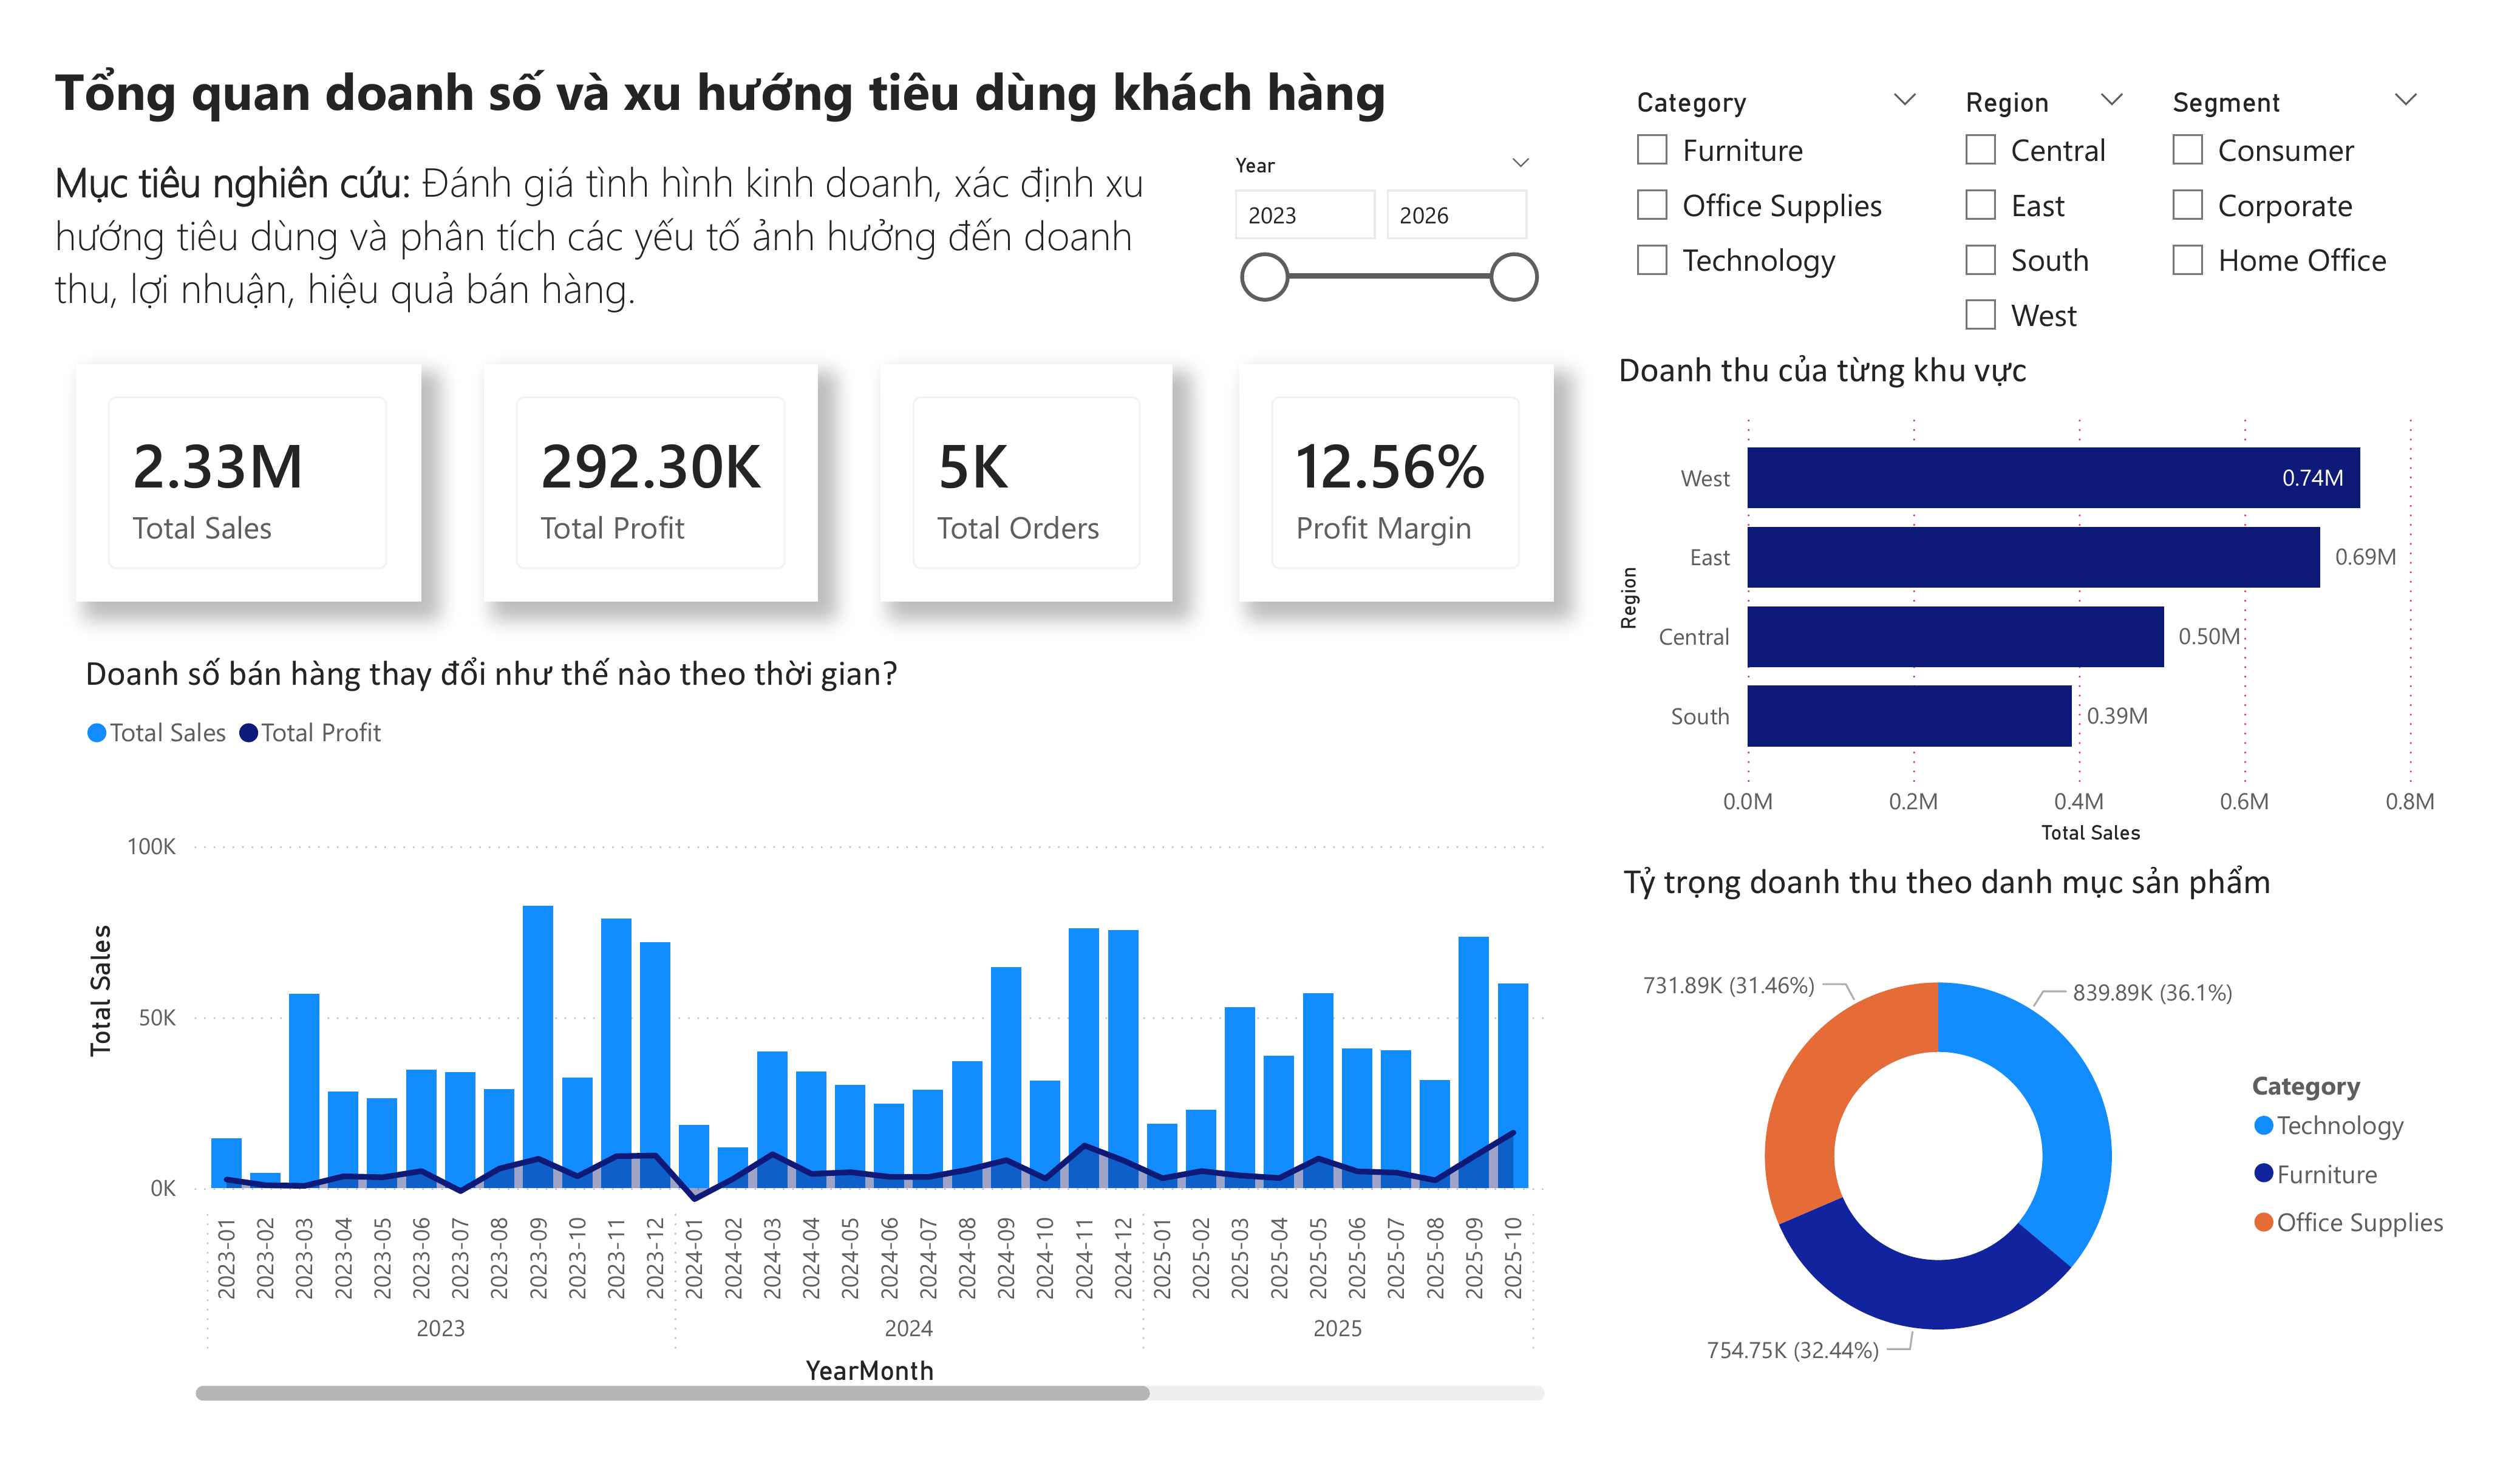
\includegraphics[width=0.95\textwidth]{images/anh_chuong3/dashboard_tong_quan_kinh_doanh.png}
\caption{Trang tổng quan kinh doanh trên Power BI}
\label{fig:dashboard-tong-quan}
\end{figure}

\begin{figure}[H]
\centering
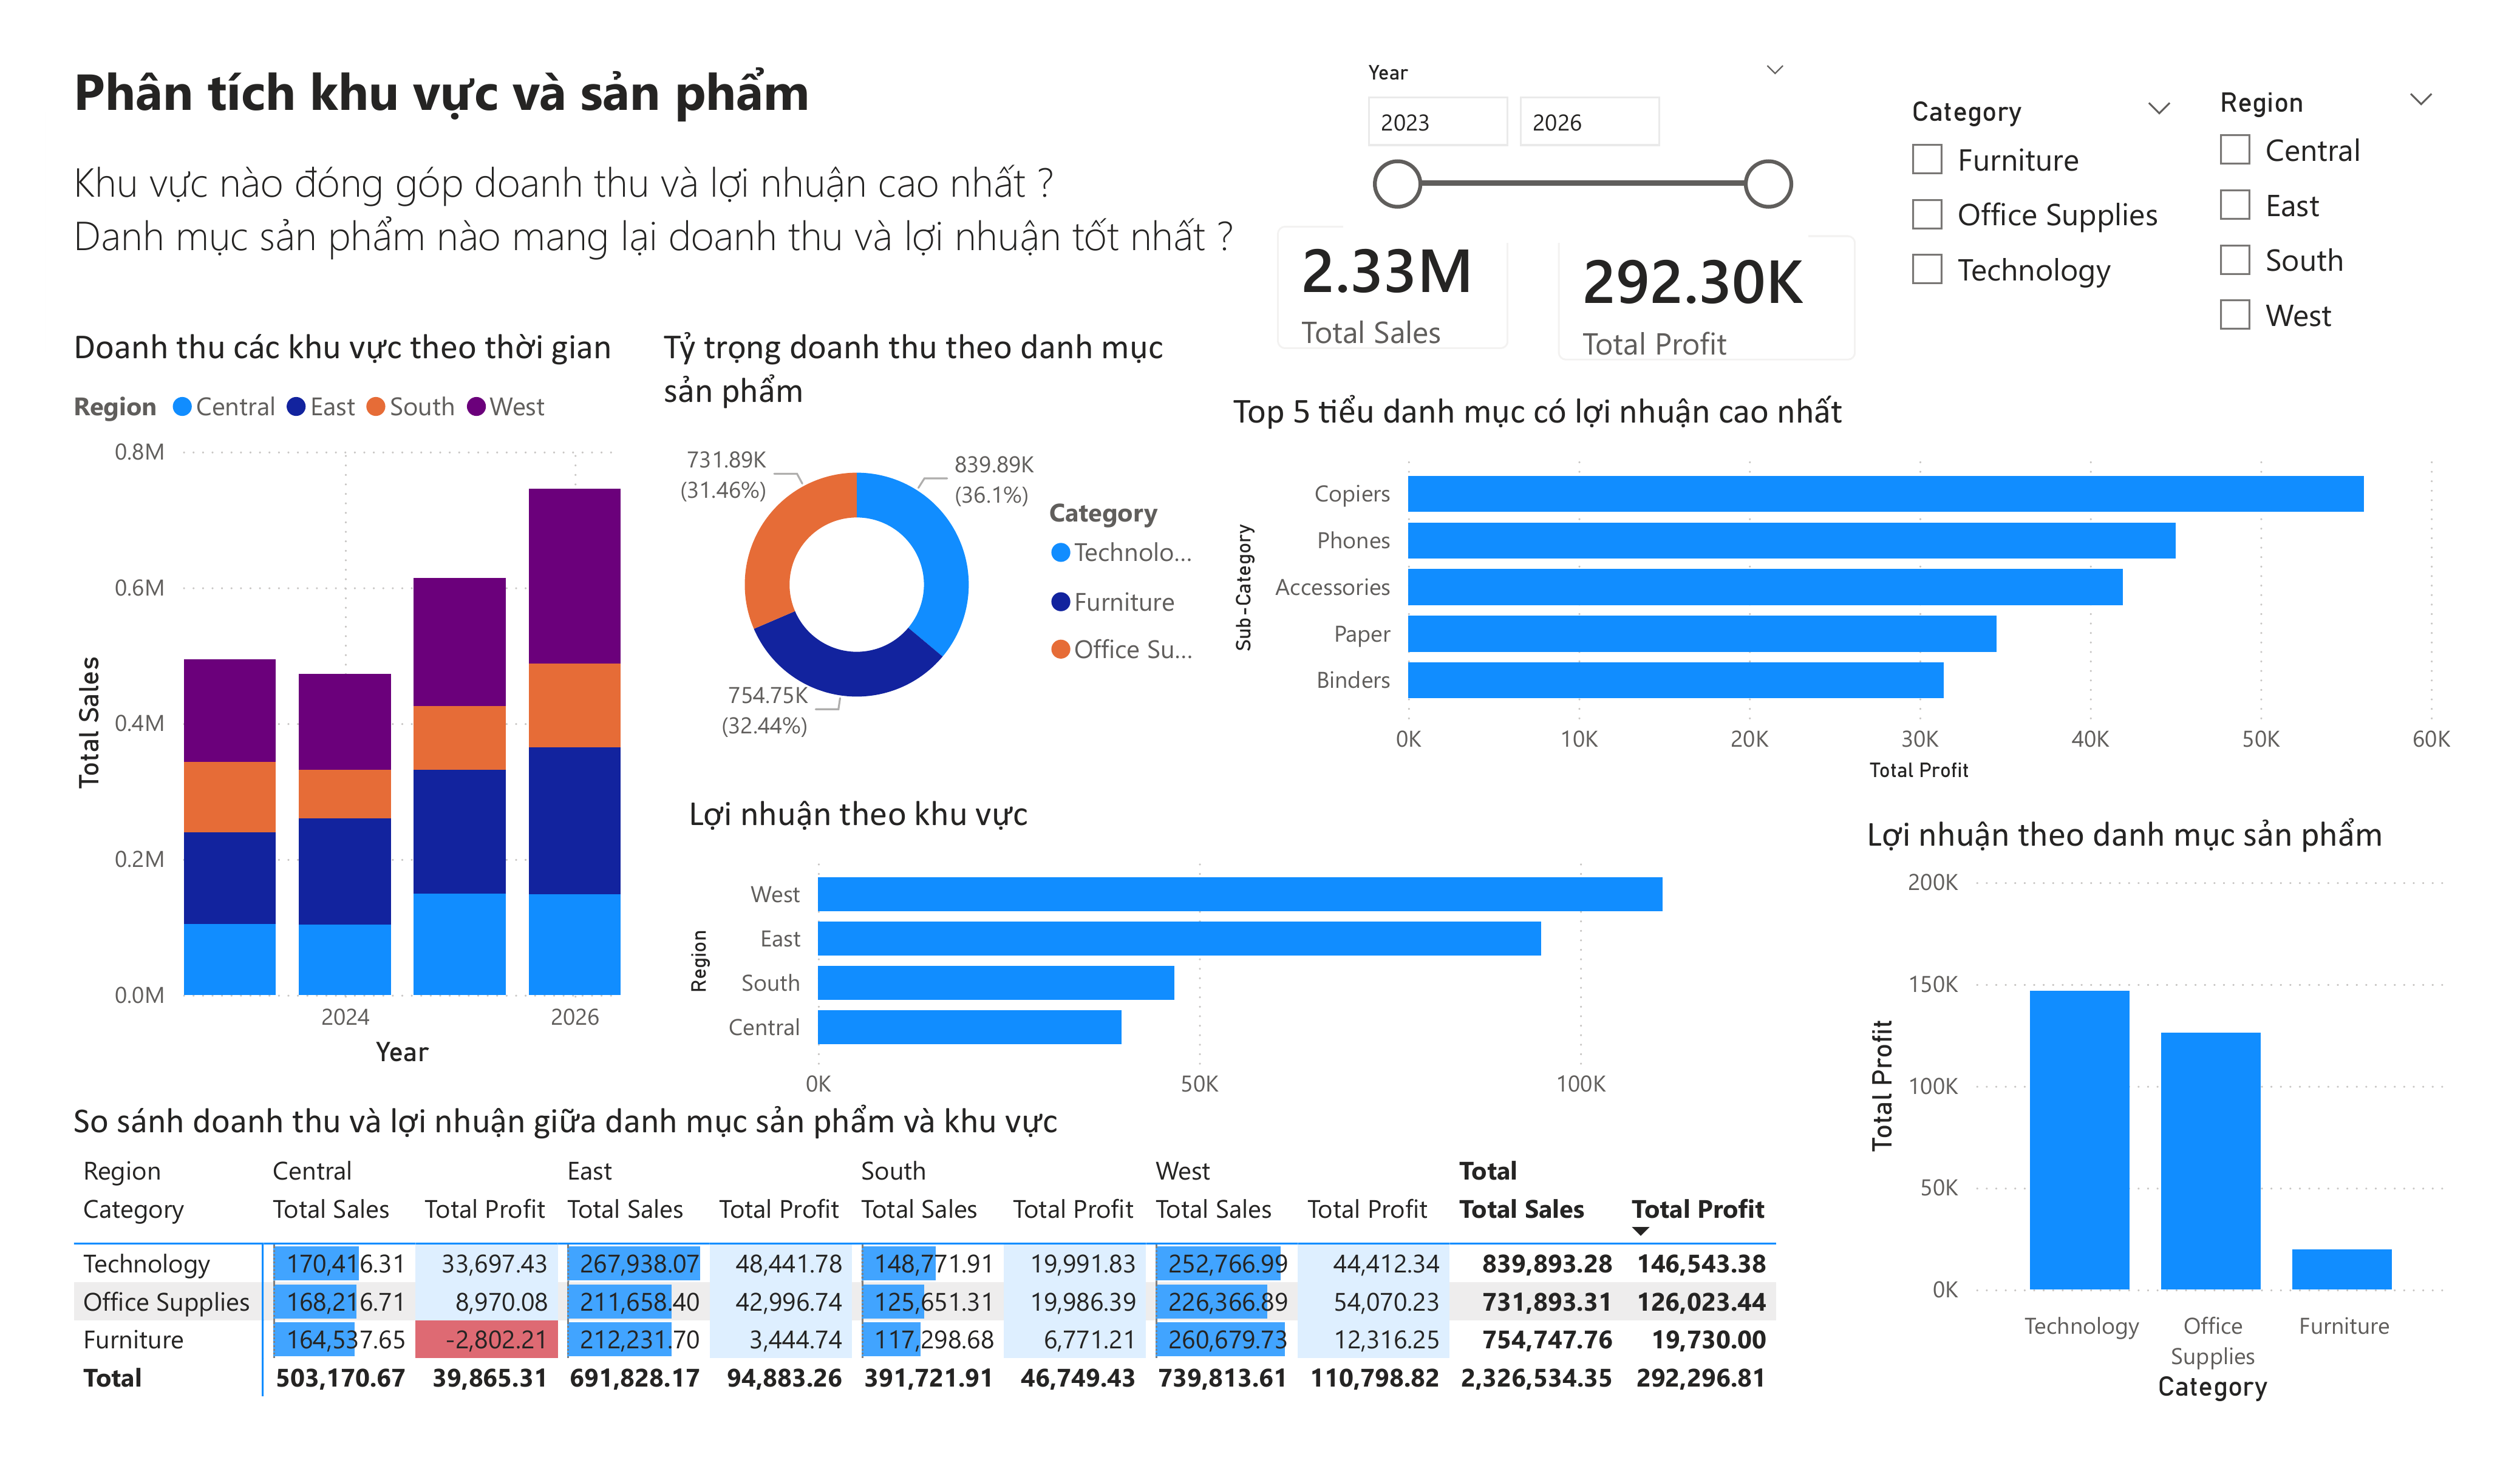
\includegraphics[width=0.95\textwidth]{images/anh_chuong3/dashboard_khu_vuc_san_pham.png}
\caption{Trang phân tích khu vực và sản phẩm trên Power BI}
\label{fig:dashboard-khu-vuc-san-pham}
\end{figure}

\begin{figure}[H]
\centering
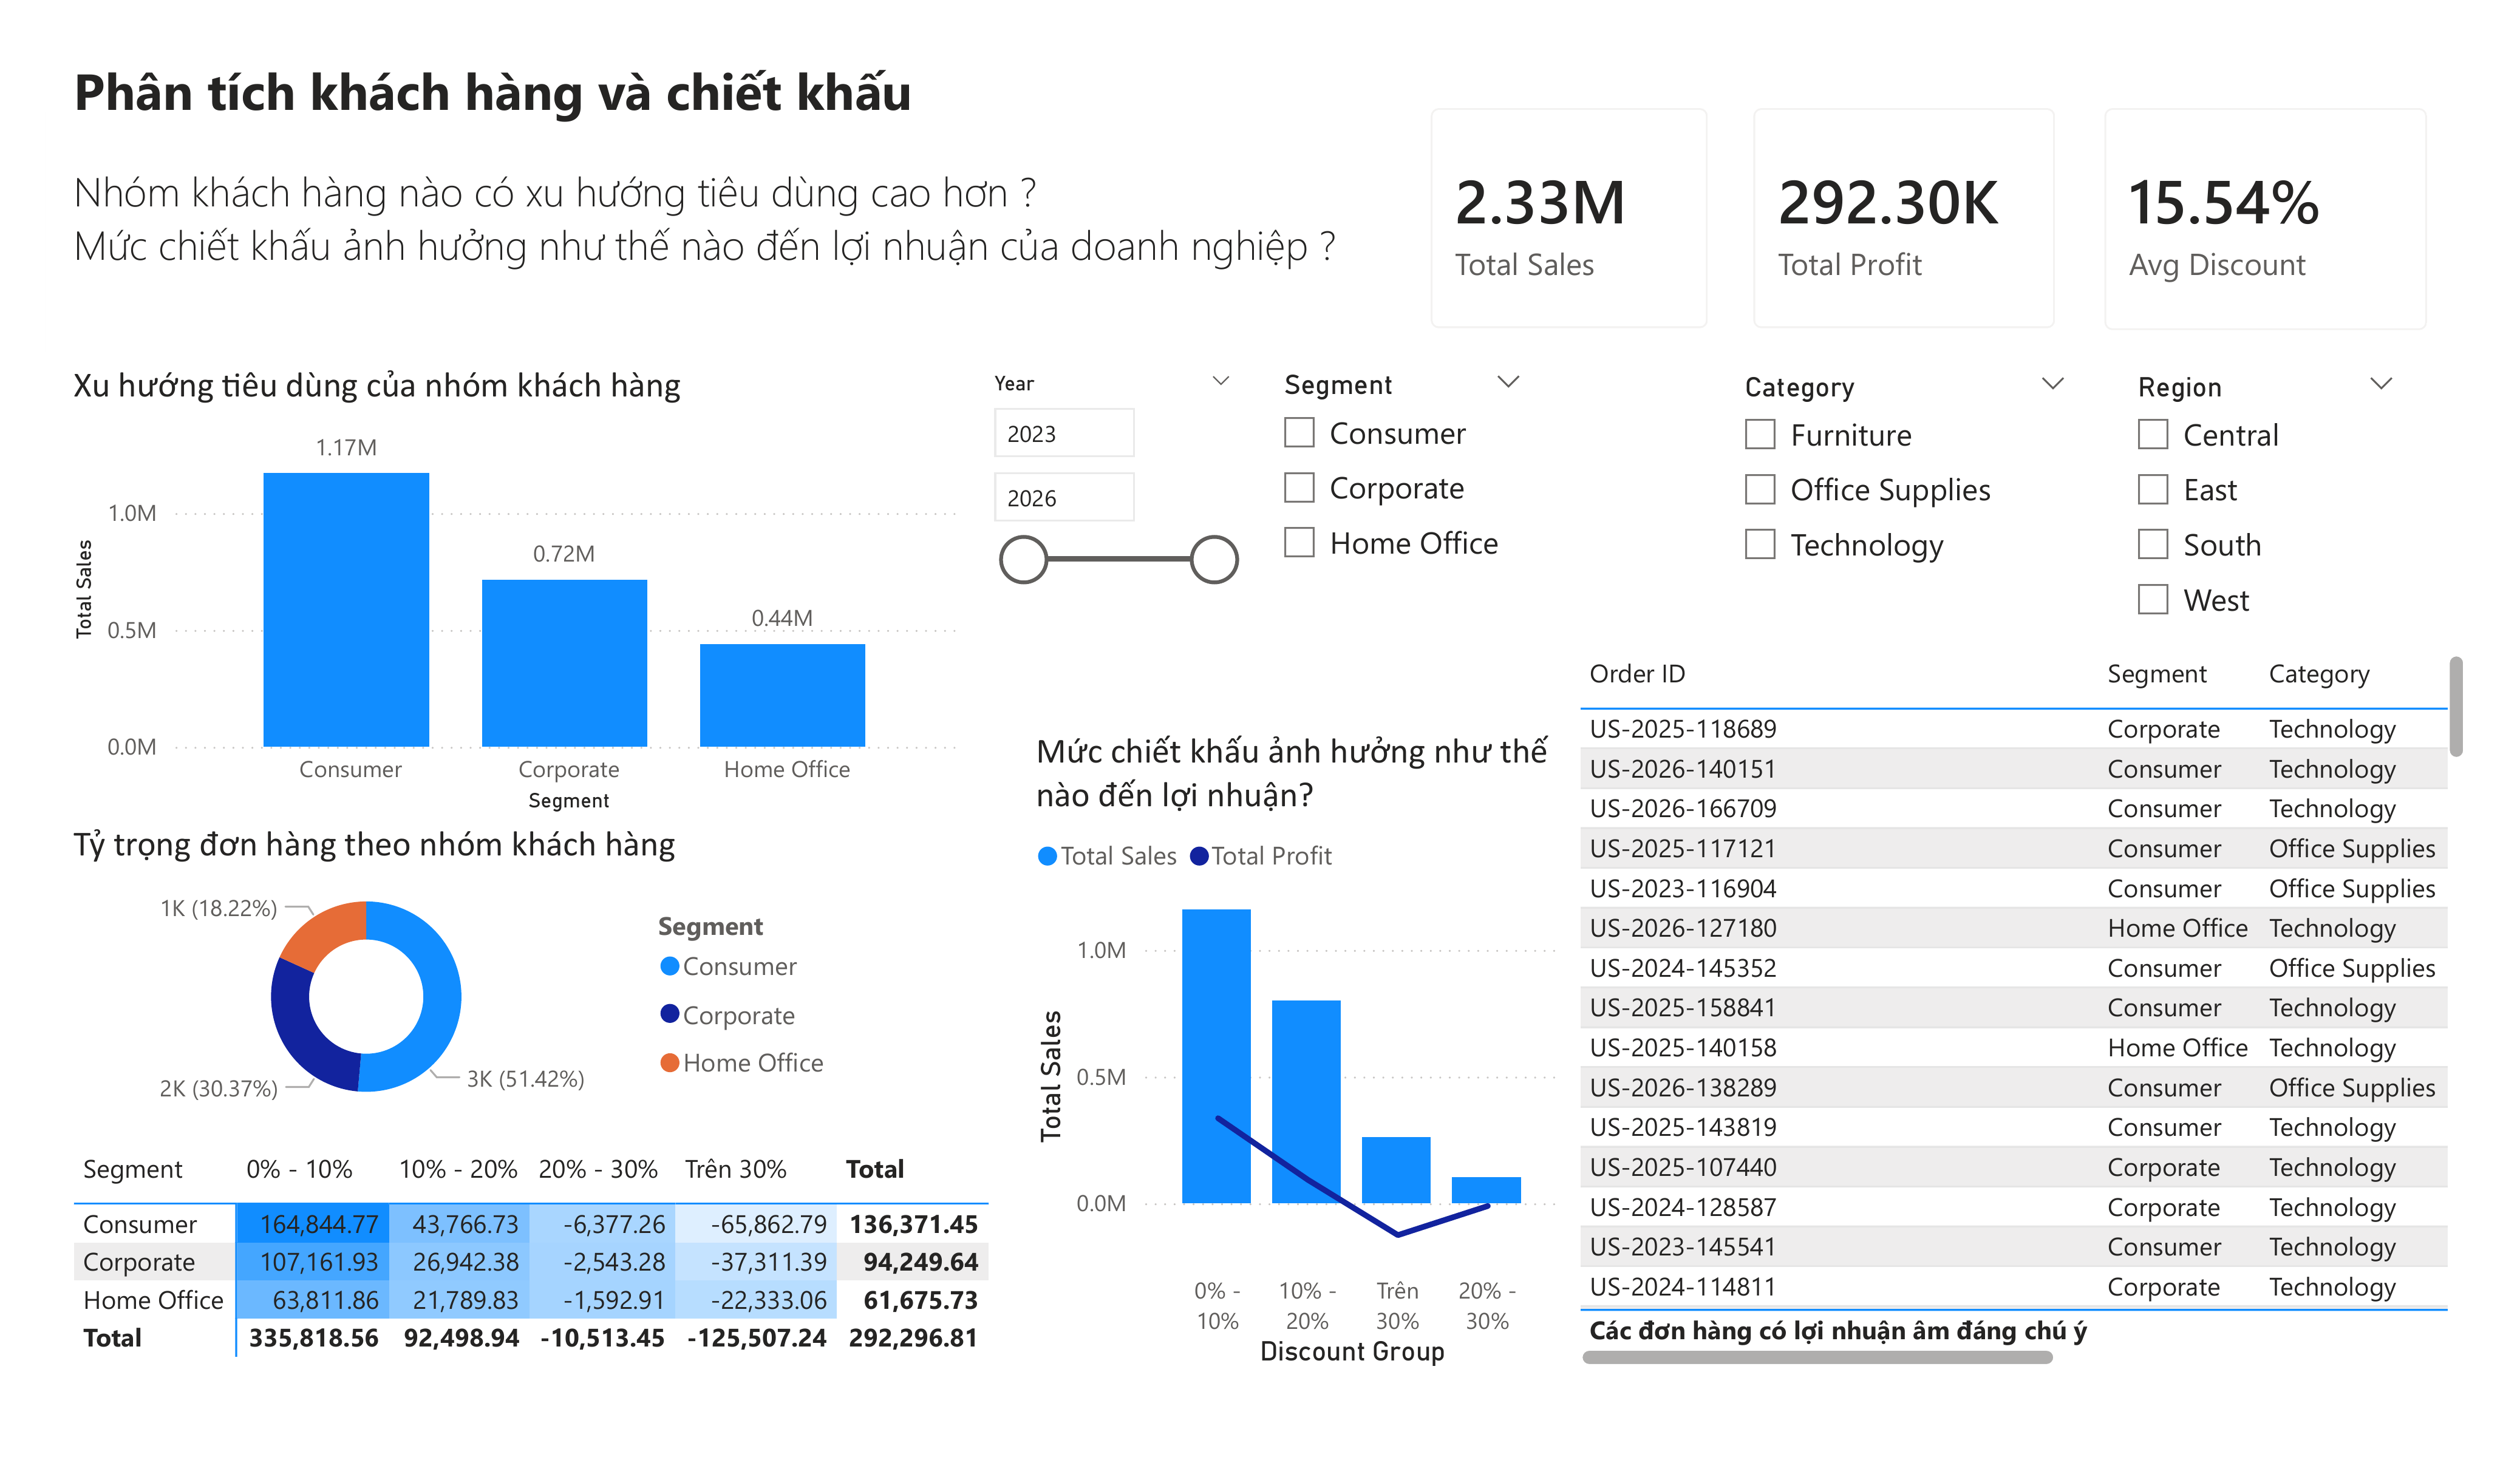
\includegraphics[width=0.95\textwidth]{images/anh_chuong3/dashboard_khach_hang_chiet_khau.png}
\caption{Trang phân tích khách hàng và chiết khấu trên Power BI}
\label{fig:dashboard-khach-hang-chiet-khau}
\end{figure}

\section{Diễn giải ý nghĩa biểu đồ và bộ lọc trên dashboard}

\refstepcounter{subsection}
\subsection*{\thesubsection\quad Nhóm biểu đồ tổng quan kinh doanh}

Nhóm biểu đồ tổng quan kinh doanh được sử dụng để cung cấp cái nhìn nhanh về tình hình hoạt động của doanh nghiệp. Các thẻ chỉ số như tổng doanh thu, tổng lợi nhuận, số lượng bán và số đơn hàng giúp người xem nắm bắt quy mô kinh doanh ở mức tổng quát. Biểu đồ doanh thu theo thời gian hỗ trợ nhận diện xu hướng tăng giảm của doanh số theo năm, quý hoặc tháng. Đây là nhóm biểu đồ trả lời trực tiếp câu hỏi nghiên cứu về sự thay đổi của doanh số bán hàng theo thời gian.

\refstepcounter{subsection}
\subsection*{\thesubsection\quad Nhóm biểu đồ phân tích khu vực và sản phẩm}

Nhóm biểu đồ khu vực và sản phẩm giúp so sánh hiệu quả kinh doanh giữa các vùng thị trường và các nhóm sản phẩm. Biểu đồ doanh thu theo khu vực cho biết khu vực nào đóng góp doanh thu lớn nhất. Biểu đồ lợi nhuận theo khu vực cho phép đánh giá khu vực nào hoạt động hiệu quả hơn về mặt sinh lời. Bên cạnh đó, biểu đồ lợi nhuận theo danh mục và tiểu danh mục sản phẩm giúp nhận diện nhóm sản phẩm có khả năng tạo lợi nhuận cao hoặc đang gây lỗ. Nhóm biểu đồ này hỗ trợ trả lời các câu hỏi nghiên cứu về khu vực và danh mục sản phẩm mang lại doanh thu, lợi nhuận tốt nhất.

\refstepcounter{subsection}
\subsection*{\thesubsection\quad Nhóm biểu đồ phân tích khách hàng và chiết khấu}

Nhóm biểu đồ khách hàng và chiết khấu tập trung vào hai khía cạnh: phân khúc khách hàng và chính sách giảm giá. Biểu đồ doanh thu theo phân khúc khách hàng giúp xác định nhóm khách hàng có mức tiêu dùng cao hơn. Trong khi đó, biểu đồ lợi nhuận theo nhóm chiết khấu cho thấy tác động của mức giảm giá đến hiệu quả kinh doanh. Nếu chiết khấu tăng nhưng lợi nhuận giảm mạnh, doanh nghiệp cần xem xét lại chính sách khuyến mại để tránh tăng doanh thu nhưng làm giảm hiệu quả sinh lời.

\refstepcounter{subsection}
\subsection*{\thesubsection\quad Ý nghĩa các bộ lọc tương tác}

Các bộ lọc trên dashboard giúp người dùng phân tích dữ liệu theo từng lát cắt cụ thể. Bộ lọc theo năm hỗ trợ so sánh kết quả kinh doanh giữa các giai đoạn. Bộ lọc theo khu vực giúp quan sát riêng từng vùng thị trường. Bộ lọc theo danh mục sản phẩm giúp phân tích sâu từng nhóm hàng. Bộ lọc theo phân khúc khách hàng giúp đánh giá hành vi tiêu dùng của từng nhóm đối tượng. Nhờ các bộ lọc này, dashboard không chỉ trình bày dữ liệu ở mức tổng quan mà còn hỗ trợ người dùng khai thác dữ liệu linh hoạt theo nhu cầu phân tích.

\begin{table}[H]
\centering
\caption{Ý nghĩa phân tích của các thành phần trên dashboard}
\label{tab:y-nghia-dashboard}
\begin{tabular}{p{4.5cm} p{8.5cm}}
\hline
\textbf{Thành phần dashboard} & \textbf{Ý nghĩa phân tích} \\
\hline
Thẻ tổng doanh thu & Cho biết quy mô doanh số của toàn bộ dữ liệu hoặc theo điều kiện lọc cụ thể. \\
\hline
Thẻ tổng lợi nhuận & Đánh giá hiệu quả sinh lời tổng thể của hoạt động bán hàng. \\
\hline
Biểu đồ doanh thu theo thời gian & Nhận diện xu hướng tăng giảm doanh số theo năm, quý hoặc tháng. \\
\hline
Biểu đồ doanh thu/lợi nhuận theo khu vực & So sánh mức đóng góp và hiệu quả kinh doanh giữa các khu vực. \\
\hline
Biểu đồ lợi nhuận theo danh mục sản phẩm & Xác định nhóm sản phẩm tạo lợi nhuận tốt hoặc có hiệu quả thấp. \\
\hline
Biểu đồ doanh thu theo phân khúc khách hàng & Nhận diện nhóm khách hàng có xu hướng tiêu dùng cao hơn. \\
\hline
Biểu đồ chiết khấu và lợi nhuận & Đánh giá tác động của chính sách giảm giá đến lợi nhuận. \\
\hline
Bộ lọc tương tác & Hỗ trợ phân tích dữ liệu theo từng năm, khu vực, sản phẩm hoặc phân khúc khách hàng. \\
\hline
\end{tabular}
\end{table}

\section{Đánh giá khả năng hỗ trợ phân tích của dashboard}

\refstepcounter{subsection}
\subsection*{\thesubsection\quad Khả năng hỗ trợ theo dõi và so sánh dữ liệu}

Dashboard giúp tổng hợp nhiều chỉ tiêu kinh doanh quan trọng trong cùng một giao diện, từ đó hỗ trợ người dùng quan sát nhanh tình hình doanh thu, lợi nhuận, sản phẩm, khu vực và khách hàng. So với việc xem dữ liệu dưới dạng bảng, dashboard giúp quá trình nhận diện xu hướng và so sánh giữa các nhóm trở nên trực quan hơn. Người dùng có thể nhanh chóng nhận ra khu vực nào có doanh thu cao, danh mục nào có lợi nhuận tốt, phân khúc khách hàng nào đóng góp nhiều và mức chiết khấu nào có nguy cơ làm giảm lợi nhuận.

\refstepcounter{subsection}
\subsection*{\thesubsection\quad Khả năng hỗ trợ trả lời câu hỏi nghiên cứu}

Dashboard có khả năng hỗ trợ trả lời các câu hỏi nghiên cứu đã đặt ra trong đề tài. Cụ thể, biểu đồ doanh thu theo thời gian giúp đánh giá sự thay đổi của doanh số qua các năm và tháng. Biểu đồ theo khu vực giúp xác định vùng thị trường có đóng góp cao nhất. Biểu đồ theo danh mục và tiểu danh mục sản phẩm giúp nhận diện nhóm hàng mang lại lợi nhuận tốt. Biểu đồ theo phân khúc khách hàng giúp xác định nhóm khách hàng có xu hướng tiêu dùng cao hơn. Cuối cùng, biểu đồ liên quan đến chiết khấu và lợi nhuận giúp đánh giá ảnh hưởng của chính sách giảm giá đến hiệu quả kinh doanh.

\refstepcounter{subsection}
\subsection*{\thesubsection\quad Hạn chế của dashboard và định hướng kết nối với mô hình phân tích}

Mặc dù dashboard có khả năng hỗ trợ tốt cho phân tích mô tả và so sánh trực quan, công cụ này vẫn có một số hạn chế. Dashboard chủ yếu giúp trả lời câu hỏi điều gì đã xảy ra và hỗ trợ nhận diện xu hướng trực quan, nhưng chưa đủ để đánh giá sâu mức độ ảnh hưởng của từng biến hoặc dự báo kết quả trong tương lai. Do đó, để nâng cao chiều sâu phân tích, các chương tiếp theo sẽ xây dựng các mô hình phân tích dữ liệu như hồi quy tuyến tính đa biến, Random Forest Regressor, Gradient Boosting Regressor, XGBoost Regressor và K-Means Clustering. Việc kết hợp dashboard với mô hình phân tích giúp đồ án không chỉ dừng lại ở trực quan hóa dữ liệu mà còn mở rộng sang phân tích quan hệ, dự báo và phân nhóm khách hàng.
	
	\chapter{Xây dựng các mô hình phân tích dữ liệu}
	\section{Mục tiêu xây dựng các mô hình}

Sau quá trình phân tích khám phá dữ liệu và trực quan hóa, em tiếp tục xây dựng các mô hình phân tích dữ liệu nhằm khai thác sâu hơn mối quan hệ giữa các biến trong bộ dữ liệu Superstore Sales, hướng đến việc xây dựng các mô hình thực nghiệm nhằm dự báo lợi nhuận và phân tích đặc điểm tiêu dùng của khách hàng.

Lợi nhuận là chỉ tiêu phản ánh trực tiếp hiệu quả kinh doanh, không chỉ thể hiện quy mô bán hàng mà còn cho biết mức độ sinh lời sau khi xét đến các yếu tố như chiết khấu, số lượng bán, nhóm sản phẩm và khu vực bán hàng. Do đó, việc dự báo lợi nhuận có ý nghĩa quan trọng trong việc hỗ trợ doanh nghiệp đánh giá hiệu quả hoạt động kinh doanh.

Mục tiêu chính của quá trình xây dựng mô hình gồm:
\begin{itemize}
    \item Dự báo lợi nhuận dựa trên các yếu tố đầu vào như số lượng bán, chiết khấu, phương thức giao hàng, khu vực, danh mục sản phẩm và phân khúc khách hàng.
    \item So sánh hiệu quả giữa các mô hình học máy khác nhau trên cùng bộ dữ liệu.
    \item Đánh giá ảnh hưởng của việc xử lý giá trị ngoại lai đến hiệu quả dự báo của từng mô hình.
    \item Nhận diện mô hình phù hợp hơn đối với bài toán dự báo lợi nhuận trong dữ liệu bán lẻ.
    \item Phân cụm khách hàng theo đặc điểm tiêu dùng nhằm hỗ trợ phân tích nhóm khách hàng.
\end{itemize}

Các mô hình được triển khai trong chương này gồm Hồi quy tuyến tính đa biến, Random Forest Regressor, Gradient Boosting Regressor, XGBoost Regressor và K-Means Clustering. Trong đó, bốn mô hình đầu tiên được sử dụng cho bài toán dự báo lợi nhuận, còn K-Means được sử dụng cho bài toán phân cụm khách hàng.

Quy trình xây dựng mô hình được thực hiện qua các bước chính: xác định mục tiêu phân tích, thu thập dữ liệu, làm sạch dữ liệu, xây dựng mô hình, thực hiện đánh giá mô hình, cải tiến mô hình, triển khai vào thực tế, theo dõi hiệu quả thực hiện.

\begin{figure}[H]
    \centering
    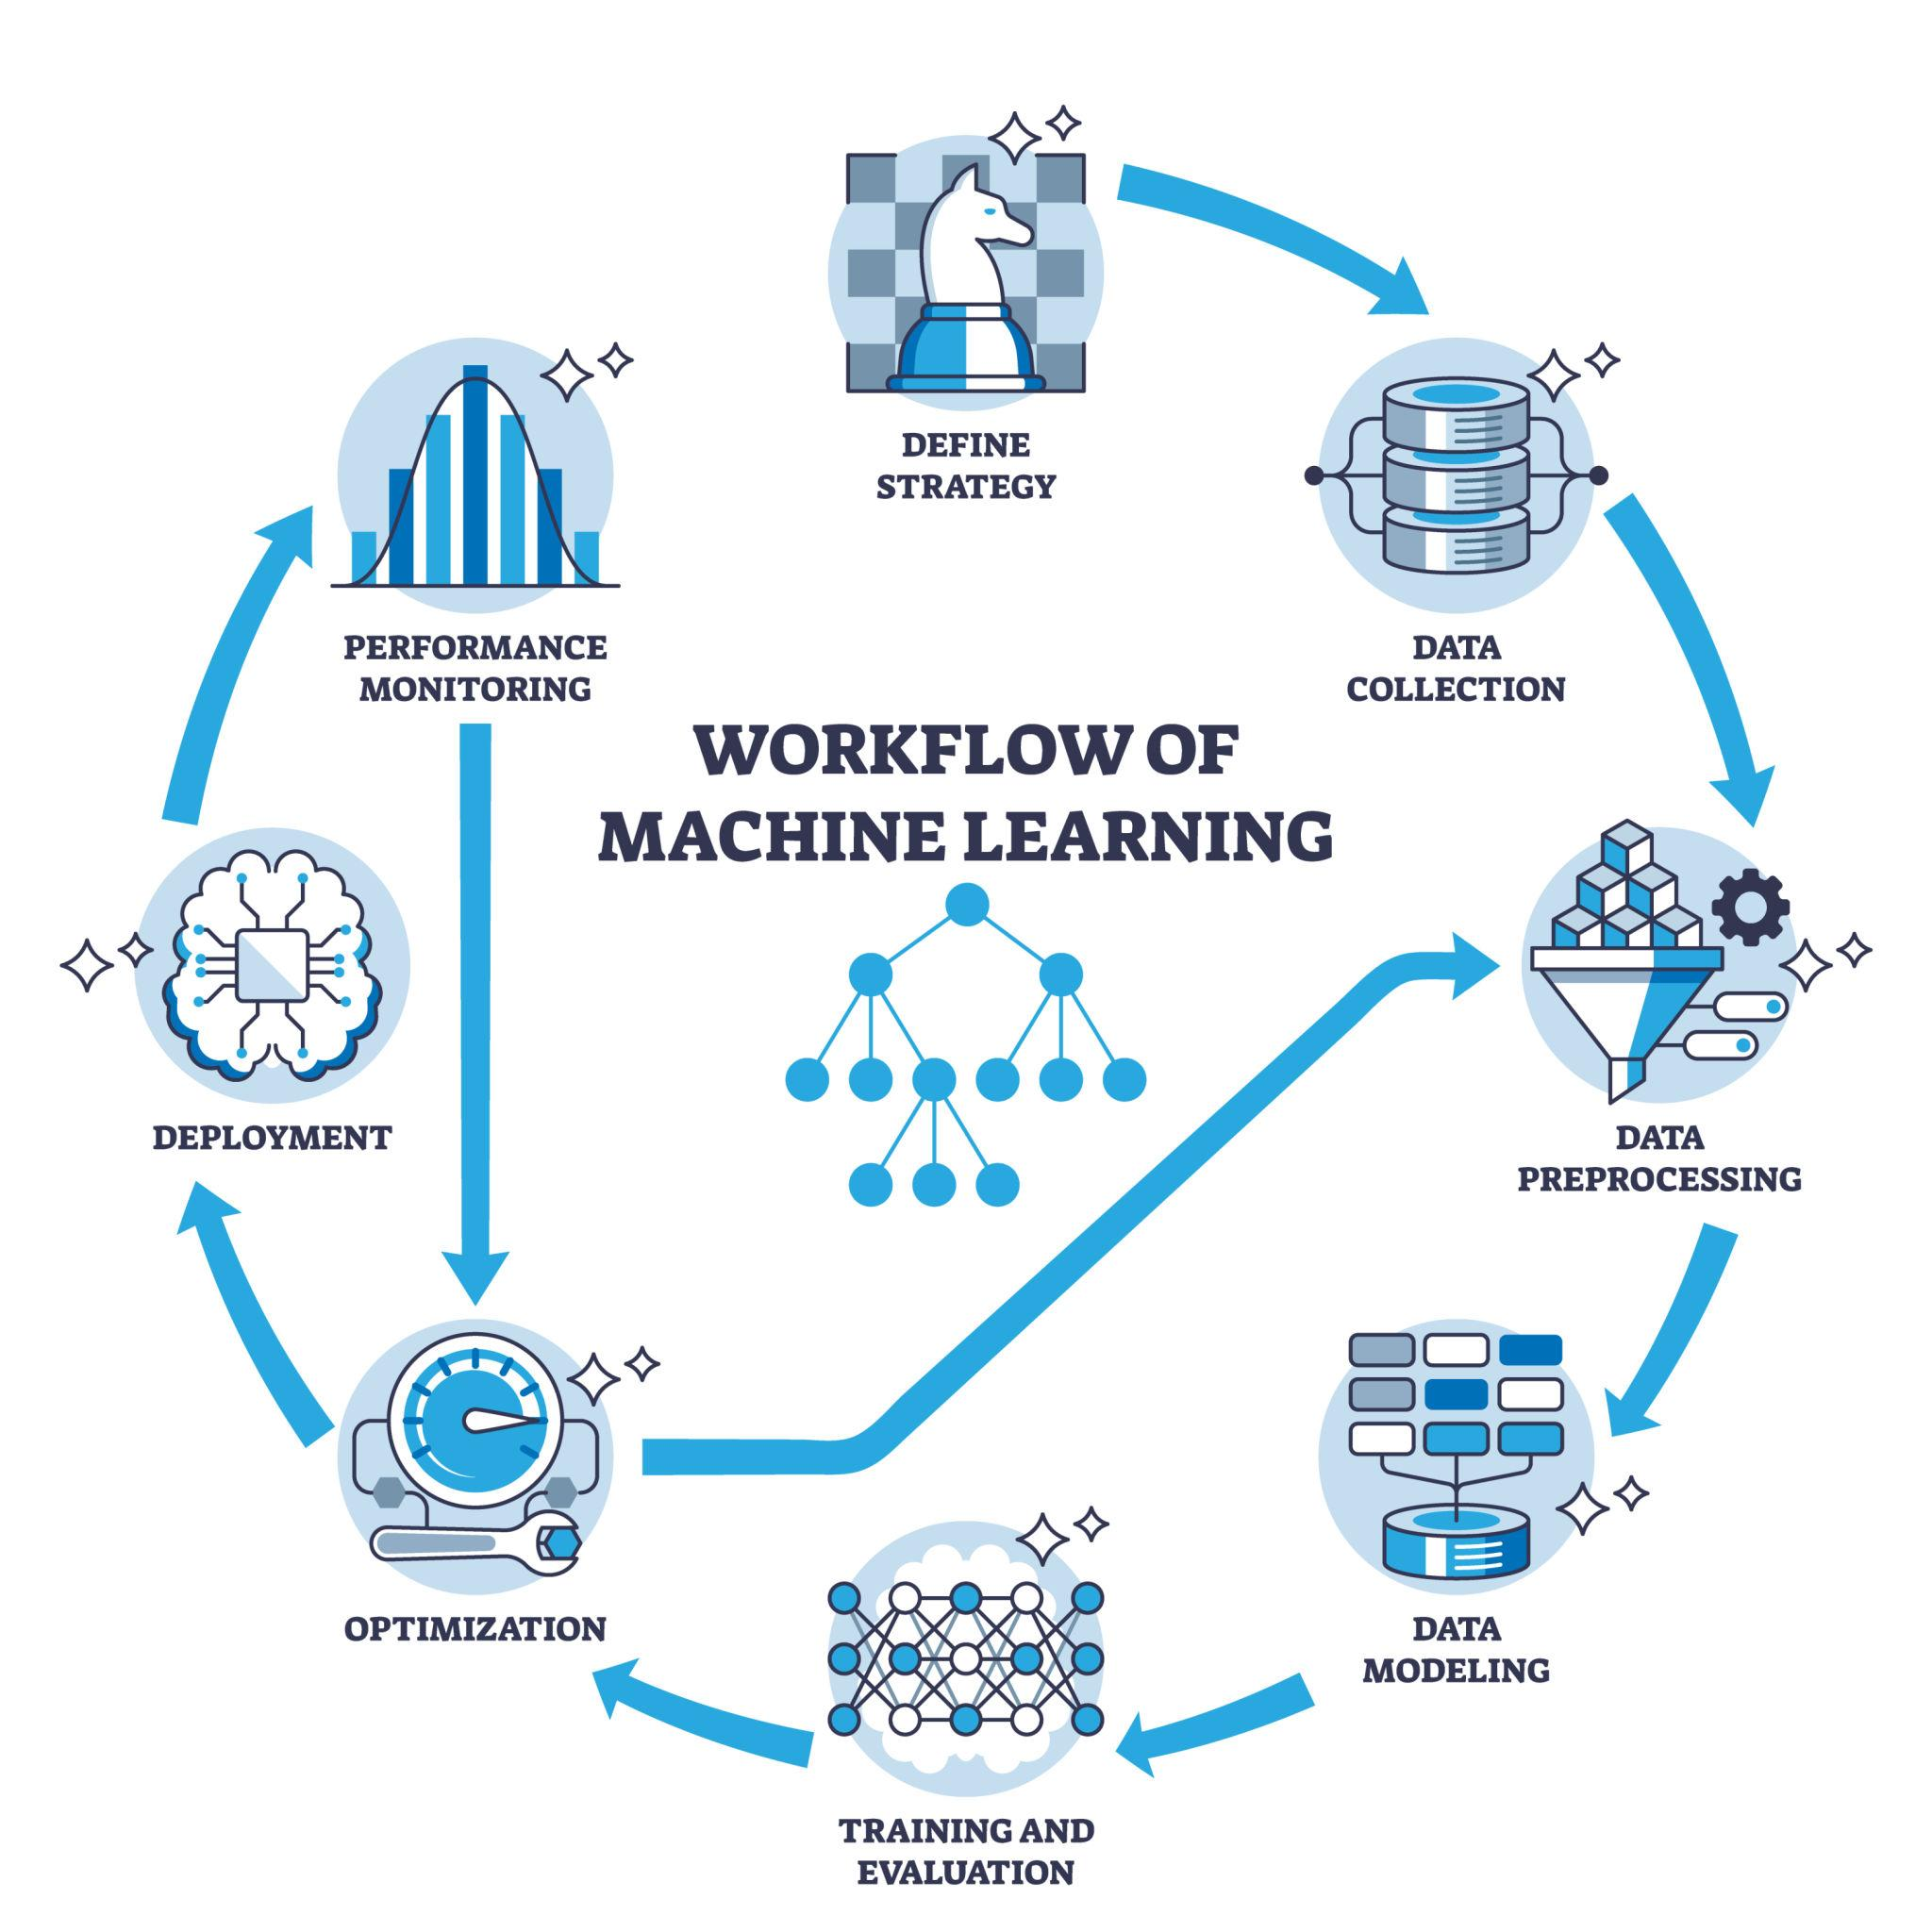
\includegraphics[width=0.85\textwidth]{images/anh_chuong4/model_workflow.png}
    \caption{Quy trình xây dựng và đánh giá mô hình phân tích dữ liệu}
    \label{fig:model_workflow}
\end{figure}

\section{Lựa chọn các biến phân tích}

Trong bài toán dự báo, biến mục tiêu được lựa chọn là \textbf{Profit}. Đây là biến phản ánh lợi nhuận thu được từ từng giao dịch và là chỉ tiêu quan trọng để đánh giá hiệu quả kinh doanh. Việc lựa chọn Profit làm biến mục tiêu giúp mô hình tập trung vào bài toán sinh lời thay vì chỉ dự báo quy mô doanh thu.

Các biến đầu vào được lựa chọn dựa trên đặc điểm của bộ dữ liệu và mục tiêu nghiên cứu, bao gồm:
\begin{itemize}
    \item \textbf{Quantity}: số lượng sản phẩm được bán trong mỗi giao dịch.
    \item \textbf{Discount}: mức chiết khấu được áp dụng.
    \item \textbf{Shipping Days}: số ngày giao hàng, được tính từ thời điểm đặt hàng đến thời điểm giao hàng.
    \item \textbf{Sales}: doanh thu của từng giao dịch.
    \item \textbf{Ship Mode}: phương thức giao hàng.
    \item \textbf{Segment}: phân khúc khách hàng.
    \item \textbf{Region}: khu vực bán hàng.
    \item \textbf{Category}: danh mục sản phẩm.
    \item \textbf{Sub-Category}: tiểu danh mục sản phẩm.
    \item \textbf{Year, Month, Quarter}: các biến thời gian được trích xuất từ ngày đặt hàng.
\end{itemize}

Một số biến định danh như \textit{Order ID}, \textit{Customer ID}, \textit{Customer Name}, \textit{Product ID} và \textit{Product Name} được loại bỏ khỏi tập dữ liệu đầu vào. Các biến này chủ yếu dùng để nhận diện đơn hàng, khách hàng hoặc sản phẩm cụ thể, không phản ánh trực tiếp quy luật dự báo lợi nhuận.

Đối với các biến định tính, đề tài sử dụng phương pháp One-Hot Encoding để chuyển đổi sang dạng số. Đây là bước cần thiết vì các mô hình học máy yêu cầu dữ liệu đầu vào ở dạng số. Đối với các biến số, dữ liệu được kiểm tra và xử lý ngoại lai bằng phương pháp IQR Capping trong trường hợp cần so sánh trước và sau xử lý ngoại lai.

Dữ liệu được chia thành hai phần:
\begin{itemize}
    \item Tập huấn luyện chiếm 80\% dữ liệu.
    \item Tập kiểm tra chiếm 20\% dữ liệu.
\end{itemize}

Việc chia dữ liệu thành tập huấn luyện và tập kiểm tra giúp đánh giá khả năng tổng quát hóa của mô hình. Nếu mô hình chỉ cho kết quả tốt trên tập huấn luyện nhưng kém trên tập kiểm tra, điều đó cho thấy mô hình có thể đang bị quá khớp với dữ liệu huấn luyện.

\begin{table}[H]
\centering
\caption{Các nhóm biến sử dụng trong quá trình xây dựng mô hình}
\label{tab:model_variables}
\begin{tabular}{|p{4cm}|p{8cm}|}
\hline
\textbf{Nhóm biến} & \textbf{Biến sử dụng} \\ \hline
Biến mục tiêu & Profit \\ \hline
Biến định lượng & Quantity, Discount, Shipping Days, Sales, Year, Month, Quarter \\ \hline
Biến định tính & Ship Mode, Segment, Region, Category, Sub-Category \\ \hline
Biến loại bỏ & Order ID, Customer ID, Customer Name, Product ID, Product Name \\ \hline
\end{tabular}
\end{table}

\section{Mô hình hồi quy tuyến tính đa biến}


\refstepcounter{subsection}
\subsection*{\thesubsection\quad Giới thiệu mô hình}


Hồi quy tuyến tính đa biến là mô hình cơ bản được sử dụng để mô tả mối quan hệ tuyến tính giữa nhiều biến độc lập và một biến phụ thuộc. Mô hình được sử dụng để dự báo lợi nhuận dựa trên các yếu tố như số lượng bán, chiết khấu, khu vực, phân khúc khách hàng, danh mục sản phẩm và thời gian giao hàng.

Mô hình hồi quy tuyến tính đa biến được lựa chọn làm mô hình cơ sở. Vai trò của mô hình này không chỉ là dự báo lợi nhuận mà còn giúp tạo ra một mốc so sánh ban đầu để đánh giá hiệu quả của các mô hình phức tạp hơn như Random Forest, Gradient Boosting và XGBoost.

Ưu điểm của mô hình hồi quy tuyến tính là dễ xây dựng, dễ diễn giải và phù hợp khi mối quan hệ giữa biến đầu vào và biến mục tiêu có xu hướng tuyến tính. Tuy nhiên, trong dữ liệu kinh doanh bán lẻ, mối quan hệ giữa các biến thường phức tạp hơn. Ví dụ, chiết khấu có thể giúp tăng doanh thu nhưng đồng thời làm giảm lợi nhuận. Vì vậy, mô hình hồi quy tuyến tính có thể gặp hạn chế khi áp dụng vào bài toán này.

\refstepcounter{subsection}
\subsection*{\thesubsection\quad Kết quả trước xử lý ngoại lai}

Trước khi xử lý giá trị ngoại lai, mô hình hồi quy tuyến tính đa biến cho kết quả thấp trên cả tập huấn luyện và tập kiểm tra. 

Cụ thể:
\begin{itemize}
	\item Tập huấn luyện đạt \(MAE = 74.2328\), \(RMSE = 223.1231\) và \(R^2 = 0.199\).
	\item Tập kiểm tra đạt \(MAE = 73.6679\), \(RMSE = 144.649\) và \(R^2 = 0.0305\).
\end{itemize}

Giá trị \(R^2\) trên tập kiểm tra rất thấp cho thấy mô hình gần như chưa giải thích được sự biến động của lợi nhuận trong dữ liệu kiểm tra. Điều này phản ánh khả năng dự báo của mô hình còn hạn chế khi dữ liệu vẫn tồn tại nhiều điểm ngoại lai.

\begin{figure}[H]
	\centering
	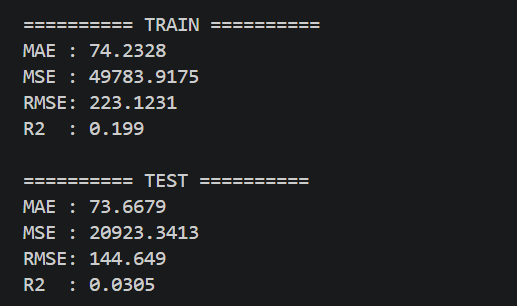
\includegraphics[width=0.6\textwidth]{images/anh_chuong4/linear_before_metrics.png}
	\caption{Kết quả mô hình hồi quy tuyến tính trước xử lý ngoại lai}
	\label{fig:linear_before_metrics}
\end{figure}

Nguyên nhân chủ yếu đến từ đặc điểm của dữ liệu bán lẻ. Bộ dữ liệu Superstore Sales có sự chênh lệch lớn giữa các giao dịch. Phần lớn các giao dịch có doanh thu và lợi nhuận ở mức trung bình hoặc thấp, trong khi một số giao dịch có lợi nhuận âm rất lớn hoặc lợi nhuận dương bất thường.


\begin{figure}[H]
	\centering
	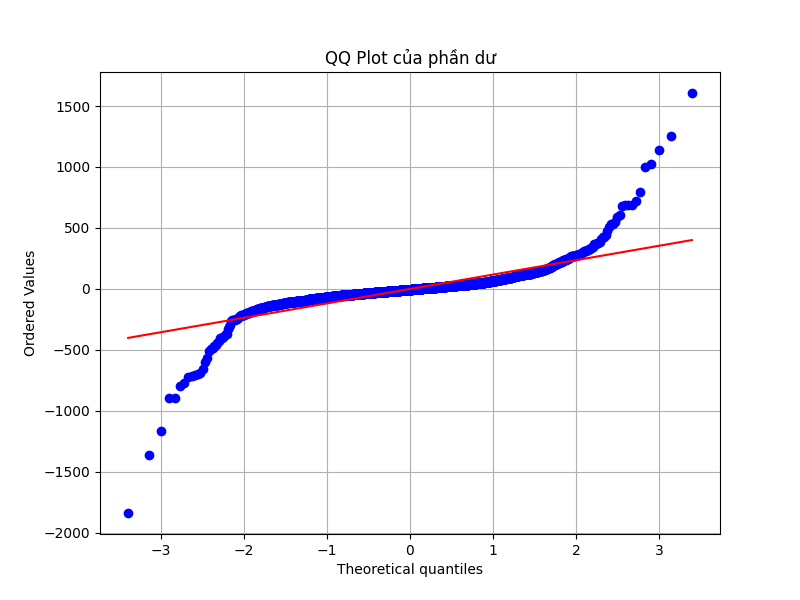
\includegraphics[width=0.75\textwidth]{images/anh_chuong4/linear_before_qqplot.png}
	\caption{QQ Plot phần dư trước xử lý ngoại lai}
	\label{fig:linear_before_qqplot}
\end{figure}

Quan sát QQ Plot trong Hình \ref{fig:linear_before_qqplot} cho thấy các điểm dữ liệu lệch khá xa khỏi đường thẳng chuẩn ở hai đầu phân phối. Điều này chứng tỏ phần dư của mô hình chưa tuân theo phân phối chuẩn và vẫn chịu ảnh hưởng mạnh của các giá trị ngoại lai.


\refstepcounter{subsection}
\subsection*{\thesubsection\quad Kết quả sau khi xử lý ngoại lai}

Sau khi áp dụng phương pháp IQR Capping để xử lý giá trị ngoại lai, hiệu quả của mô hình hồi quy tuyến tính đa biến được cải thiện rõ rệt trên cả tập huấn luyện và tập kiểm tra.

Cụ thể:
\begin{itemize}
	\item Tập huấn luyện đạt \(MAE = 16.8002\), \(RMSE = 21.3793\) và \(R^2 = 0.4707\).
	\item Tập kiểm tra đạt \(MAE = 18.4952\), \(RMSE = 23.4194\) và \(R^2 = 0.3617\).
\end{itemize}

So với trước khi xử lý ngoại lai, giá trị \(R^2\) trên tập kiểm tra đã tăng mạnh từ 0.0305 lên 0.3617. Đồng thời, các chỉ số MAE và RMSE giảm đáng kể. Điều này cho thấy việc xử lý ngoại lai giúp mô hình học tốt hơn xu hướng chung của dữ liệu và cải thiện đáng kể khả năng dự báo lợi nhuận.

\begin{figure}[H]
	\centering
	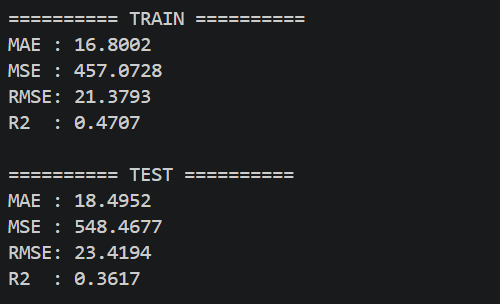
\includegraphics[width=0.6\textwidth]{images/anh_chuong4/linear_after_metrics.png}
	\caption{Kết quả mô hình hồi quy tuyến tính sau xử lý ngoại lai}
	\label{fig:linear_after_metrics}
\end{figure}

Nguyên nhân của sự cải thiện này là do các giá trị lợi nhuận quá lớn hoặc quá nhỏ đã được giới hạn trong khoảng hợp lý hơn. Việc giảm ảnh hưởng của các giao dịch bất thường giúp dữ liệu ổn định hơn và làm cho đường hồi quy phản ánh chính xác hơn xu hướng của phần lớn dữ liệu.



\begin{figure}[H]
	\centering
	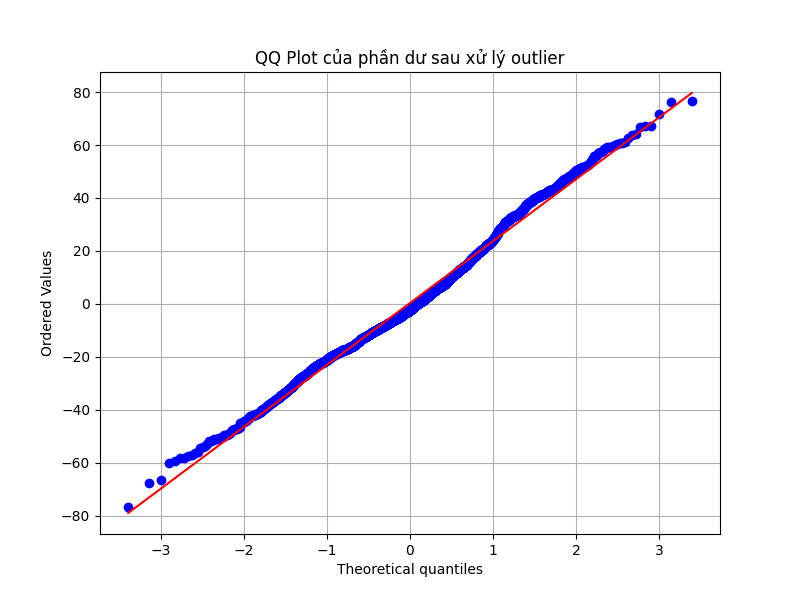
\includegraphics[width=0.75\textwidth]{images/anh_chuong4/linear_after_qqplot.png}
	\caption{QQ Plot phần dư sau xử lý ngoại lai}
	\label{fig:linear_after_qqplot}
\end{figure}

Quan sát QQ Plot trong Hình \ref{fig:linear_after_qqplot} cho thấy các điểm dữ liệu bám sát đường chuẩn hơn đáng kể so với trước khi xử lý ngoại lai. Điều này chứng tỏ phần dư của mô hình đã gần với phân phối chuẩn hơn.

Mặc dù ở hai đầu phân phối vẫn còn một số điểm lệch khỏi đường chuẩn, tuy nhiên mức độ lệch đã giảm rõ rệt. Điều này cho thấy việc xử lý ngoại lai đã giúp mô hình hồi quy tuyến tính hoạt động ổn định hơn và nâng cao khả năng dự báo trên bộ dữ liệu bán lẻ.

\refstepcounter{subsection}
\subsection*{\thesubsection\quad So sánh trước và sau xử lý ngoại lai}

Kết quả thực nghiệm cho thấy việc xử lý ngoại lai giúp cải thiện đáng kể hiệu quả của mô hình hồi quy tuyến tính đa biến. Sau khi áp dụng phương pháp IQR Capping, giá trị \(R^2\) trên tập kiểm tra tăng từ 0.0305 lên 0.3617, đồng thời các chỉ số MAE và RMSE giảm rõ rệt.

Điều này cho thấy các giá trị ngoại lai đã ảnh hưởng mạnh đến đường hồi quy và làm giảm khả năng dự báo của mô hình. Sau khi xử lý ngoại lai, dữ liệu trở nên ổn định hơn, giúp mô hình học tốt hơn xu hướng chung của dữ liệu.

\refstepcounter{subsection}
\subsection*{\thesubsection\quad Nhận xét mô hình}

Sau khi xử lý ngoại lai, hiệu quả mô hình được cải thiện rõ rệt, cho thấy hồi quy tuyến tính khá nhạy cảm với các giá trị bất thường trong dữ liệu.

Tuy nhiên, kết quả dự báo vẫn thấp hơn các mô hình học máy phi tuyến do dữ liệu bán lẻ tồn tại nhiều quan hệ và tương tác phức tạp giữa các biến. Vì vậy, mô hình hồi quy tuyến tính chưa phải lựa chọn tối ưu cho bài toán dự báo lợi nhuận, nhưng vẫn có ý nghĩa quan trọng trong việc làm cơ sở so sánh với các mô hình phức tạp, nâng cao hơn.

\section{Mô hình Random Forest}

\refstepcounter{subsection}
\subsection*{\thesubsection\quad Giới thiệu mô hình}

Random Forest Regressor là mô hình học máy thuộc nhóm ensemble learning. Mô hình hoạt động bằng cách xây dựng nhiều cây quyết định trên các mẫu dữ liệu khác nhau, sau đó lấy trung bình kết quả dự báo của các cây để đưa ra kết quả cuối cùng.

So với hồi quy tuyến tính, Random Forest có khả năng học các mối quan hệ phi tuyến tốt hơn. Mô hình không yêu cầu giả định rằng quan hệ giữa biến đầu vào và biến mục tiêu phải là tuyến tính. Đây là ưu điểm quan trọng khi áp dụng cho dữ liệu bán lẻ, nơi lợi nhuận có thể bị ảnh hưởng bởi nhiều yếu tố kết hợp với nhau.

\refstepcounter{subsection}
\subsection*{\thesubsection\quad Kết quả trước xử lý ngoại lai}

Trước khi xử lý giá trị ngoại lai, mô hình Random Forest cho kết quả tốt hơn mô hình hồi quy tuyến tính đa biến trên cả tập huấn luyện và tập kiểm tra.

Cụ thể:
\begin{itemize}
	\item Tập huấn luyện đạt \(MAE = 44.7721\), \(RMSE = 158.56\) và \(R^2 = 0.5955\).
	\item Tập kiểm tra đạt \(MAE = 56.1282\), \(RMSE = 138.8776\) và \(R^2 = 0.1063\).
\end{itemize}

Giá trị \(R^2\) trên tập kiểm tra cao hơn mô hình hồi quy tuyến tính, cho thấy Random Forest có khả năng học tốt hơn các quan hệ phi tuyến trong dữ liệu bán lẻ. Tuy nhiên, hiệu quả dự báo vẫn chưa cao do dữ liệu còn chứa nhiều giá trị ngoại lai.

\begin{figure}[H]
	\centering
	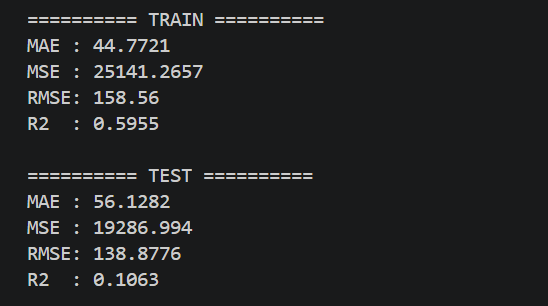
\includegraphics[width=0.6\textwidth]{images/anh_chuong4/random_forest_before_metrics.png}
	\caption{\centering Kết quả mô hình Random Forest trước xử lý ngoại lai}
	\label{fig:rf_before_metrics}
\end{figure}

Nguyên nhân chủ yếu đến từ đặc điểm của bộ dữ liệu Superstore Sales. Một số giao dịch có lợi nhuận quá lớn hoặc quá nhỏ làm tăng độ biến động của biến Profit và ảnh hưởng đến quá trình xây dựng cây quyết định.

Mặc dù Random Forest ít nhạy cảm với ngoại lai hơn hồi quy tuyến tính, mô hình vẫn có thể bị ảnh hưởng khi dữ liệu tồn tại nhiều giá trị cực đoan. Một số cây quyết định có xu hướng học quá chi tiết từ các giao dịch bất thường, làm giảm khả năng tổng quát hóa trên tập kiểm tra.

\begin{figure}[H]
	\centering
	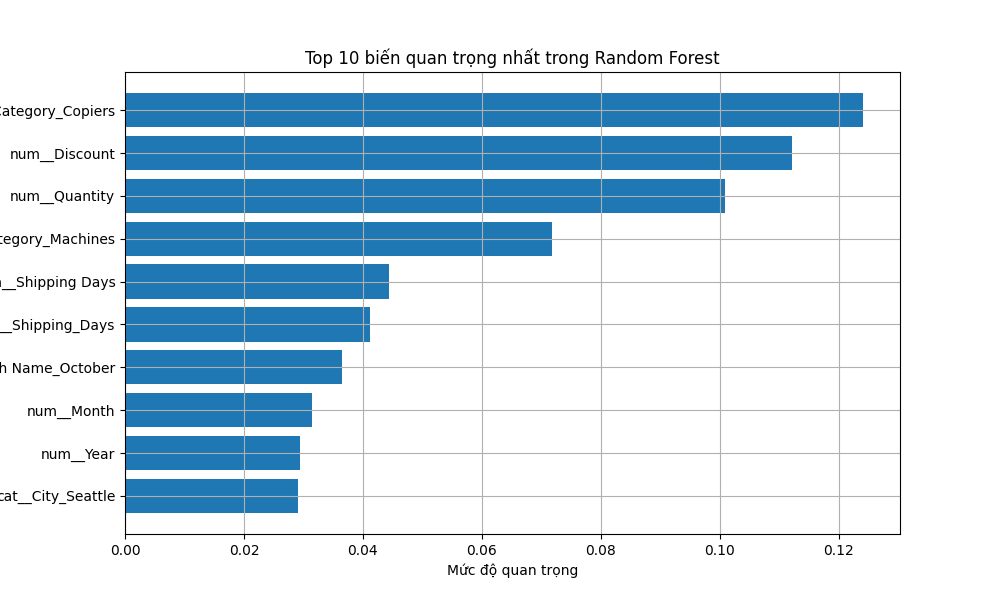
\includegraphics[width=0.8\textwidth]{images/anh_chuong4/random_forest_feature_importance.png}
	\caption{\centering Mức độ quan trọng của các biến trước khi xử lý ngoại lai}
	\label{fig:rf_importance_after_clean}
\end{figure}

Quan sát Hình \ref{fig:rf_importance_after_clean} cho thấy các biến như Discount, Quantity và một số nhóm sản phẩm có ảnh hưởng lớn đến khả năng dự báo lợi nhuận của mô hình.	

\refstepcounter{subsection}
\subsection*{\thesubsection\quad Kết quả sau xử lý ngoại lai}

Sau khi xử lý ngoại lai bằng phương pháp IQR Capping, hiệu quả của mô hình Random Forest được cải thiện rõ rệt trên cả tập huấn luyện và tập kiểm tra.

Cụ thể:
\begin{itemize}
	\item Tập huấn luyện đạt \(MAE = 10.7544\), \(RMSE = 14.7411\) và \(R^2 = 0.7484\).
	\item Tập kiểm tra đạt \(MAE = 15.49\), \(RMSE = 20.9505\) và \(R^2 = 0.4892\).
\end{itemize}

Giá trị \(R^2\) tăng đáng kể so với trước xử lý ngoại lai, đồng thời các chỉ số MAE và RMSE giảm rõ rệt. Điều này cho thấy việc xử lý ngoại lai giúp mô hình học ổn định hơn và cải thiện khả năng dự báo lợi nhuận.

\begin{figure}[H]
	\centering
	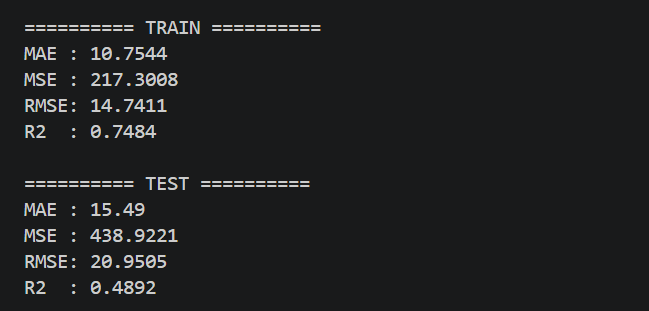
\includegraphics[width=0.6\textwidth]{images/anh_chuong4/random_forest_after_metrics.png}
	\caption{\centering Kết quả mô hình Random Forest sau xử lý ngoại lai}
	\label{fig:rf_after_metrics}
\end{figure}

Nguyên nhân là do các giá trị lợi nhuận quá lớn hoặc quá nhỏ đã được giới hạn trong khoảng hợp lý hơn, giúp các cây quyết định tập trung tốt hơn vào xu hướng chung của dữ liệu thay vì học quá mức từ các giao dịch bất thường.

\begin{figure}[H]
	\centering
	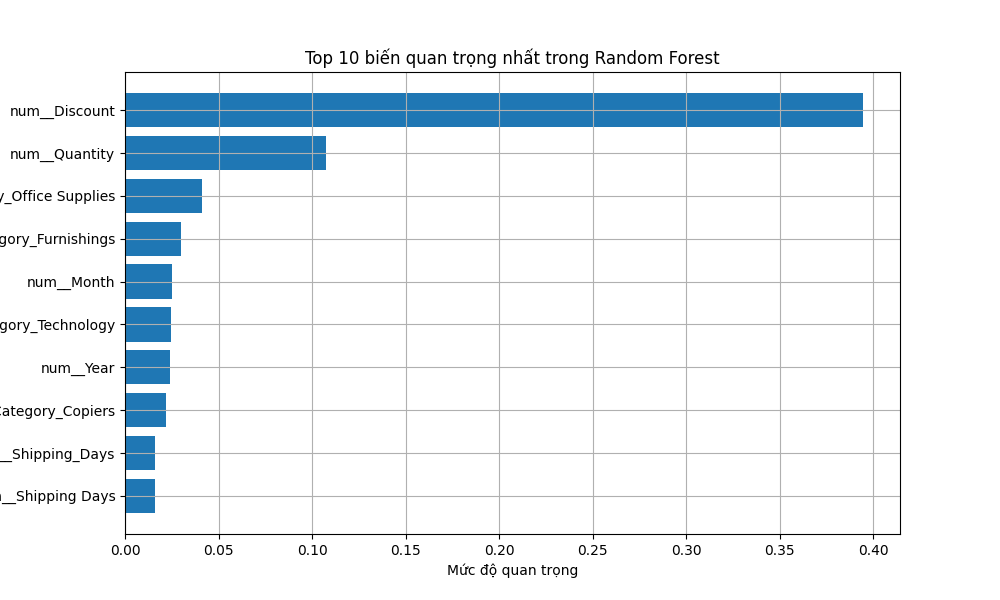
\includegraphics[width=0.8\textwidth]{images/anh_chuong4/random_forest_after_feature_importance.png}
	\caption{\centering Mức độ quan trọng của các biến sau xử lý ngoại lai}
	\label{fig:rf_after_feature_importance}
\end{figure}

Quan sát Hình \ref{fig:rf_after_feature_importance} cho thấy biến Discount có ảnh hưởng lớn nhất đến khả năng dự báo lợi nhuận của mô hình. Ngoài ra, Quantity và một số nhóm sản phẩm cũng có mức độ ảnh hưởng đáng kể, phản ánh lợi nhuận trong dữ liệu bán lẻ chịu tác động mạnh bởi chính sách chiết khấu và đặc điểm sản phẩm.

\refstepcounter{subsection}
\subsection*{\thesubsection\quad So sánh trước và sau xử lý ngoại lai}

Sau khi xử lý ngoại lai, hiệu quả của mô hình Random Forest được cải thiện rõ rệt. Giá trị \(R^2\) trên tập kiểm tra tăng từ 0.1063 lên 0.4892, đồng thời các chỉ số MAE và RMSE giảm đáng kể so với trước xử lý ngoại lai.

Mặc dù Random Forest có khả năng chống chịu ngoại lai tốt hơn hồi quy tuyến tính, việc xử lý ngoại lai vẫn giúp mô hình học ổn định hơn và nâng cao khả năng tổng quát hóa trên tập kiểm tra. Điều này cho thấy việc làm sạch dữ liệu có vai trò quan trọng trong bài toán dự báo lợi nhuận đối với dữ liệu bán lẻ.

\refstepcounter{subsection}
\subsection*{\thesubsection\quad Nhận xét mô hình}

Random Forest là mô hình cho kết quả khá tốt trong bài toán dự báo lợi nhuận nhờ khả năng học được các quan hệ phi tuyến và tương tác giữa nhiều biến đầu vào. Sau khi xử lý ngoại lai, hiệu quả mô hình được cải thiện đáng kể và tốt hơn nhiều so với hồi quy tuyến tính đa biến.

Ngoài ra, Random Forest còn có ưu điểm trong việc xác định mức độ quan trọng của các biến, qua đó hỗ trợ phân tích các yếu tố ảnh hưởng đến lợi nhuận trong dữ liệu bán lẻ.

\section{Mô hình Gradient Boosting}

\refstepcounter{subsection}
\subsection*{\thesubsection\quad Giới thiệu mô hình}

Gradient Boosting Regressor là mô hình thuộc nhóm boosting. Khác với Random Forest xây dựng nhiều cây tương đối độc lập, Gradient Boosting xây dựng các cây theo cách tuần tự. Mỗi cây mới được huấn luyện nhằm giảm phần sai số mà các cây trước đó chưa dự báo tốt.

Cơ chế này giúp Gradient Boosting có khả năng học sâu hơn các quy luật phức tạp trong dữ liệu. Mô hình đặc biệt phù hợp với dữ liệu dạng bảng, nơi biến mục tiêu chịu ảnh hưởng bởi nhiều yếu tố và các mối quan hệ không hoàn toàn tuyến tính.

\refstepcounter{subsection}
\subsection*{\thesubsection\quad Kết quả trước xử lý ngoại lai}

Trước khi xử lý ngoại lai, mô hình Gradient Boosting cho kết quả chưa tốt trên tập kiểm tra với giá trị \(R^2 = -0.033\). Giá trị \(R^2\) âm cho thấy mô hình dự báo kém hơn cả việc sử dụng giá trị trung bình của biến Profit để dự báo.

Cụ thể:
\begin{itemize}
	\item Tập huấn luyện đạt \(MAE = 55.3735\), \(RMSE = 162.5168\) và \(R^2 = 0.575\).
	\item Tập kiểm tra đạt \(MAE = 57.0017\), \(RMSE = 149.3123\) và \(R^2 = -0.033\).
\end{itemize}

Kết quả này cho thấy tồn tại sự chênh lệch lớn giữa tập huấn luyện và tập kiểm tra. Mô hình học khá tốt trên dữ liệu huấn luyện nhưng chưa tổng quát hóa tốt trên dữ liệu kiểm tra khi dữ liệu vẫn chứa nhiều giá trị ngoại lai.

\begin{figure}[H]
	\centering
	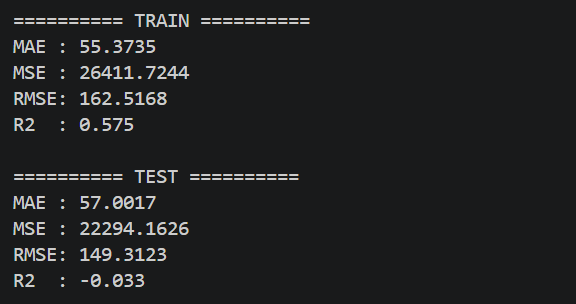
\includegraphics[width=0.6\textwidth]{images/anh_chuong4/gradient_boosting_before_metrics.png}
	\caption{\centering Kết quả mô hình Gradient Boosting trước xử lý ngoại lai}
	\label{fig:gb_before_metrics}
\end{figure}

Nguyên nhân chủ yếu đến từ sự tồn tại của nhiều giá trị ngoại lai trong dữ liệu lợi nhuận. Gradient Boosting là mô hình học tuần tự dựa trên sai số của các bước trước, vì vậy các giao dịch có sai số lớn có thể khiến mô hình tập trung quá mức vào những điểm bất thường.

Điều này làm giảm khả năng học xu hướng chung của dữ liệu và ảnh hưởng đến khả năng tổng quát hóa trên tập kiểm tra.

\begin{figure}[H]
	\centering
	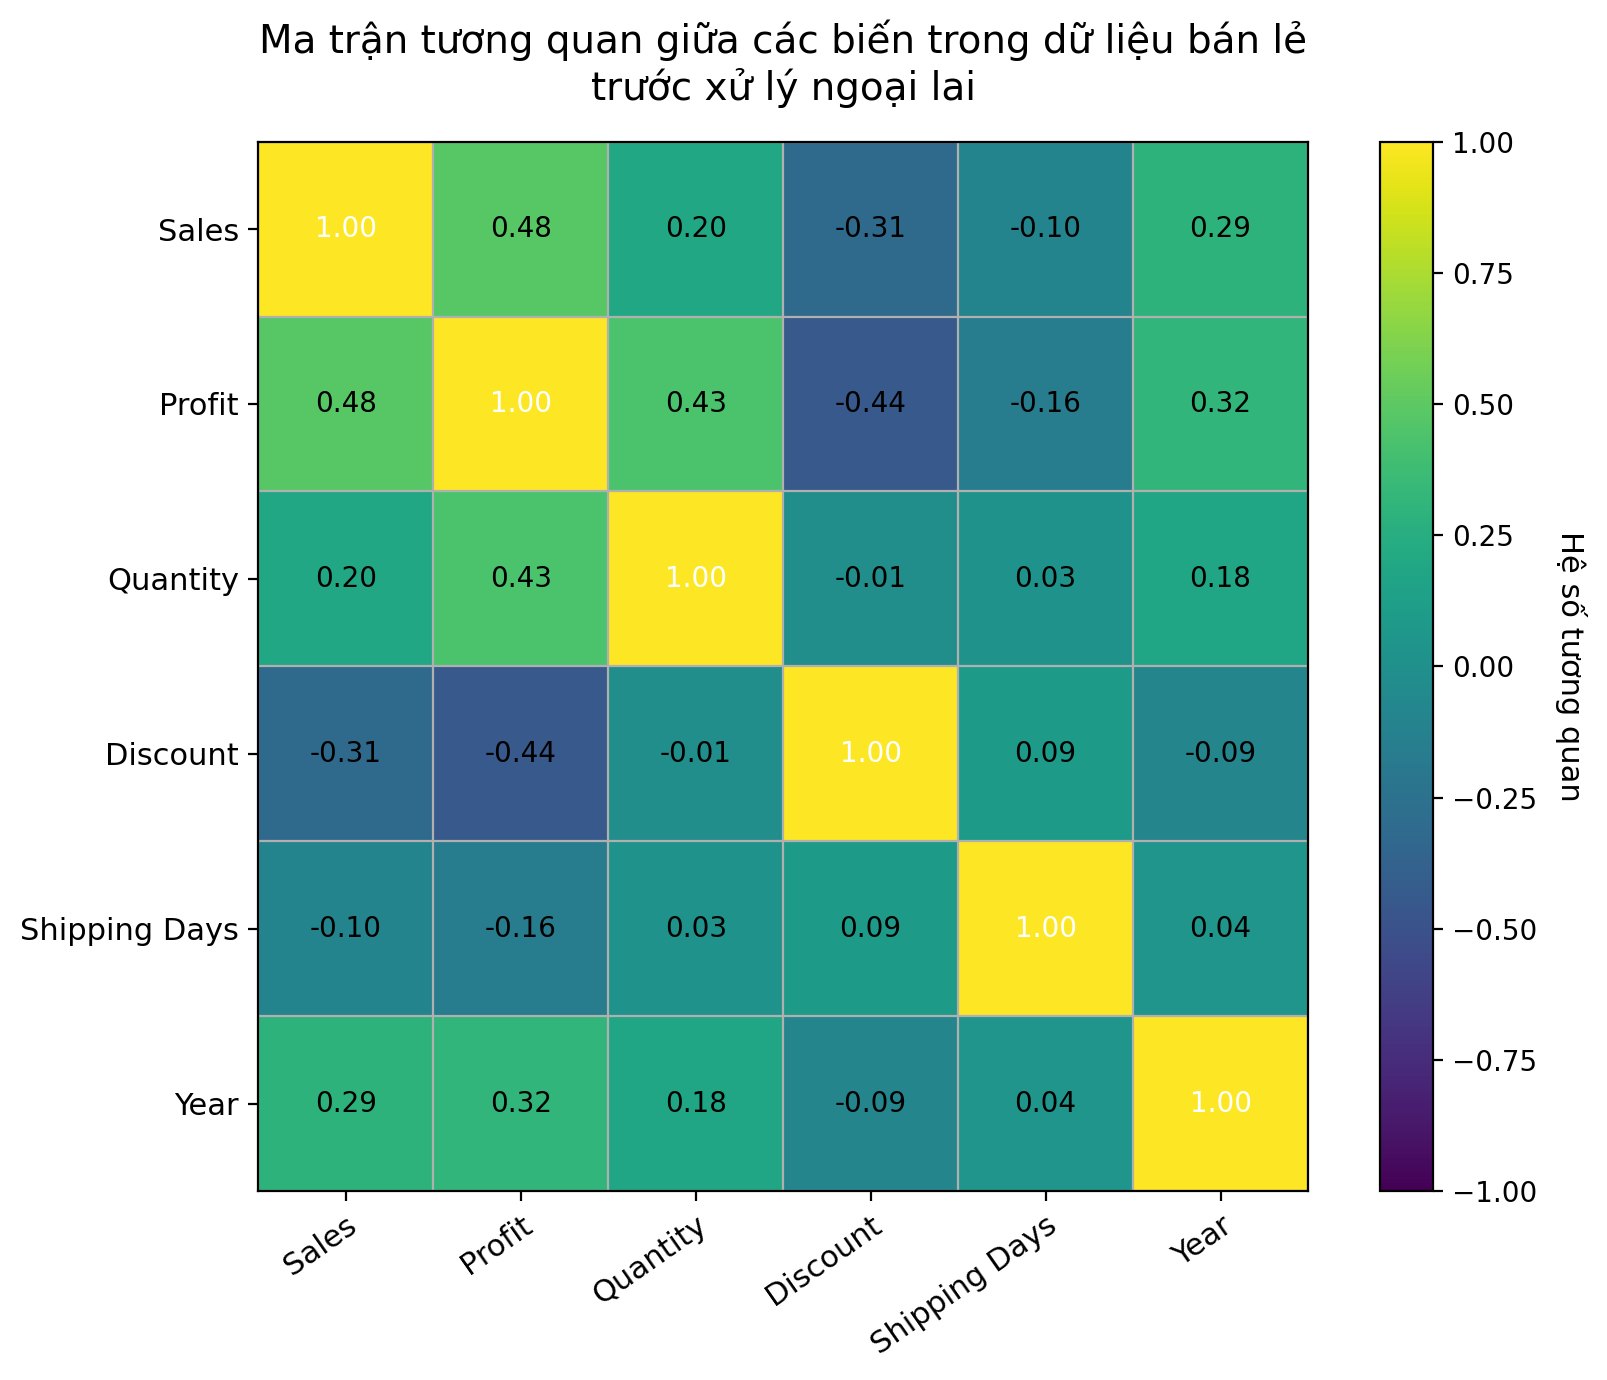
\includegraphics[width=0.8\textwidth]{images/anh_chuong4/Ma_tran_tuong_quan_ban_le.png}
    \caption{\centering Ma trận tương quan giữa các biến số chính trước xử lý ngoại lai}
	\label{fig:gb_before_correlation_matrix}
\end{figure}

Quan sát Hình \ref{fig:gb_before_correlation_matrix} cho thấy các biến trong dữ liệu bán lẻ có mức độ tương quan khác nhau với biến Profit. Trong đó, Discount có tương quan âm với Profit, phản ánh rằng mức chiết khấu cao có thể làm giảm lợi nhuận của doanh nghiệp. Ngược lại, Sales và Quantity có tương quan dương với Profit, cho thấy doanh thu và số lượng bán ra có xu hướng đóng góp tích cực vào lợi nhuận.

Bên cạnh đó, Shipping Days có tương quan yếu với Profit, cho thấy thời gian giao hàng không phải là yếu tố ảnh hưởng mạnh đến lợi nhuận trong bộ dữ liệu này. Biến Year có tương quan dương nhẹ với Profit, phản ánh lợi nhuận có xu hướng cải thiện theo thời gian.

\refstepcounter{subsection}
\subsection*{\thesubsection\quad Kết quả sau xử lý ngoại lai}

Sau khi xử lý ngoại lai bằng phương pháp IQR Capping, hiệu quả của mô hình Gradient Boosting được cải thiện rõ rệt trên cả tập huấn luyện và tập kiểm tra.

Cụ thể:
\begin{itemize}
	\item Tập huấn luyện đạt \(MAE = 15.1713\), \(RMSE = 19.889\) và \(R^2 = 0.542\).
	\item Tập kiểm tra đạt \(MAE = 15.7957\), \(RMSE = 20.652\) và \(R^2 = 0.5036\).
\end{itemize}

Giá trị \(R^2\) trên tập kiểm tra tăng mạnh từ \(-0.033\) lên \(0.5036\), đồng thời các chỉ số MAE và RMSE giảm đáng kể. Điều này cho thấy việc xử lý ngoại lai giúp mô hình học ổn định hơn và nâng cao khả năng dự báo lợi nhuận.

\begin{figure}[H]
	\centering
	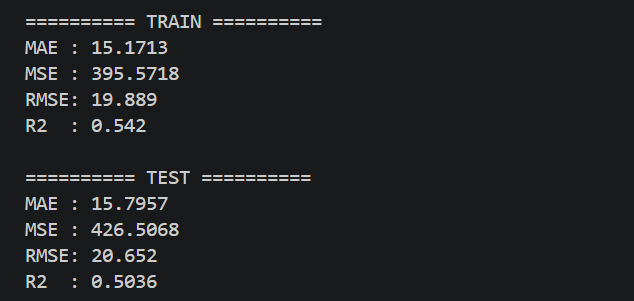
\includegraphics[width=0.6\textwidth]{images/anh_chuong4/gradient_boosting_after_metrics.png}
	\caption{\centering Kết quả mô hình Gradient Boosting sau xử lý ngoại lai}
	\label{fig:gb_after_metrics}
\end{figure}

Nguyên nhân là do các giá trị lợi nhuận bất thường đã được kiểm soát tốt hơn, giúp mô hình không còn tập trung quá mức vào các giao dịch cực đoan. Nhờ đó, Gradient Boosting có thể học hiệu quả hơn các xu hướng chung trong dữ liệu bán lẻ.

Ngoài ra, kết quả của Gradient Boosting sau xử lý ngoại lai cũng cao hơn Random Forest trên tập kiểm tra. Điều này cho thấy cơ chế học tuần tự của boosting có khả năng khai thác tốt các quan hệ phức tạp giữa các biến khi dữ liệu đầu vào được xử lý phù hợp.

\begin{figure}[H]
	\centering
	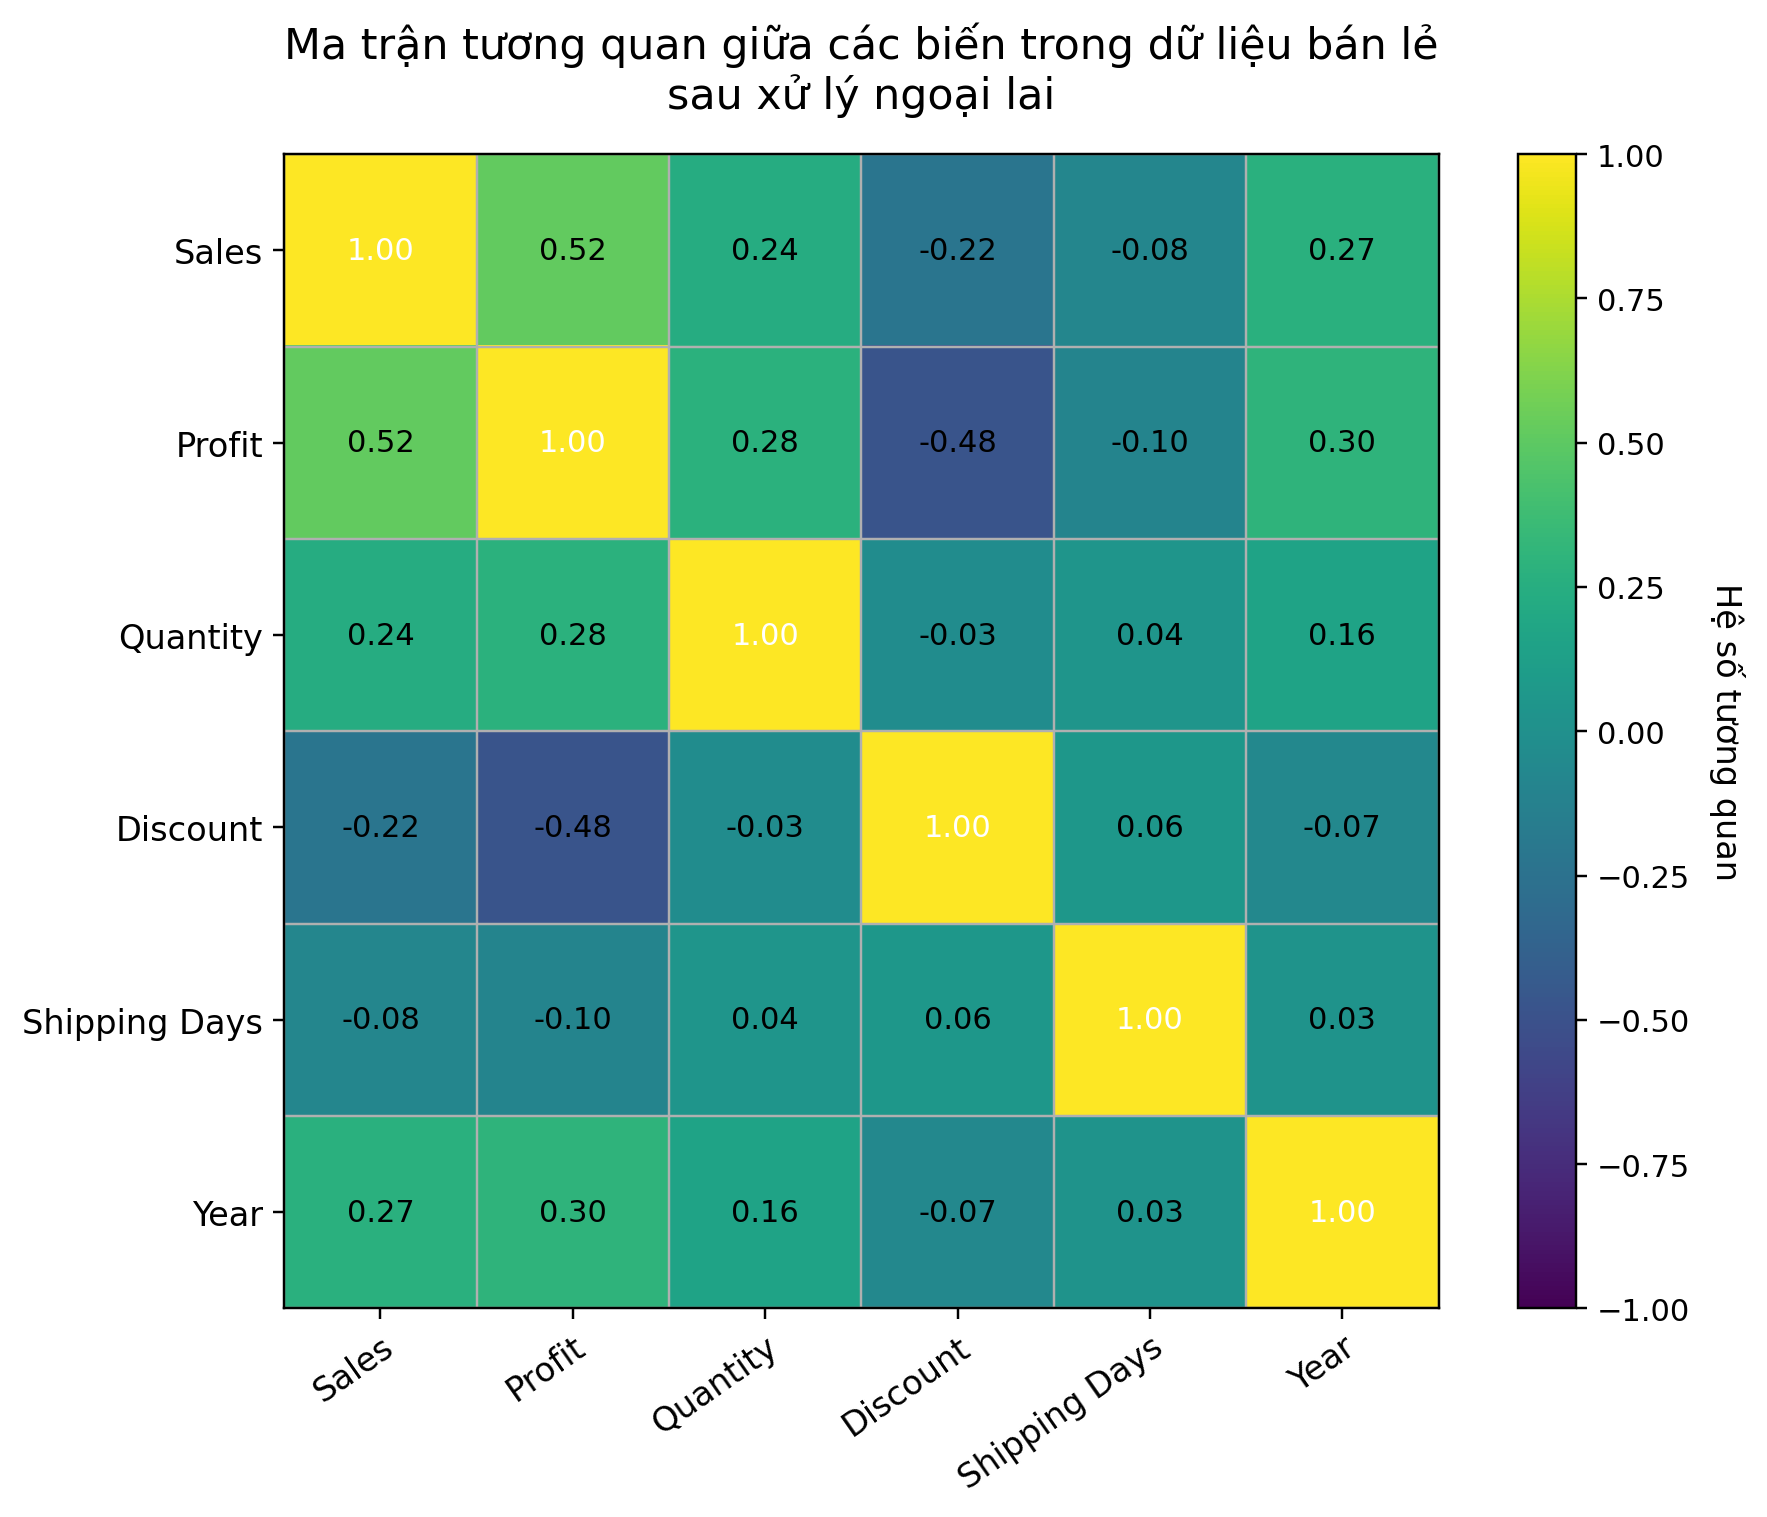
\includegraphics[width=0.85\textwidth]{images/anh_chuong4/Ma_tran_tuong_quan_sau_xu_ly_ngoai_lai.png}
    \caption{\centering Ma trận tương quan giữa các biến số chính sau xử lý ngoại lai}
	\label{fig:gb_after_correlation_matrix}
\end{figure}

Quan sát Hình \ref{fig:gb_after_correlation_matrix} cho thấy các biến trong dữ liệu bán lẻ vẫn có mức độ tương quan khác nhau với biến Profit sau khi xử lý ngoại lai. Trong đó, Discount tiếp tục có tương quan âm với Profit, phản ánh rằng mức chiết khấu cao vẫn có xu hướng làm giảm lợi nhuận của doanh nghiệp. Ngược lại, Sales và Quantity có tương quan dương với Profit, cho thấy doanh thu và số lượng bán ra vẫn là những yếu tố đóng góp tích cực vào lợi nhuận.

Ngoài ra, Shipping Days có tương quan yếu với Profit, cho thấy thời gian giao hàng không phải là yếu tố ảnh hưởng mạnh đến lợi nhuận trong bộ dữ liệu này. Biến Year có tương quan dương nhẹ với Profit, phản ánh lợi nhuận có xu hướng cải thiện theo thời gian sau khi dữ liệu đã được làm sạch.


\refstepcounter{subsection}
\subsection*{\thesubsection\quad So sánh trước và sau xử lý ngoại lai}

Gradient Boosting là mô hình có sự cải thiện rõ rệt sau khi xử lý ngoại lai. Giá trị \(R^2\) trên tập kiểm tra tăng từ \(-0.033\) lên \(0.5036\), đồng thời MAE và RMSE giảm đáng kể.

Kết quả này cho thấy mô hình boosting khá nhạy cảm với các giá trị ngoại lai trong dữ liệu. Khi dữ liệu chưa được xử lý, mô hình dễ tập trung quá mức vào các giao dịch bất thường. Sau khi làm sạch dữ liệu, Gradient Boosting học ổn định hơn và khai thác tốt các quan hệ phi tuyến giữa các biến, từ đó nâng cao hiệu quả dự báo.

\refstepcounter{subsection}
\subsection*{\thesubsection\quad Nhận xét mô hình}

Gradient Boosting cho kết quả tốt sau khi xử lý ngoại lai và có khả năng tổng quát hóa tương đối ổn định trên tập kiểm tra. Mô hình phù hợp với bài toán dự báo lợi nhuận nhờ khả năng học được các quan hệ phi tuyến và tương tác phức tạp giữa nhiều biến đầu vào.

Tuy nhiên, mô hình khá nhạy cảm với các giá trị ngoại lai do cơ chế học tuần tự dựa trên sai số. Nếu dữ liệu chứa nhiều điểm bất thường, mô hình có thể tập trung quá mức vào các giao dịch ngoại lệ và làm giảm hiệu quả dự báo. Vì vậy, bước xử lý ngoại lai đóng vai trò quan trọng trong việc nâng cao hiệu quả của Gradient Boosting trong đề tài này.

\section{Mô hình XGBoost}

\refstepcounter{subsection}
\subsection*{\thesubsection\quad Giới thiệu mô hình}

XGBoost Regressor là mô hình boosting nâng cao, được phát triển nhằm cải thiện hiệu quả dự báo và tốc độ huấn luyện. Mô hình vẫn dựa trên nguyên lý xây dựng các cây quyết định theo cách tuần tự, nhưng bổ sung thêm cơ chế để kiểm soát độ phức tạp của mô hình và hạn chế hiện tượng quá khớp.

XGBoost thường cho kết quả tốt đối với dữ liệu dạng bảng, đặc biệt trong các bài toán dự báo có nhiều biến định tính sau khi mã hóa. Sau khi được mã hóa bằng One-Hot Encoding, các biến này tạo thành tập đặc trưng dạng bảng phù hợp với XGBoost.

\refstepcounter{subsection}
\subsection*{\thesubsection\quad Kết quả trước xử lý ngoại lai}

Trước khi xử lý ngoại lai, mô hình XGBoost cho kết quả tốt hơn hồi quy tuyến tính đa biến và Gradient Boosting trên tập kiểm tra với giá trị \(R^2 = 0.1204\). Điều này cho thấy XGBoost có khả năng học dữ liệu tốt hơn ngay cả khi dữ liệu còn chứa nhiều nhiễu và giá trị bất thường.

Cụ thể:
\begin{itemize}
	\item Tập huấn luyện đạt \(MAE = 49.3776\), \(RMSE = 124.2613\) và \(R^2 = 0.7515\).
	\item Tập kiểm tra đạt \(MAE = 54.7294\), \(RMSE = 137.7825\) và \(R^2 = 0.1204\).
\end{itemize}

Mặc dù kết quả trên tập train khá cao, hiệu quả trên tập test vẫn còn thấp. Điều này cho thấy mô hình có dấu hiệu overfitting và vẫn chịu ảnh hưởng bởi các giá trị ngoại lai trong dữ liệu lợi nhuận.

\begin{figure}[H]
	\centering
	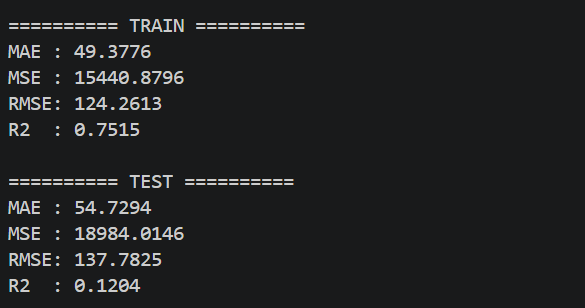
\includegraphics[width=0.6\textwidth]{images/anh_chuong4/xgboost_before_metrics.png}
	\caption{\centering Kết quả mô hình XGBoost trước xử lý ngoại lai}
	\label{fig:xgb_before_metrics}
\end{figure}

Nguyên nhân chủ yếu đến từ các giao dịch có lợi nhuận quá lớn hoặc quá nhỏ làm tăng độ biến động của biến Profit. Các giá trị ngoại lai khiến mô hình khó học chính xác xu hướng chung của dữ liệu và làm giảm khả năng tổng quát hóa trên tập kiểm tra.

Mặc dù XGBoost có cơ chế regularization giúp hạn chế overfitting tốt hơn nhiều mô hình khác, mô hình vẫn không thể loại bỏ hoàn toàn ảnh hưởng của dữ liệu bất thường nếu ngoại lai xuất hiện với mức độ lớn.

\begin{figure}[H]
	\centering
	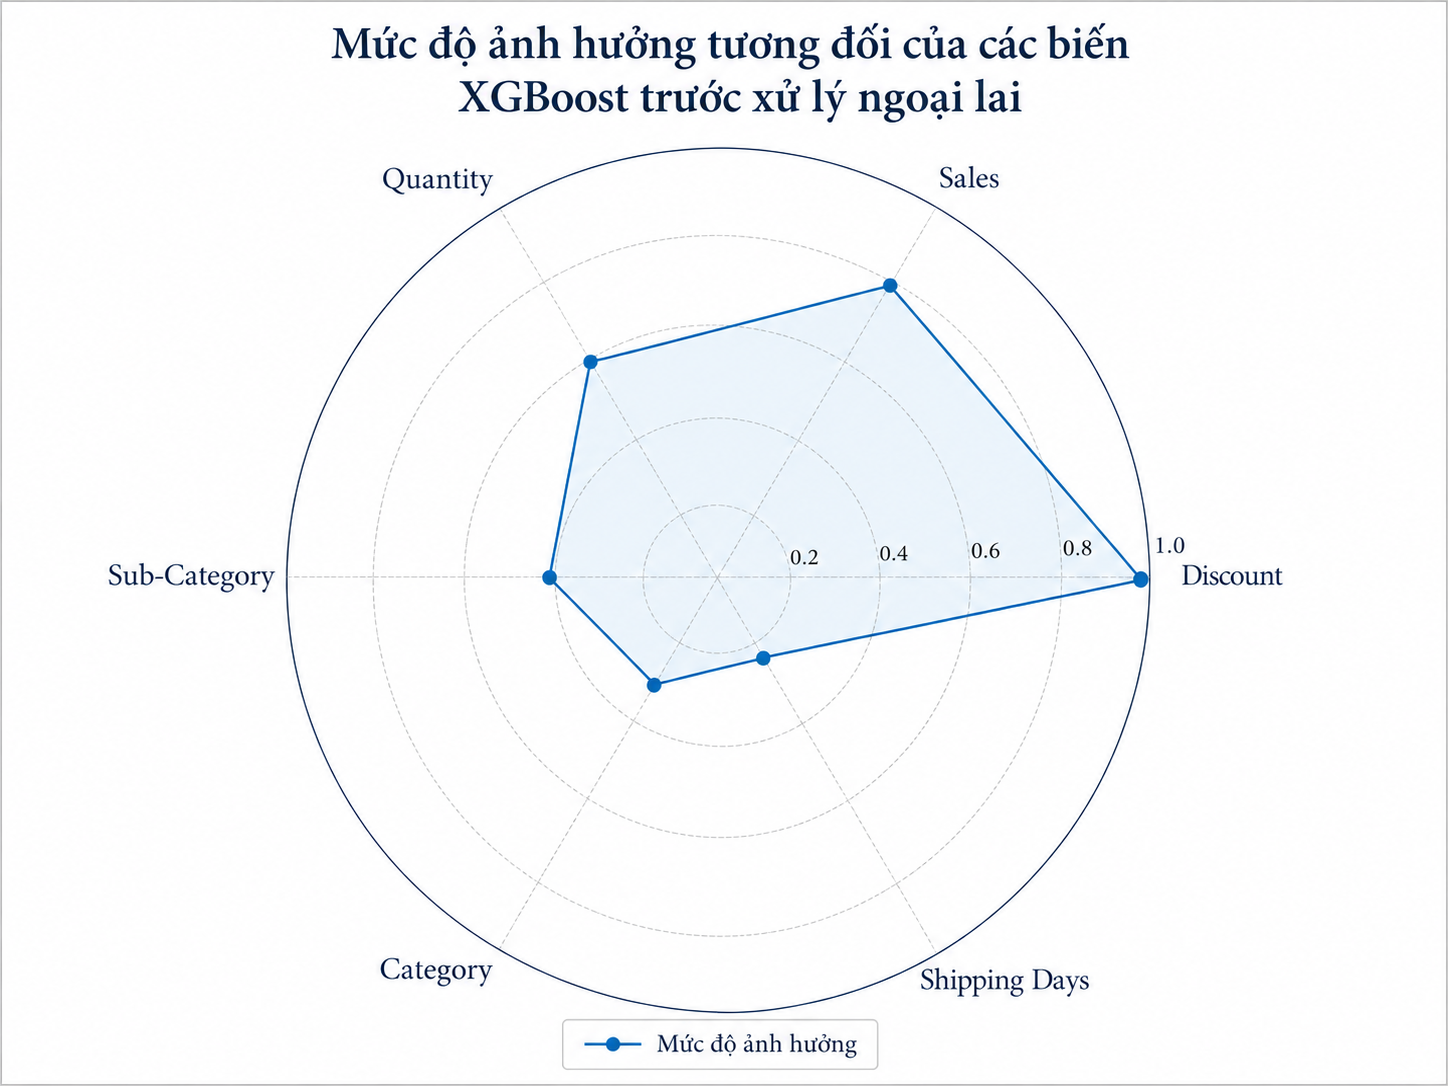
\includegraphics[width=0.8\textwidth]{images/anh_chuong4/1.png}
	\caption{\centering Mức độ ảnh hưởng của các biến trước xử lý ngoại lai}
	\label{fig:xgb_before_radar_importance}
\end{figure}

Quan sát Hình \ref{fig:xgb_before_radar_importance} cho thấy Discount là biến có mức độ ảnh hưởng lớn nhất trong mô hình XGBoost trước xử lý ngoại lai. Điều này cho thấy chính sách chiết khấu có vai trò quan trọng trong việc dự báo lợi nhuận của doanh nghiệp.

Bên cạnh đó, Sales và Quantity cũng có mức độ ảnh hưởng tương đối cao, phản ánh rằng doanh thu và số lượng bán ra là các yếu tố liên quan trực tiếp đến lợi nhuận. Các biến như Sub-Category, Category và Shipping Days có mức độ ảnh hưởng thấp hơn, nhưng vẫn góp phần bổ sung thông tin cho mô hình trong quá trình dự báo.

\refstepcounter{subsection}
\subsection*{\thesubsection\quad Kết quả sau xử lý ngoại lai}

Sau khi xử lý ngoại lai, mô hình XGBoost cho kết quả tốt nhất trong các mô hình dự báo lợi nhuận. Giá trị \(R^2\) trên tập kiểm tra tăng đáng kể lên khoảng 0.5109, đồng thời các chỉ số MAE và RMSE giảm rõ rệt.

Cụ thể:
\begin{itemize}
	\item Tập huấn luyện đạt \(MAE = 14.4558\), \(RMSE = 19.0851\) và \(R^2 = 0.5782\).
	\item Tập kiểm tra đạt \(MAE = 15.5767\), \(RMSE = 20.5\) và \(R^2 = 0.5109\).
\end{itemize}

Kết quả này cho thấy XGBoost có khả năng học hiệu quả các quan hệ phi tuyến và các tương tác phức tạp giữa nhiều biến trong dữ liệu bán lẻ.

\begin{figure}[H]
	\centering
	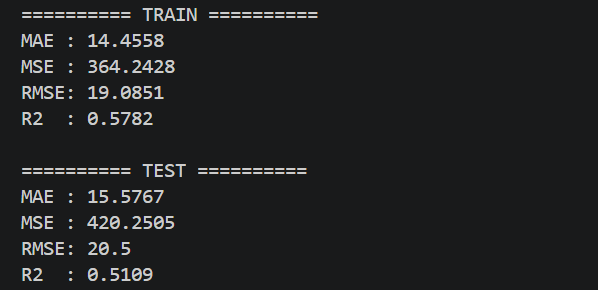
\includegraphics[width=0.6\textwidth]{images/anh_chuong4/xgboost_after_metrics.png}
	\caption{\centering Kết quả mô hình XGBoost sau xử lý ngoại lai}
	\label{fig:xgb_after_metrics}
\end{figure}

Sau khi các giá trị ngoại lai được kiểm soát, mô hình không còn bị ảnh hưởng quá mạnh bởi các giao dịch cực đoan. Điều này giúp quá trình học diễn ra ổn định hơn và nâng cao khả năng tổng quát hóa trên tập kiểm tra.

Ngoài ra, XGBoost cũng cho kết quả tốt hơn Random Forest và Gradient Boosting sau xử lý ngoại lai. Điều này cho thấy cơ chế boosting kết hợp regularization của XGBoost phù hợp với dữ liệu bán lẻ và có khả năng khai thác tốt các đặc trưng quan trọng trong dữ liệu.

\begin{figure}[H]
	\centering
	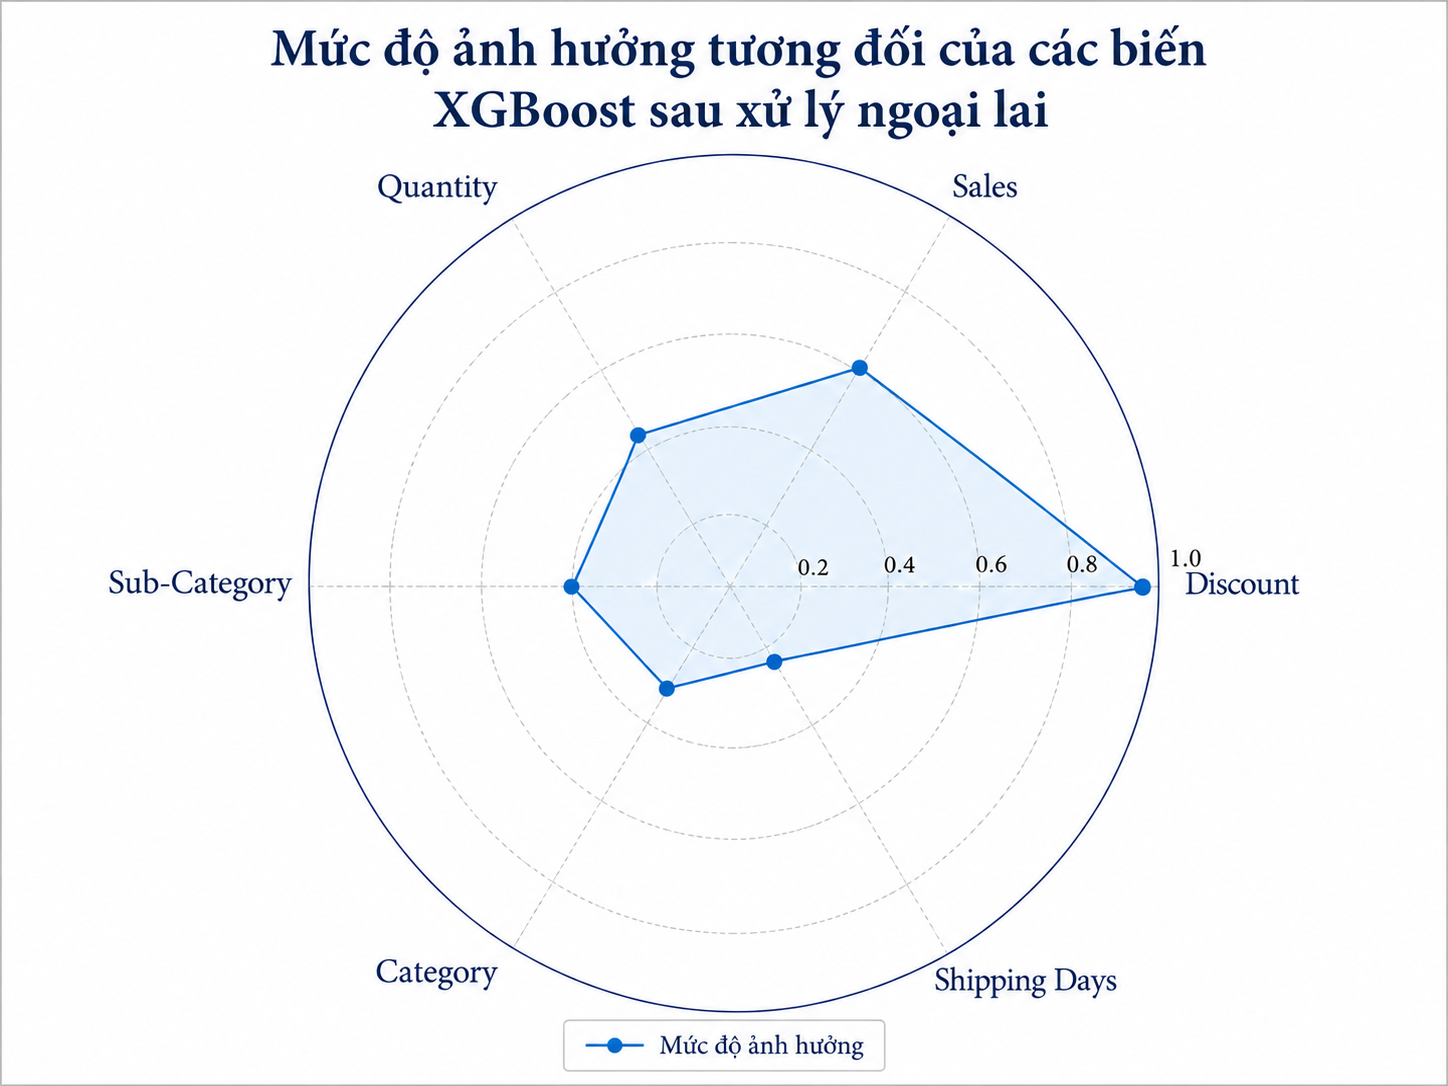
\includegraphics[width=0.8\textwidth]{images/anh_chuong4/2.png}
    \caption{\centering Mức độ ảnh hưởng của các biến sau xử lý ngoại lai}
	\label{fig:xgb_after_importance}
\end{figure}

Quan sát Hình \ref{fig:xgb_after_importance} cho thấy Discount tiếp tục là biến có mức độ ảnh hưởng lớn nhất đến khả năng dự báo lợi nhuận của mô hình XGBoost sau khi xử lý ngoại lai. Bên cạnh đó, một số biến thuộc nhóm sản phẩm và khu vực cũng có vai trò đáng kể trong quá trình dự báo. Kết quả này cho thấy lợi nhuận trong dữ liệu bán lẻ không chỉ chịu tác động mạnh bởi chính sách chiết khấu mà còn phụ thuộc vào đặc điểm sản phẩm và yếu tố thị trường ở từng khu vực.

\refstepcounter{subsection}
\subsection*{\thesubsection\quad So sánh trước và sau xử lý ngoại lai}

Sau khi xử lý ngoại lai, hiệu quả của mô hình XGBoost được cải thiện rõ rệt. Giá trị \(R^2\) trên tập kiểm tra tăng từ 0.1204 lên 0.5109, đồng thời các chỉ số MAE và RMSE giảm đáng kể so với trước xử lý ngoại lai.

Mặc dù XGBoost vốn đã có khả năng xử lý dữ liệu phức tạp và hạn chế overfitting khá tốt, các giá trị ngoại lai vẫn ảnh hưởng đáng kể đến khả năng dự báo của mô hình. Sau khi dữ liệu được làm sạch, mô hình học ổn định hơn và nâng cao khả năng tổng quát hóa trên tập kiểm tra.

Kết quả này cho thấy xử lý ngoại lai là bước quan trọng giúp XGBoost phát huy tốt hơn hiệu quả dự báo trong bài toán dữ liệu bán lẻ.

\refstepcounter{subsection}
\subsection*{\thesubsection\quad Nhận xét mô hình}

XGBoost là mô hình cho kết quả tốt nhất trong bài toán dự báo lợi nhuận của đề tài. Mô hình đạt giá trị \(R^2\) cao nhất trên tập kiểm tra và có các chỉ số sai số thấp hơn so với các mô hình còn lại.

Ưu điểm của XGBoost nằm ở khả năng học các quan hệ phi tuyến, xử lý hiệu quả dữ liệu dạng bảng và kiểm soát độ phức tạp của mô hình thông qua cơ chế regularization. Điều này giúp mô hình phù hợp với dữ liệu bán lẻ vốn có nhiều mối quan hệ và tương tác phức tạp giữa các biến.

Từ kết quả thực nghiệm, có thể thấy XGBoost là mô hình phù hợp nhất trong phạm vi dữ liệu và phương pháp triển khai của đề tài.


\section{Mô hình K-Means Clustering}

\refstepcounter{subsection}
\subsection*{\thesubsection\quad Giới thiệu mô hình}

K-Means Clustering là mô hình học không giám sát được sử dụng để phân nhóm các đối tượng dựa trên mức độ tương đồng giữa chúng. Khác với các mô hình hồi quy, K-Means không sử dụng biến mục tiêu mà tập trung vào việc tìm ra các nhóm dữ liệu có đặc điểm gần giống nhau.

Trong đề tài, K-Means được sử dụng để phân cụm khách hàng theo đặc điểm tiêu dùng. Dữ liệu được tổng hợp theo từng khách hàng, sau đó xây dựng các biến đặc trưng như tổng doanh thu, tổng lợi nhuận, tổng số lượng mua, số đơn hàng, doanh thu trung bình mỗi đơn, lợi nhuận trung bình mỗi đơn và tỷ suất lợi nhuận.

Các biến sử dụng cho phân cụm gồm:
\begin{itemize}
    \item Total Sales
    \item Total Profit
    \item Total Quantity
    \item Avg Discount
    \item Avg Shipping Days
    \item Order Count
    \item Sales Per Order
    \item Profit Per Order
    \item Profit Margin
\end{itemize}

Trước khi phân cụm, dữ liệu được chuẩn hóa bằng StandardScaler. Đây là bước cần thiết vì các biến có đơn vị đo khác nhau. Nếu không chuẩn hóa, các biến có giá trị lớn như Total Sales hoặc Total Profit có thể chi phối toàn bộ quá trình phân cụm.

\refstepcounter{subsection}
\subsection*{\thesubsection\quad Kết quả trước xử lý ngoại lai}

Trước khi xử lý ngoại lai, dữ liệu khách hàng vẫn tồn tại một số quan sát có tổng doanh thu hoặc tổng lợi nhuận rất lớn so với phần còn lại. Do K-Means sử dụng khoảng cách Euclid để phân nhóm, các giá trị bất thường này có thể làm lệch vị trí tâm cụm và ảnh hưởng đến chất lượng phân cụm.

Kết quả đánh giá số cụm cho thấy tại \(K = 2\), mô hình đạt Silhouette Score khoảng 0.2602. Đây là giá trị cao nhất trong các số cụm được thử nghiệm, vì vậy đề tài lựa chọn \(K = 2\) để thực hiện phân cụm khách hàng trước xử lý ngoại lai.

\begin{figure}[H]
	\centering
	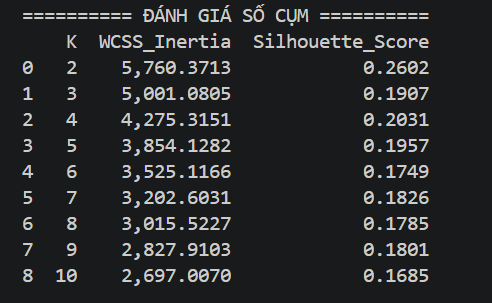
\includegraphics[width=0.6\textwidth]{images/anh_chuong4/kmeans_before_metrics.png}
	\caption{\centering Kết quả đánh giá số cụm K-Means trước xử lý ngoại lai}
	\label{fig:kmeans_before_metrics}
\end{figure}

\begin{figure}[H]
	\centering
	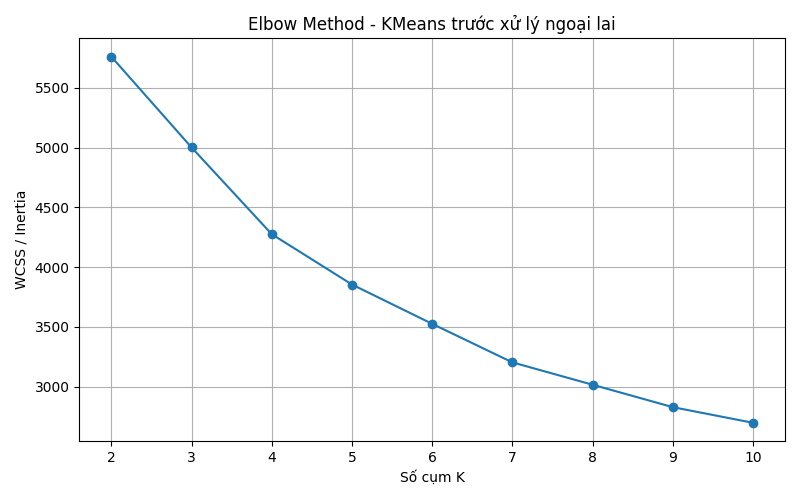
\includegraphics[width=0.7\textwidth]{images/anh_chuong4/kmeans_before_elbow.png}
	\caption{\centering Elbow Method của mô hình K-Means trước xử lý ngoại lai}
	\label{fig:kmeans_before_elbow}
\end{figure}

\begin{figure}[H]
	\centering
	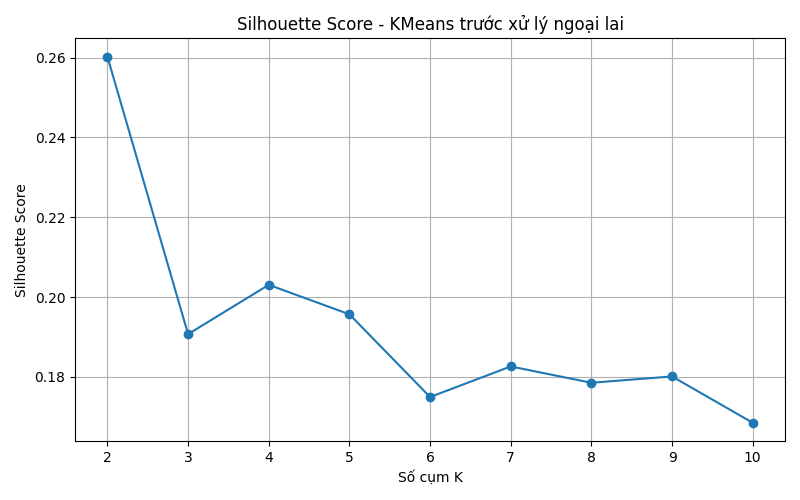
\includegraphics[width=0.7\textwidth]{images/anh_chuong4/kmeans_before_silhouette.png}
	\caption{\centering Silhouette Score của mô hình K-Means trước xử lý ngoại lai}
	\label{fig:kmeans_before_silhouette}
\end{figure}

Quan sát Hình \ref{fig:kmeans_before_elbow} và Hình \ref{fig:kmeans_before_silhouette} cho thấy WCSS giảm dần khi số cụm tăng, trong khi Silhouette Score đạt giá trị cao nhất tại \(K = 2\). Vì vậy, số cụm \(K = 2\) được lựa chọn để phân nhóm khách hàng.

\begin{figure}[H]
	\centering
	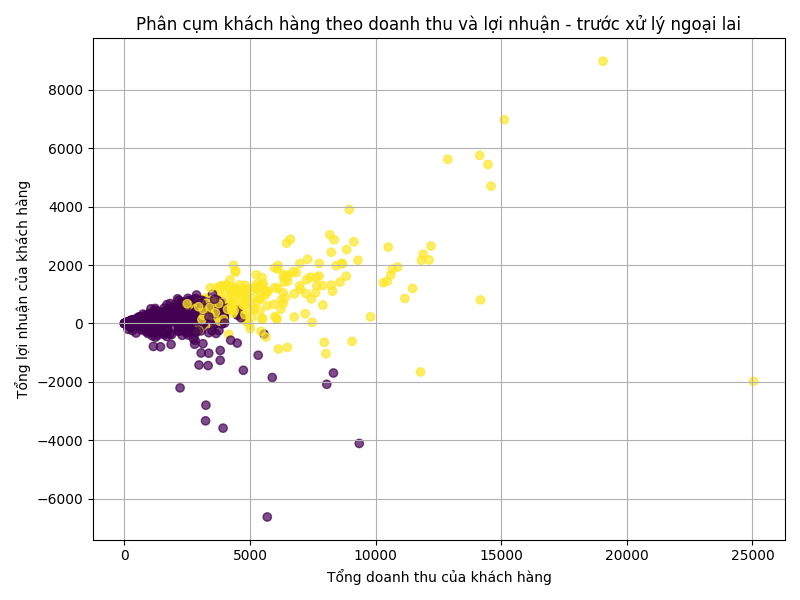
\includegraphics[width=0.8\textwidth]{images/anh_chuong4/kmeans_before_cluster.png}
	\caption{\centering Phân cụm khách hàng trước xử lý ngoại lai}
	\label{fig:kmeans_before_cluster}
\end{figure}

Quan sát Hình \ref{fig:kmeans_before_cluster} cho thấy một số khách hàng có doanh thu hoặc lợi nhuận rất lớn nằm cách xa phần lớn dữ liệu. Các điểm này có thể kéo tâm cụm lệch khỏi vị trí đại diện cho nhóm khách hàng phổ biến, làm giảm tính ổn định của mô hình phân cụm.

\begin{figure}[H]
	\centering
	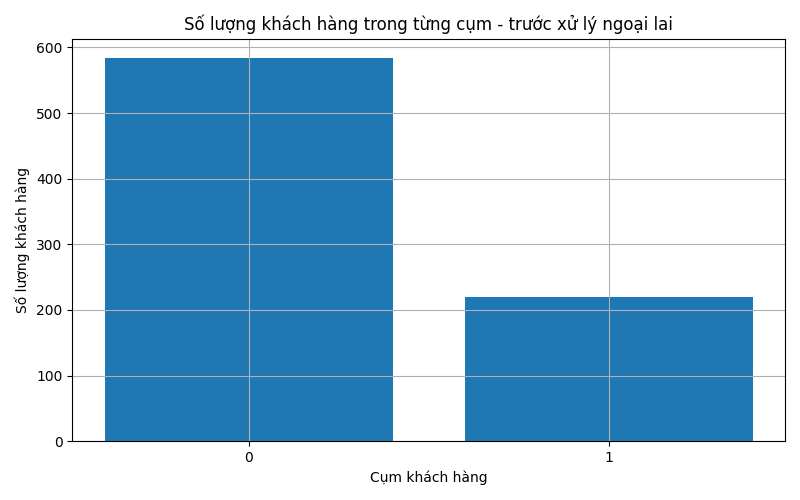
\includegraphics[width=0.65\textwidth]{images/anh_chuong4/kmeans_before_cluster_count.png}
	\caption{\centering Số lượng khách hàng trong từng cụm trước xử lý ngoại lai}
	\label{fig:kmeans_before_cluster_count}
\end{figure}

Biểu đồ số lượng khách hàng cho thấy hai cụm có quy mô không đồng đều. Cụm 0 chiếm phần lớn số lượng khách hàng, trong khi cụm 1 có số lượng ít hơn nhưng thường đại diện cho nhóm khách hàng có giá trị giao dịch cao hơn.

\begin{figure}[H]
	\centering
	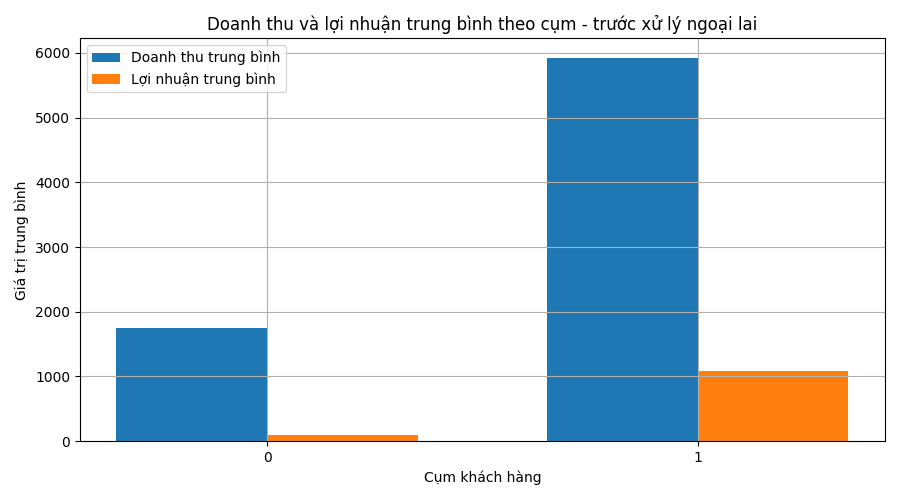
\includegraphics[width=0.75\textwidth]{images/anh_chuong4/kmeans_before_cluster_mean.png}
	\caption{\centering Doanh thu, lợi nhuận trung bình theo cụm trước xử lý ngoại lai}
	\label{fig:kmeans_before_cluster_mean}
\end{figure}

Kết quả doanh thu và lợi nhuận trung bình theo cụm cho thấy cụm 1 có giá trị trung bình cao hơn rõ rệt so với cụm 0. Tuy nhiên, do dữ liệu vẫn còn ngoại lai, kết quả phân cụm có thể bị ảnh hưởng bởi một số khách hàng có doanh thu hoặc lợi nhuận bất thường.

Nhìn chung, trước khi xử lý ngoại lai, K-Means vẫn có thể phân cụm khách hàng thành các nhóm khác nhau. Tuy nhiên, mức độ tách biệt giữa các cụm chưa cao và kết quả còn chịu ảnh hưởng bởi các giá trị cực đoan trong dữ liệu.

\refstepcounter{subsection}
\subsection*{\thesubsection\quad Kết quả sau xử lý ngoại lai}

Sau khi xử lý ngoại lai, dữ liệu khách hàng trở nên ổn định hơn do các giá trị doanh thu và lợi nhuận quá lớn hoặc quá nhỏ đã được giới hạn trong khoảng hợp lý. Điều này giúp mô hình K-Means giảm ảnh hưởng của các điểm cực đoan và xác định tâm cụm chính xác hơn.

Kết quả đánh giá số cụm sau xử lý ngoại lai cho thấy Silhouette Score đạt giá trị cao nhất tại \(K = 2\), với giá trị khoảng 0.2684. Vì vậy, đề tài lựa chọn \(K = 2\) để thực hiện phân cụm khách hàng sau xử lý ngoại lai.

\begin{figure}[H]
	\centering
	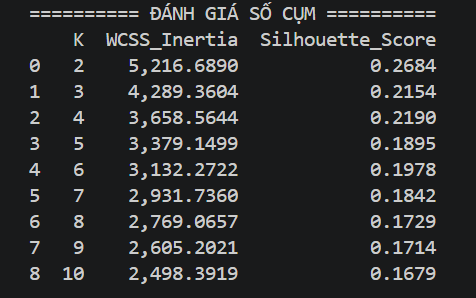
\includegraphics[width=0.6\textwidth]{images/anh_chuong4/kmeans_after_metrics.png}
	\caption{\centering Kết quả đánh giá số cụm K-Means sau xử lý ngoại lai}
	\label{fig:kmeans_after_metrics}
\end{figure}

\begin{figure}[H]
	\centering
	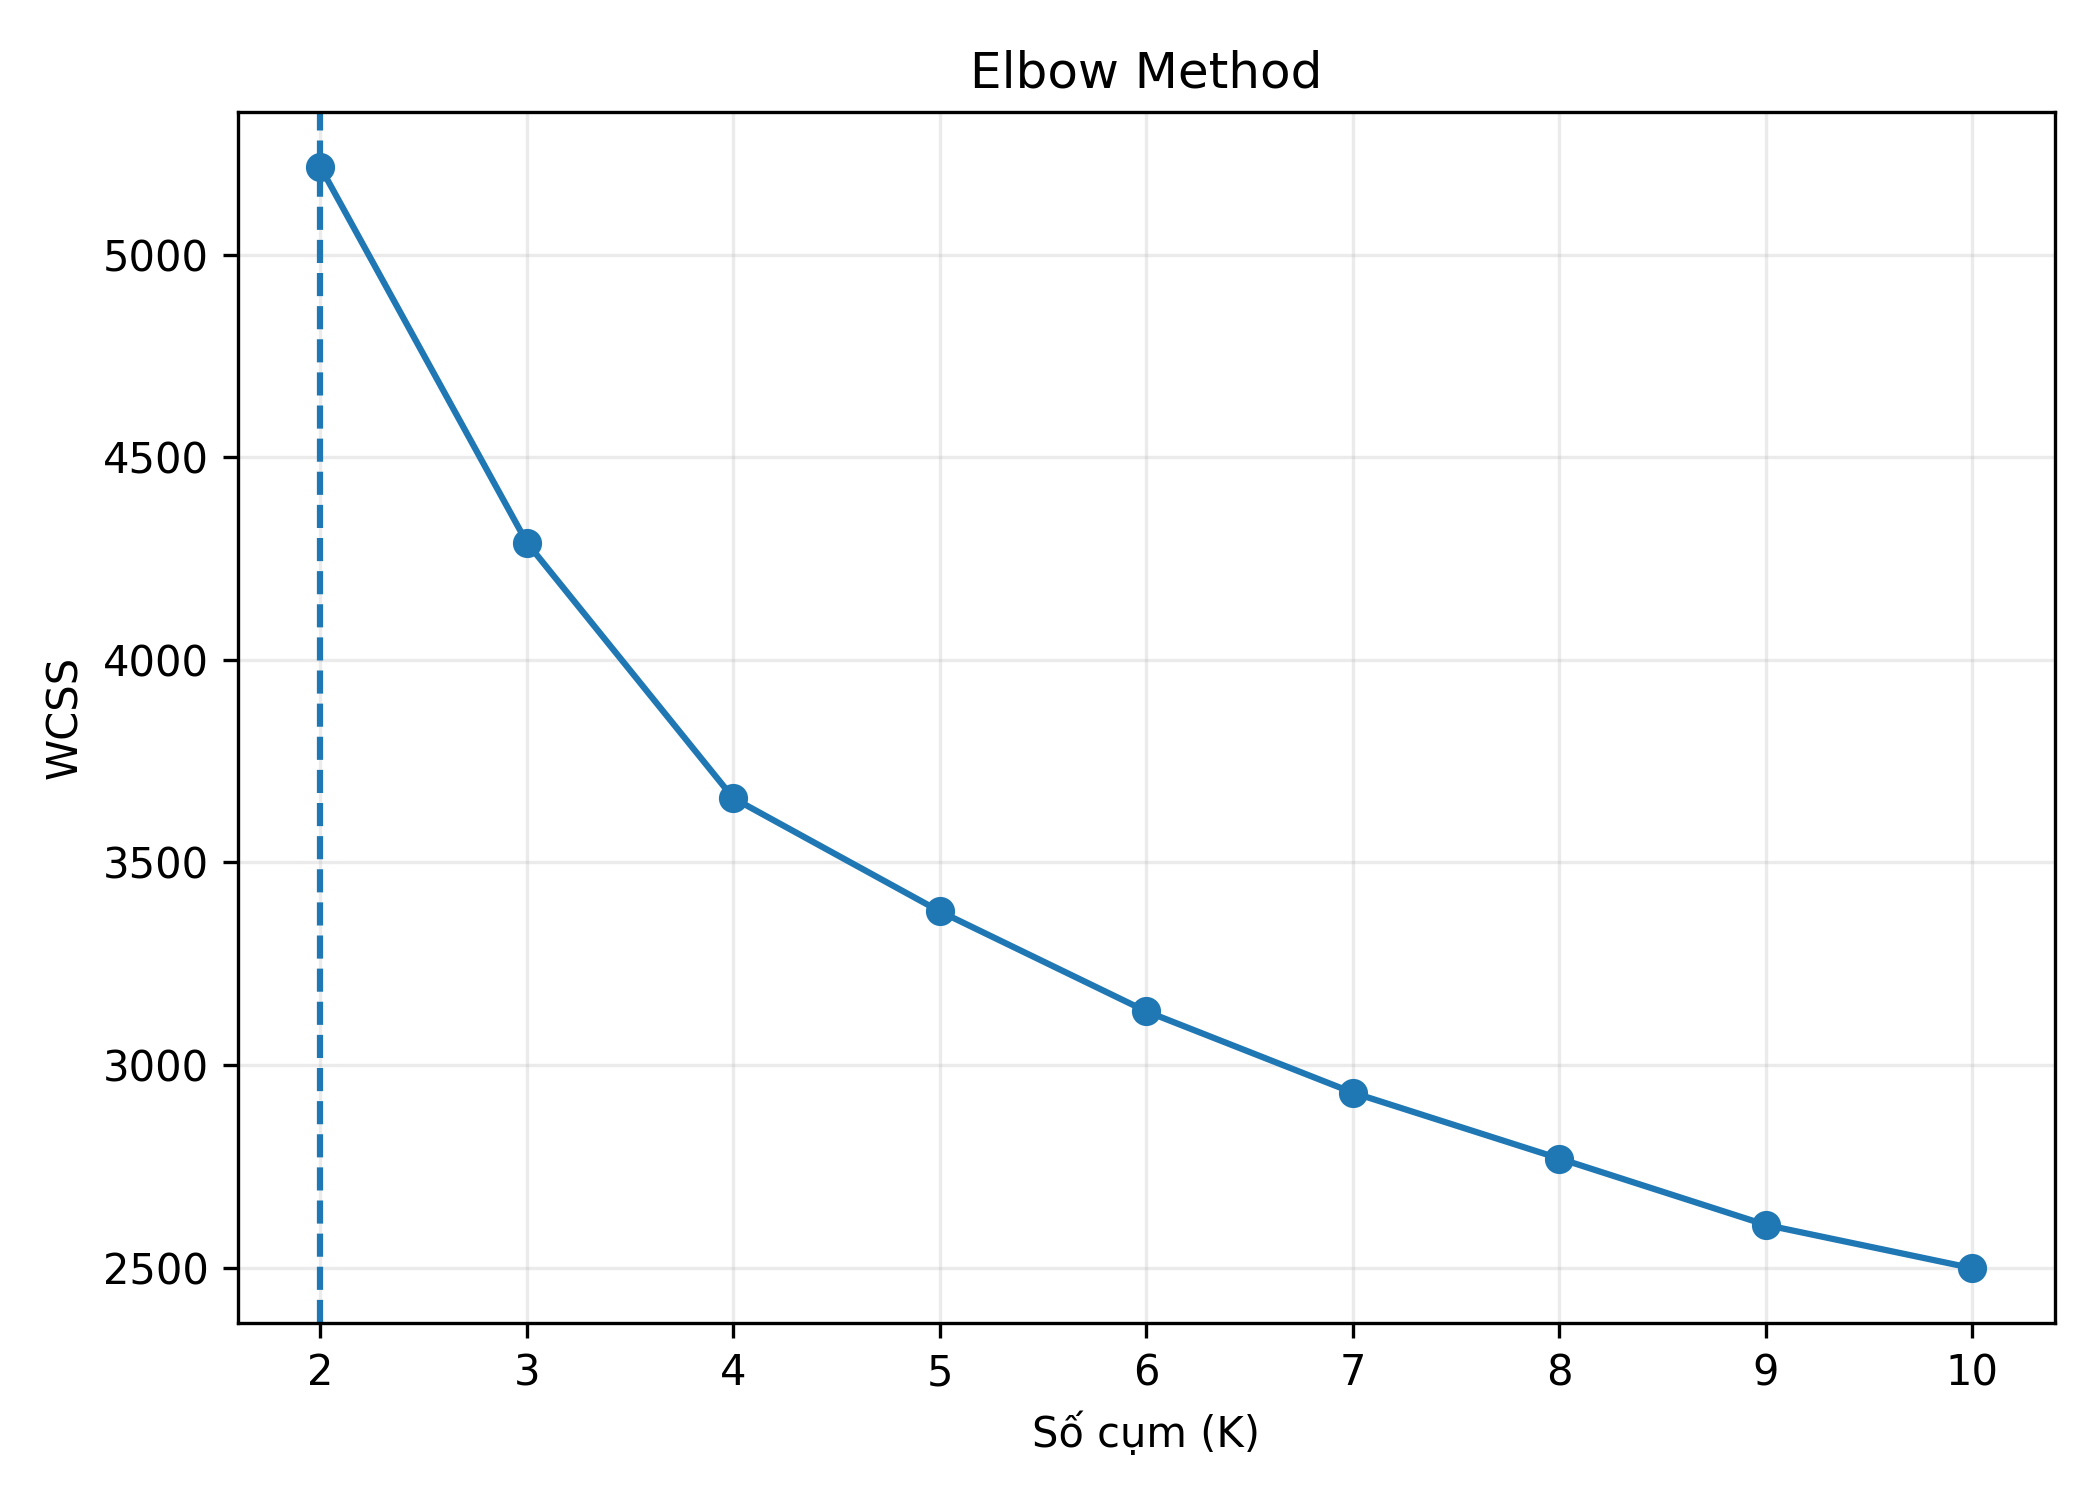
\includegraphics[width=0.7\textwidth]{images/anh_chuong4/kmeans_after_elbow.png}
	\caption{\centering Elbow Method của mô hình K-Means sau xử lý ngoại lai}
	\label{fig:kmeans_after_elbow}
\end{figure}

\begin{figure}[H]
	\centering
	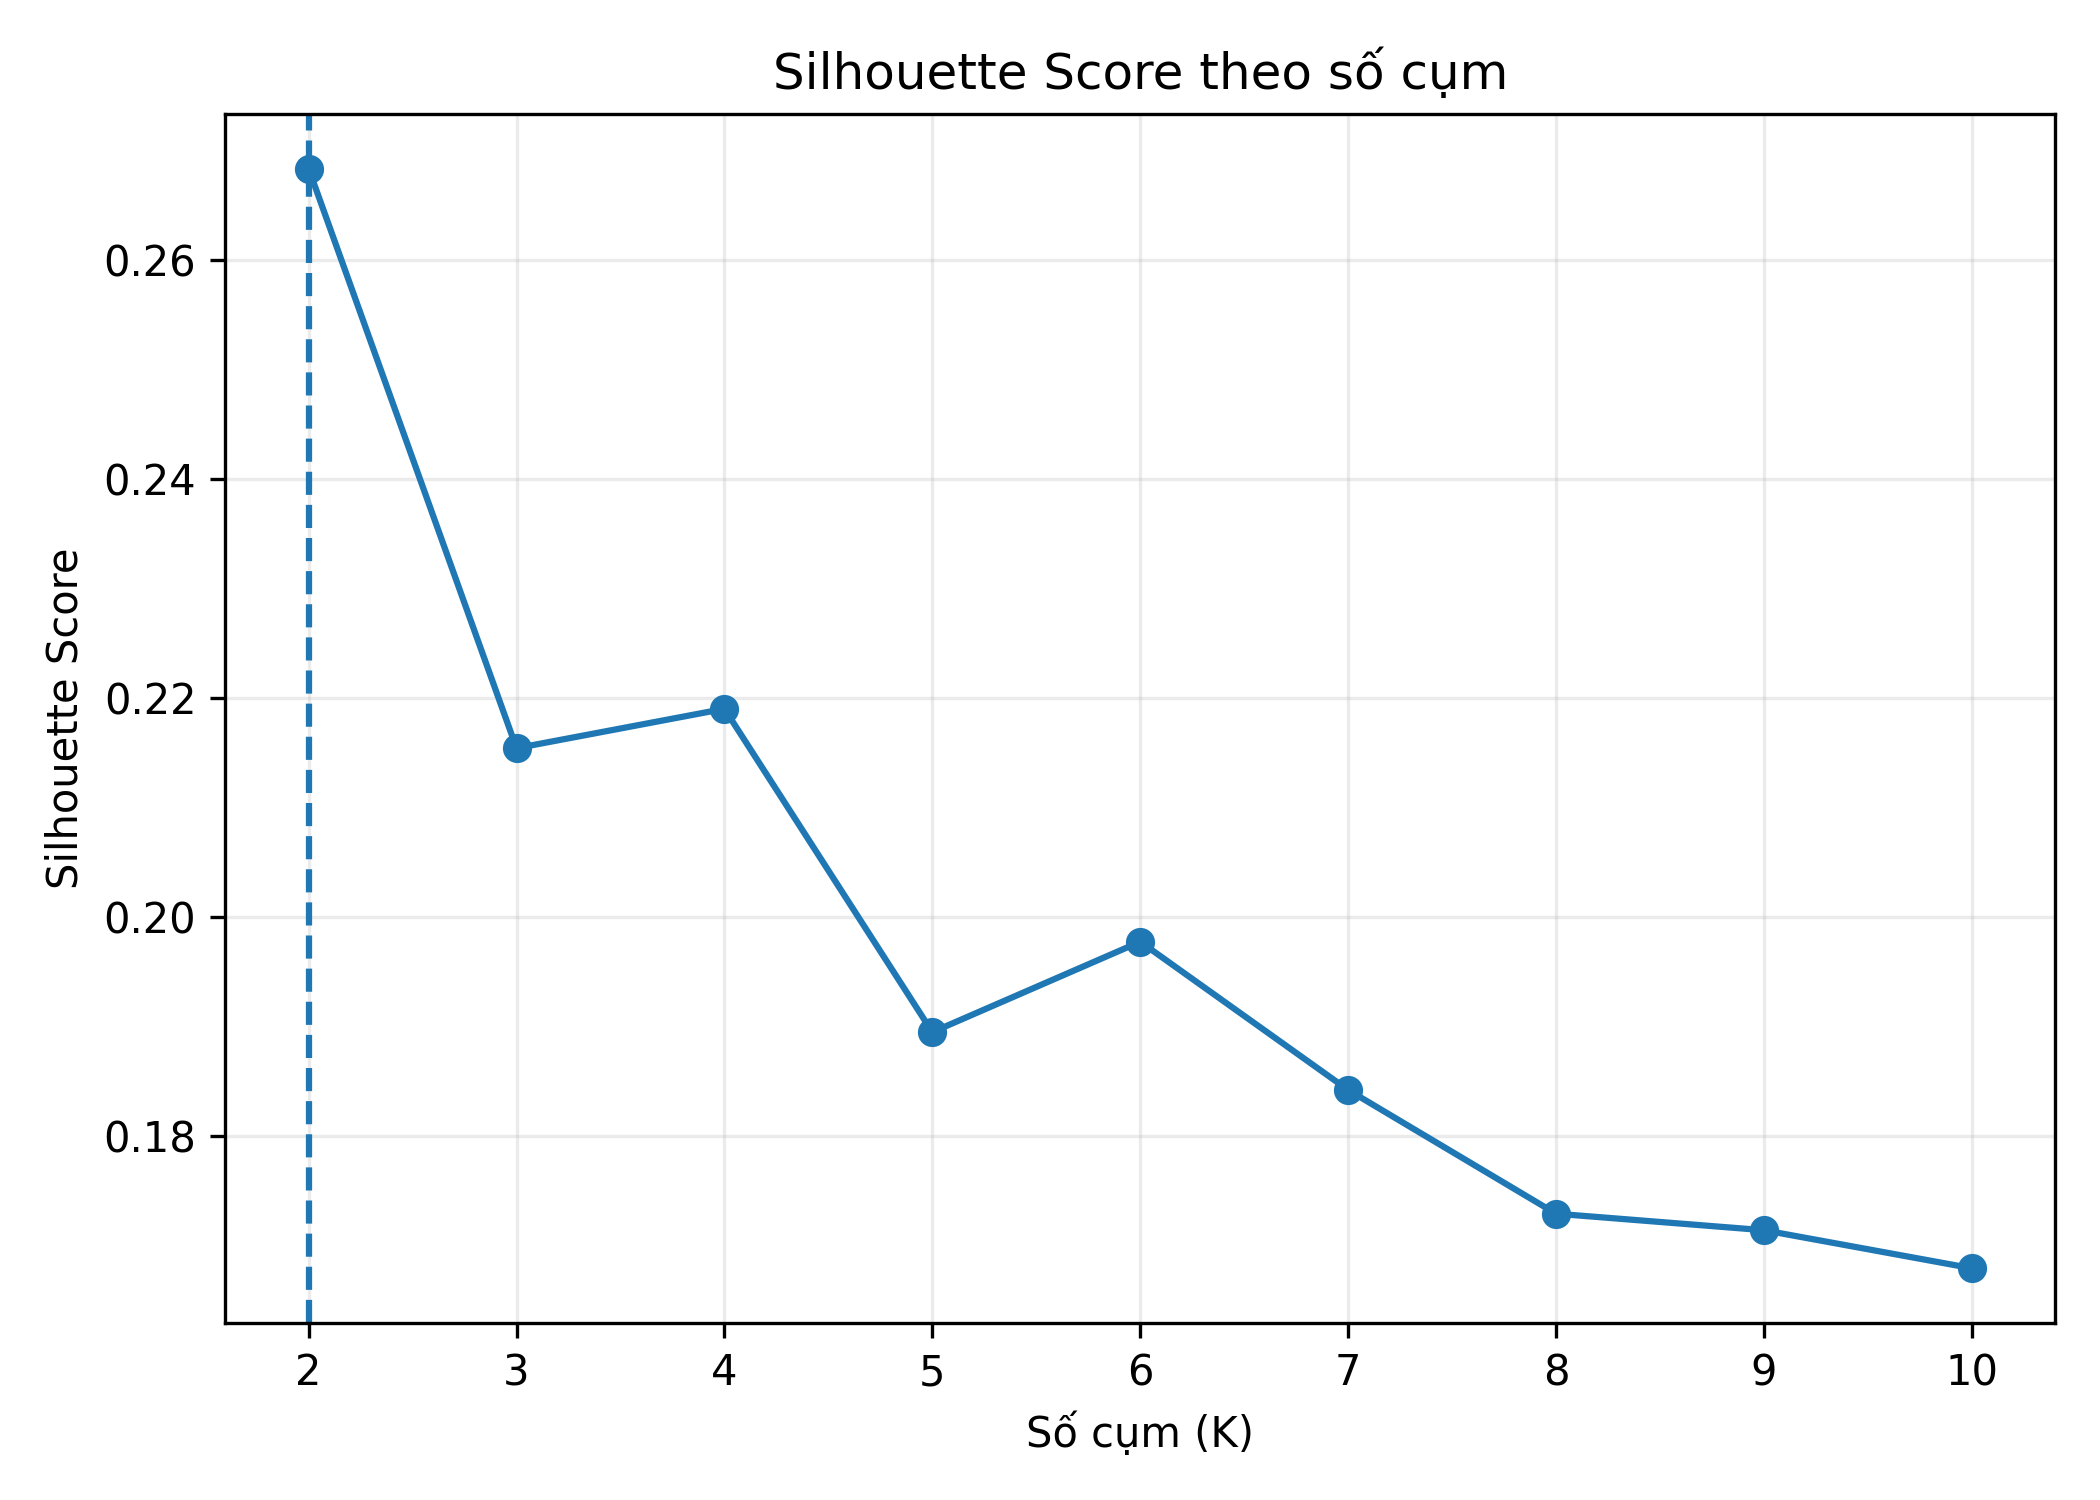
\includegraphics[width=0.7\textwidth]{images/anh_chuong4/kmeans_after_silhouette.png}
	\caption{\centering Silhouette Score của mô hình K-Means sau xử lý ngoại lai}
	\label{fig:kmeans_after_silhouette}
\end{figure}

Quan sát Hình \ref{fig:kmeans_after_elbow} và Hình \ref{fig:kmeans_after_silhouette} cho thấy WCSS giảm dần khi số cụm tăng, trong khi Silhouette Score đạt giá trị cao nhất tại \(K = 2\). Do đó, số cụm \(K = 2\) được lựa chọn để phân nhóm khách hàng sau xử lý ngoại lai.

\begin{figure}[H]
	\centering
	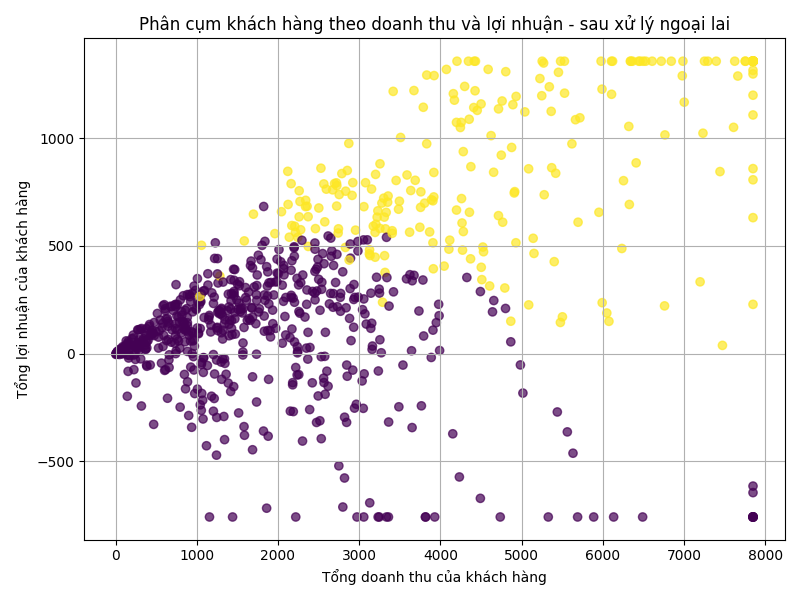
\includegraphics[width=0.8\textwidth]{images/anh_chuong4/kmeans_after_cluster.png}
	\caption{\centering Phân cụm khách hàng sau xử lý ngoại lai}
	\label{fig:kmeans_after_cluster}
\end{figure}

Quan sát Hình \ref{fig:kmeans_after_cluster} cho thấy các nhóm khách hàng được phân tách rõ ràng hơn so với trước xử lý ngoại lai. Một cụm tập trung nhiều khách hàng có doanh thu và lợi nhuận thấp hoặc trung bình, trong khi cụm còn lại đại diện cho nhóm khách hàng có giá trị cao hơn.

\begin{figure}[H]
	\centering
	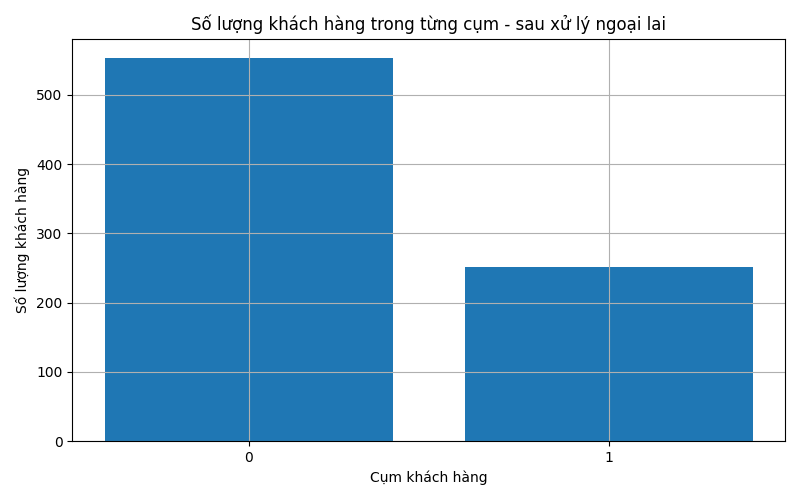
\includegraphics[width=0.65\textwidth]{images/anh_chuong4/kmeans_after_cluster_count.png}
	\caption{\centering Số lượng khách hàng trong từng cụm sau xử lý ngoại lai}
	\label{fig:kmeans_after_cluster_count}
\end{figure}

Biểu đồ số lượng khách hàng cho thấy hai cụm vẫn có sự chênh lệch về quy mô. Cụm 0 chiếm số lượng khách hàng lớn hơn, trong khi cụm 1 có ít khách hàng hơn nhưng thường đại diện cho nhóm có giá trị giao dịch cao hơn.

\begin{figure}[H]
	\centering
	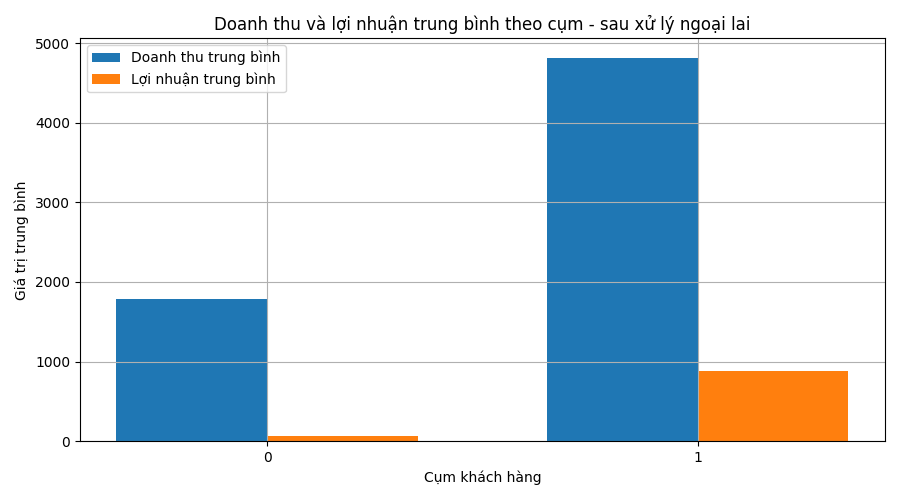
\includegraphics[width=0.75\textwidth]{images/anh_chuong4/kmeans_after_cluster_mean.png}
	\caption{\centering Doanh thu, lợi nhuận trung bình theo cụm sau xử lý ngoại lai}
	\label{fig:kmeans_after_cluster_mean}
\end{figure}

Quan sát Hình \ref{fig:kmeans_after_cluster_mean} cho thấy cụm 1 có doanh thu và lợi nhuận trung bình cao hơn rõ rệt so với cụm 0. Điều này cho thấy mô hình K-Means sau xử lý ngoại lai đã phản ánh tốt hơn sự khác biệt về giá trị giữa các nhóm khách hàng.

Nhìn chung, sau khi xử lý ngoại lai, kết quả phân cụm trở nên ổn định và dễ diễn giải hơn. Các cụm khách hàng không còn bị ảnh hưởng quá mạnh bởi các điểm dữ liệu cực đoan, từ đó hỗ trợ tốt hơn cho việc phân tích hành vi và giá trị khách hàng.

\refstepcounter{subsection}

\subsection*{\thesubsection\quad So sánh trước và sau xử lý ngoại lai}

Sau khi xử lý ngoại lai, kết quả phân cụm của mô hình K-Means trở nên ổn định và rõ ràng hơn. Các tâm cụm ít bị ảnh hưởng bởi các khách hàng có doanh thu hoặc lợi nhuận bất thường, giúp các cụm phản ánh chính xác hơn đặc điểm chung của từng nhóm khách hàng.

Ngoài ra, mức độ tách biệt giữa các cụm cũng được cải thiện sau khi dữ liệu được làm sạch. Điều này cho thấy việc xử lý ngoại lai giúp mô hình phân nhóm khách hàng hiệu quả hơn và nâng cao khả năng diễn giải kết quả.

Đối với K-Means, xử lý ngoại lai là bước quan trọng vì mô hình hoạt động dựa trên khoảng cách Euclid. Chỉ một số điểm dữ liệu cực đoan cũng có thể làm thay đổi vị trí tâm cụm và ảnh hưởng đến toàn bộ kết quả phân cụm. Vì vậy, việc kiểm soát ngoại lai giúp tăng độ tin cậy và tính ổn định của mô hình.

\refstepcounter{subsection}
\subsection*{\thesubsection\quad Nhận xét mô hình}

Kết quả phân cụm cho thấy khách hàng trong bộ dữ liệu có hành vi mua hàng và mức độ đóng góp lợi nhuận khác nhau. Một số nhóm khách hàng tạo ra doanh thu và lợi nhuận cao, trong khi một số nhóm khác có doanh thu tương đối lớn nhưng lợi nhuận thấp do ảnh hưởng của chiết khấu hoặc đặc điểm sản phẩm.

Điều này cho thấy doanh nghiệp không nên chỉ đánh giá khách hàng dựa trên doanh thu mà cần kết hợp thêm yếu tố lợi nhuận để xác định giá trị thực sự của từng nhóm khách hàng.

Kết quả của mô hình K-Means có ý nghĩa thực tiễn trong việc hỗ trợ phân khúc khách hàng và xây dựng chiến lược kinh doanh phù hợp. Doanh nghiệp có thể tập trung giữ chân nhóm khách hàng giá trị cao, đồng thời tối ưu chính sách chiết khấu và hoạt động bán hàng đối với các nhóm khách hàng có lợi nhuận thấp hơn.


	
	\chapter{Đánh giá và so sánh mô hình}
	\section{So sánh hiệu quả giữa các mô hình}

 Việc so sánh được thực hiện trên tập kiểm tra vì đây là phần dữ liệu chưa được sử dụng trong quá trình huấn luyện, do đó phản ánh tốt hơn khả năng tổng quát hóa của mô hình.

K-Means là mô hình học không giám sát phục vụ phân cụm khách hàng, mô hình này không được so sánh trực tiếp với các mô hình dự báo thông qua MAE, RMSE hay \(R^2\). Thay vào đó, K-Means được đánh giá thông qua Elbow Method, Silhouette Score và khả năng diễn giải các cụm khách hàng.

\begin{table}[H]
	\centering
	\caption{Tổng hợp kết quả các mô hình dự báo sau xử lý ngoại lai trên tập kiểm tra}
	\label{tab:model_result_after_outlier}
	\begin{tabular}{|l|r|r|r|r|}
		\hline
		\textbf{Mô hình} & \textbf{MAE} & \textbf{MSE} & \textbf{RMSE} & \textbf{\(R^2\)} \\ \hline
		Hồi quy tuyến tính đa biến & 18.4952 & 548.4677 & 23.4194 & 0.3617 \\ \hline
		Random Forest Regressor & 15.4900 & 438.9221 & 20.9505 & 0.4892 \\ \hline
		Gradient Boosting Regressor & 15.7957 & 426.5068 & 20.6520 & 0.5036 \\ \hline
		XGBoost Regressor & 15.5767 & 420.2505 & 20.5000 & 0.5109 \\ \hline
	\end{tabular}
\end{table}

Từ Bảng \ref{tab:model_result_after_outlier}, có thể thấy XGBoost Regressor đạt kết quả tốt nhất với \(R^2 = 0.5109\) và RMSE = 20.5000. Gradient Boosting cũng cho kết quả khá tốt với \(R^2 = 0.5036\). Random Forest có MAE thấp nhưng \(R^2\) thấp hơn XGBoost và Gradient Boosting. Trong khi đó, hồi quy tuyến tính đa biến có hiệu quả thấp nhất do khó mô hình hóa các quan hệ phi tuyến trong dữ liệu bán lẻ.

Nhìn chung, các mô hình học máy phi tuyến, đặc biệt là nhóm ensemble và boosting, phù hợp hơn với bài toán dự báo lợi nhuận so với mô hình tuyến tính. Điều này xuất phát từ đặc điểm dữ liệu bán lẻ, trong đó lợi nhuận chịu ảnh hưởng đồng thời bởi nhiều yếu tố như doanh thu, chiết khấu, số lượng bán, danh mục sản phẩm và khu vực.

\section{Lựa chọn mô hình phù hợp}

Dựa trên kết quả so sánh, XGBoost được lựa chọn là mô hình phù hợp nhất cho bài toán dự báo lợi nhuận trong phạm vi đề tài. Mô hình này đạt hệ số \(R^2\) cao nhất và RMSE thấp nhất trên tập kiểm tra, cho thấy khả năng dự báo tốt hơn các mô hình còn lại.

XGBoost phù hợp với dữ liệu bán lẻ vì có khả năng học các quan hệ phi tuyến và tương tác phức tạp giữa nhiều biến đầu vào. Bên cạnh đó, mô hình có cơ chế điều chuẩn giúp kiểm soát độ phức tạp và hạn chế hiện tượng quá khớp tốt hơn so với một số mô hình boosting thông thường.

Tuy nhiên, XGBoost có nhược điểm là khó diễn giải hơn hồi quy tuyến tính và cần quá trình xử lý dữ liệu, mã hóa biến định tính cũng như điều chỉnh tham số phù hợp. Vì vậy, trong đề tài này, hồi quy tuyến tính vẫn có ý nghĩa như mô hình nền để tham chiếu, còn XGBoost được xem là mô hình dự báo chính.

Đối với K-Means, mô hình không dùng để dự báo lợi nhuận mà phục vụ phân cụm khách hàng theo doanh thu và lợi nhuận. Kết quả phân cụm giúp bổ sung góc nhìn về hành vi và giá trị khách hàng, hỗ trợ doanh nghiệp nhận diện nhóm khách hàng tiềm năng và nhóm khách hàng cần tối ưu chính sách bán hàng.

\section{Ý nghĩa thực tiễn của kết quả mô hình}

Kết quả xây dựng mô hình không chỉ giúp so sánh hiệu quả dự báo mà còn hỗ trợ rút ra một số nhận xét có ý nghĩa thực tiễn đối với hoạt động kinh doanh bán lẻ. Các mô hình cho thấy lợi nhuận chịu ảnh hưởng bởi nhiều yếu tố như Discount, Sales, Quantity, Category, Sub-Category và đặc điểm khách hàng.

\begin{table}[H]
	\centering
	\caption{Ý nghĩa thực tiễn rút ra từ kết quả mô hình}
	\label{tab:practical_meaning_model}
	\renewcommand{\arraystretch}{1.3}
	\begin{tabular}{|p{3.2cm}|p{5.3cm}|p{5.3cm}|}
		\hline
		\textbf{Yếu tố} & \textbf{Kết quả rút ra} & \textbf{Ý nghĩa thực tiễn} \\ \hline
		
		Discount & Có ảnh hưởng lớn đến lợi nhuận, đặc biệt khi mức chiết khấu cao dễ đi kèm lợi nhuận thấp hoặc giao dịch lỗ. 
		& Doanh nghiệp cần kiểm soát chính sách chiết khấu hợp lý, tránh tăng doanh thu nhưng làm giảm lợi nhuận. \\ \hline
		
		Sales và Quantity & Có vai trò quan trọng trong dự báo lợi nhuận, nhưng doanh thu cao chưa chắc luôn đồng nghĩa với lợi nhuận cao. 
		& Cần đánh giá hiệu quả kinh doanh dựa trên cả doanh thu và lợi nhuận, không chỉ tập trung vào doanh số bán hàng. \\ \hline
		
		Category và Sub-Category & Một số nhóm sản phẩm có khả năng đóng góp lợi nhuận tốt hơn các nhóm khác. 
		& Doanh nghiệp có thể điều chỉnh chiến lược sản phẩm, giá bán và khuyến mãi theo từng nhóm hàng. \\ \hline
		
		K-Means Clustering & Giúp phân nhóm khách hàng dựa trên doanh thu và lợi nhuận. 
		& Hỗ trợ nhận diện nhóm khách hàng giá trị cao, nhóm khách hàng lợi nhuận thấp và xây dựng chính sách chăm sóc phù hợp. \\ \hline
		
		Dashboard và mô hình học máy & Dashboard giúp quan sát xu hướng, còn mô hình giúp lượng hóa mối quan hệ giữa các yếu tố và lợi nhuận. 
		& Kết hợp trực quan hóa và mô hình giúp nâng cao cơ sở ra quyết định dựa trên dữ liệu. \\ \hline
	\end{tabular}
\end{table}

Dashboard hỗ trợ quan sát xu hướng, trong khi mô hình học máy giúp đánh giá sâu hơn mối quan hệ giữa các yếu tố và lợi nhuận. Sự kết hợp này giúp kết quả phân tích có cơ sở hơn và hỗ trợ tốt hơn cho quá trình ra quyết định trong hoạt động kinh doanh bán lẻ.
	
	\chapter{Kết luận và hướng phát triển}
	\section{Kết luận chung}

Đồ án đã thực hiện quá trình phân tích doanh số và xu hướng tiêu dùng khách hàng trong lĩnh vực bán lẻ dựa trên bộ dữ liệu Superstore Sales. Thông qua các bước tiền xử lý dữ liệu, phân tích khám phá, trực quan hóa bằng Power BI và xây dựng các mô hình học máy, đề tài đã làm rõ được một số đặc điểm quan trọng trong hoạt động kinh doanh bán lẻ.

Kết quả phân tích cho thấy doanh thu, lợi nhuận và hành vi tiêu dùng của khách hàng có sự khác biệt theo thời gian, khu vực, danh mục sản phẩm và phân khúc khách hàng. Một số nhóm sản phẩm và khu vực có khả năng đóng góp lợi nhuận tốt, trong khi một số nhóm khác có doanh thu cao nhưng hiệu quả lợi nhuận chưa tương xứng. Đặc biệt, yếu tố chiết khấu có ảnh hưởng đáng kể đến lợi nhuận, cho thấy doanh nghiệp cần kiểm soát chính sách chiết khấu một cách hợp lý.

Bên cạnh đó, kết quả xây dựng mô hình cho thấy các mô hình học máy phi tuyến như Random Forest, Gradient Boosting và XGBoost cho hiệu quả dự báo tốt hơn so với hồi quy tuyến tính đa biến. Trong đó, XGBoost là mô hình đạt kết quả tốt nhất trên tập kiểm tra. Ngoài ra, mô hình K-Means Clustering cũng hỗ trợ phân nhóm khách hàng theo doanh thu và lợi nhuận, góp phần bổ sung góc nhìn về hành vi và giá trị khách hàng.

Nhìn chung, đề tài đã đạt được mục tiêu đề ra là khai thác dữ liệu bán hàng để phân tích tình hình kinh doanh, nhận diện xu hướng tiêu dùng và ứng dụng các mô hình phân tích dữ liệu nhằm hỗ trợ đánh giá, dự báo và ra quyết định dựa trên dữ liệu.

\section{Những kết quả đạt được}

Trong quá trình thực hiện, đồ án đã đạt được một số kết quả chính như sau:

\begin{itemize}
	\item Hệ thống hóa được cơ sở lý thuyết liên quan đến phân tích dữ liệu trong kinh doanh, trực quan hóa dữ liệu, tiền xử lý dữ liệu và các mô hình học máy sử dụng trong đề tài.
	
	\item Thực hiện quá trình tiền xử lý dữ liệu, kiểm tra dữ liệu thiếu, dữ liệu trùng lặp, chuẩn hóa kiểu dữ liệu và xử lý ngoại lai, giúp dữ liệu phù hợp hơn cho phân tích và xây dựng mô hình.
	
	\item Phân tích khám phá dữ liệu nhằm làm rõ đặc điểm doanh thu, lợi nhuận, số lượng bán, chiết khấu, khu vực bán hàng, danh mục sản phẩm và phân khúc khách hàng.
	
	\item Xây dựng dashboard trên Power BI để trực quan hóa các chỉ tiêu quan trọng, giúp quan sát tình hình kinh doanh một cách rõ ràng và trực quan hơn.
	
	\item Xây dựng và đánh giá các mô hình dự báo lợi nhuận gồm hồi quy tuyến tính đa biến, Random Forest, Gradient Boosting và XGBoost. Kết quả cho thấy XGBoost là mô hình phù hợp nhất trong phạm vi đề tài.
	
	\item Ứng dụng mô hình K-Means Clustering để phân cụm khách hàng, từ đó hỗ trợ nhận diện các nhóm khách hàng có đặc điểm khác nhau về doanh thu và lợi nhuận.
	
	\item Rút ra được một số nhận xét có ý nghĩa thực tiễn, đặc biệt là vai trò của chiết khấu, doanh thu, số lượng bán và nhóm sản phẩm đối với lợi nhuận trong dữ liệu bán lẻ.
\end{itemize}

\section{Hạn chế tồn đọng của đề tài}

Mặc dù đã đạt được một số kết quả nhất định, đề tài vẫn còn tồn tại một số hạn chế. Trước hết, bộ dữ liệu sử dụng là dữ liệu có sẵn nên chưa phản ánh đầy đủ toàn bộ các yếu tố thực tế có thể ảnh hưởng đến hoạt động kinh doanh, chẳng hạn như chi phí vận hành, chính sách marketing, hành vi khách hàng chi tiết hoặc yếu tố cạnh tranh thị trường.

Thứ hai, các mô hình dự báo trong đề tài mới được xây dựng ở mức cơ bản, chủ yếu nhằm so sánh hiệu quả giữa các thuật toán. Việc tối ưu tham số mô hình chưa được thực hiện chuyên sâu, do đó kết quả dự báo vẫn có thể được cải thiện thêm nếu áp dụng các kỹ thuật tối ưu phù hợp.

Thứ ba, mô hình K-Means mới chỉ phân cụm khách hàng dựa trên một số đặc điểm chính như doanh thu và lợi nhuận. Trong thực tế, việc phân nhóm khách hàng có thể cần kết hợp thêm nhiều yếu tố khác như tần suất mua hàng, giá trị trung bình mỗi đơn hàng, thời gian mua gần nhất và hành vi mua theo từng nhóm sản phẩm.

Ngoài ra, dashboard trong đề tài chủ yếu phục vụ mục tiêu trực quan hóa và phân tích mô tả. Việc tích hợp trực tiếp kết quả dự báo từ mô hình vào dashboard chưa được triển khai, nên khả năng hỗ trợ ra quyết định theo thời gian thực vẫn còn hạn chế.

\section{Hướng phát triển trong tương lai}

Trong tương lai, đề tài có thể được phát triển theo một số hướng sau:

\begin{itemize}
	\item \textbf{Mở rộng dữ liệu nghiên cứu:} 
	Có thể bổ sung thêm các dữ liệu liên quan đến chi phí vận hành, chương trình khuyến mãi, hành vi khách hàng và dữ liệu thị trường. Việc mở rộng dữ liệu giúp kết quả phân tích phản ánh sát hơn bối cảnh kinh doanh thực tế.
	
	\item \textbf{Tối ưu mô hình dự báo:} 
	Các mô hình học máy có thể được cải thiện bằng cách tối ưu tham số thông qua Grid Search, Random Search hoặc Cross Validation. Điều này giúp nâng cao độ chính xác dự báo và khả năng tổng quát hóa trên dữ liệu mới.
	
	\item \textbf{Phát triển phân cụm khách hàng chuyên sâu hơn:} 
	Đối với bài toán phân cụm, có thể kết hợp thêm phương pháp RFM gồm Recency, Frequency và Monetary Value. Cách tiếp cận này giúp phân nhóm khách hàng chi tiết hơn, hỗ trợ tốt hơn cho hoạt động chăm sóc khách hàng và marketing.
	
	\item \textbf{Nâng cấp dashboard trực quan:} 
	Dashboard Power BI có thể được phát triển thêm theo hướng tương tác sâu hơn, cho phép người dùng theo dõi dữ liệu theo thời gian, khu vực, nhóm sản phẩm và phân khúc khách hàng. Ngoài ra, có thể tích hợp kết quả dự báo từ mô hình vào dashboard.
	
	\item \textbf{Xây dựng hệ thống phân tích dữ liệu tự động:} 
	Một hướng phát triển quan trọng là xây dựng thành website, phần mềm hoặc hệ thống hỗ trợ phân tích dữ liệu bán hàng tự động. Khi đó, người dùng chỉ cần tải bộ dữ liệu lên hệ thống, phần mềm sẽ tự động kiểm tra dữ liệu, làm sạch dữ liệu, trực quan hóa, xây dựng mô hình dự báo và xuất báo cáo phân tích cơ bản.
\end{itemize}

Tóm lại, đề tài là bước đầu trong việc vận dụng phân tích dữ liệu, trực quan hóa và học máy vào bài toán kinh doanh bán lẻ. Các kết quả đạt được có thể làm nền tảng để tiếp tục phát triển các hệ thống phân tích, dự báo và hỗ trợ ra quyết định trong thực tiễn.	
	
	
	
	%\addcontentsline{toc}{chapter}{Kết luận}
	%\setcounter{section}{0}
	%\renewcommand*{\thesection}{\the\value{section}}
	
		
	%================ PHỤ LỤC ================
	\clearpage
	\phantomsection
	\chapter*{Phụ lục}
	\addcontentsline{toc}{chapter}{Phụ lục}
	
	Trong quá trình thực hiện đồ án, bộ dữ liệu và một số tài liệu liên quan được em lưu trữ tại các đường dẫn sau:
	
	\begin{itemize}
		\item \textbf{Link bộ dữ liệu Superstore Sales:} \\
		\url{https://public.tableau.com/app/learn/sample-data}
		
		\item \textbf{Link GitHub lưu trữ dữ liệu đồ án:} \\
		\url{https://github.com/nguyenhuunhatanh/DoAn1-Superstore_Sales}
	\end{itemize}
	
	
	%================ TÀI LIỆU THAM KHẢO ================
	\clearpage
	\phantomsection
	\addcontentsline{toc}{chapter}{\bfseries Tài liệu tham khảo}
	
	{\sloppy
		\begin{thebibliography}{99}
			
			\bibitem{islr}
			James, G., Witten, D., Hastie, T., Tibshirani, R.
			\textit{An Introduction to Statistical Learning: with Applications in R}.
			2nd Edition, Springer, 2021.
			
			\bibitem{esl}
			Hastie, T., Tibshirani, R., Friedman, J.
			\textit{The Elements of Statistical Learning: Data Mining, Inference, and Prediction}.
			2nd Edition, Springer, 2009.
			
			\bibitem{geron}
			Géron, A.
			\textit{Hands-On Machine Learning with Scikit-Learn, Keras, and TensorFlow}.
			3rd Edition, O'Reilly Media, 2022.
			
			\bibitem{few}
			Few, S.
			\textit{Show Me the Numbers: Designing Tables and Graphs to Enlighten}.
			2nd Edition, Analytics Press, 2012.
			
			\bibitem{powerbi}
			Microsoft.
			\textit{What is business intelligence?}
			Microsoft Learn, 2025.\\
			Available at: \url{https://learn.microsoft.com/en-us/power-bi/fundamentals/}
			
			\bibitem{sklearn_linear}
			Scikit-learn Developers.
			\textit{Linear Models}.
			Scikit-learn Documentation, 2025.\\
			Available at: \url{https://scikit-learn.org/stable/modules/linear_model.html}
			
			\bibitem{sklearn_rf}
			Scikit-learn Developers.
			\textit{RandomForestRegressor}.
			Scikit-learn Documentation, 2025.\\
			Available at: \url{https://scikit-learn.org/stable/modules/generated/sklearn.ensemble.RandomForestRegressor.html}
			
			\bibitem{sklearn_gbr}
			Scikit-learn Developers.
			\textit{GradientBoostingRegressor}.
			Scikit-learn Documentation, 2025.\\
			Available at: \url{https://scikit-learn.org/stable/modules/generated/sklearn.ensemble.GradientBoostingRegressor.html}
			
			\bibitem{chen2016xgboost}
			Chen, T., Guestrin, C.
			\textit{XGBoost: A Scalable Tree Boosting System}.
			Proceedings of the 22nd ACM SIGKDD International Conference on Knowledge Discovery and Data Mining, 2016, pp.~785--794.
			
			\bibitem{sklearn_kmeans}
			Scikit-learn Developers.
			\textit{KMeans}.
			Scikit-learn Documentation, 2025.\\
			Available at: \url{https://scikit-learn.org/stable/modules/generated/sklearn.cluster.KMeans.html}
			
			\bibitem{sklearn_silhouette}
			Scikit-learn Developers.
			\textit{silhouette\_score}.
			Scikit-learn Documentation, 2025.\\
			Available at: \url{https://scikit-learn.org/stable/modules/generated/sklearn.metrics.silhouette_score.html}
			
			\bibitem{sklearn_userguide}
			Scikit-learn Developers.
			\textit{Scikit-learn User Guide}.
			Scikit-learn Documentation, 2025.\\
			Available at: \url{https://scikit-learn.org/stable/user_guide.html}
			
		\end{thebibliography}
	}
	
\end{document}
